\documentclass[a4paper,final,12pt,twoside]{class_diss}

% +--------------------------------------------------------------------+
% | The following command sets the bibliography style to American
% | Institute of Physics (AIP).  Other styles are available in the
% | styles directory.  To use a different style, replace "aip" with
% | the filename of the style you want to use.
% +--------------------------------------------------------------------+

%\bibliographystyle{styles/plain}

\usepackage[utf8]{inputenc}
\usepackage[T1]{fontenc}
\usepackage[spanish]{babel}
\selectlanguage{spanish}
\usepackage{eurosym}

% +--------------------------------------------------------------------+
% | Now, we add in all external packages that we will use throughout   |
% | the document.  You can add other packages as needed.
% +--------------------------------------------------------------------+

%\usepackage{     caption2} % Customize captions a bit more
\usepackage{      amsmath} % American Mathematics Society standards
%\usepackage{      wrapfig} % Wraps text around a figure or table
\usepackage{     graphicx} % Extended graphics package.
\usepackage{subfig}

%\usepackage{     fancyhdr} % Efficiently handles headers and footers
%\usepackage{       braket} % Bra-Ket notation package
%\usepackage{     mathrsfs} % Specialized Math fonts (Hamiltonian, etc.)
%\usepackage{boxedminipage} % Boxed text can be produced
%\usepackage{     setspace} % Controls line spacing via \begin{space}

\usepackage{amsxtra}
\usepackage{amssymb}
\usepackage{amsthm}
\usepackage{latexsym}

\usepackage{enumerate}
\usepackage{float}

% +--------------------------------------------------------------------+
% | The color package allows one to select colors for hyperlinking     |
% | (see below).                                                       |
% +--------------------------------------------------------------------+

\usepackage[usenames]{color}

% +--------------------------------------------------------------------+
% | Colors defined for use with this template.                         |
% +--------------------------------------------------------------------+

\definecolor{  Pink}{rgb}{1.0, 0.5, 0.5}
\definecolor{Maroon}{rgb}{0.8, 0.0, 0.0}

% +--------------------------------------------------------------------+
% | In the commands below, we use the 'natbib' package, and specify    |
% | the 'sort&compress' option, which condenses                        |
% | citations from (1,2,3,5,9,10,11) to (1-3,5,9-11).  The 'bibpunct'  |
% | option selects various parameters for how the citation will be     |
% | displayed.  In this case, only the comma (separation between       |
% | citations) and the 's' (superscript) arguments are chosen.  The    |
% | other curly braces deal with how to 'wrap' the citation (using     |
% | parentheses, brackets, etc.) and are not needed for the chosen     |
% | style.                                                             |
% +--------------------------------------------------------------------+

\usepackage[sort&compress]{natbib}

\newcommand*{\nota}{\textcolor{red}}

%\bibpunct{}{}{,}{s}{}{}
%\usepackage{hypernat}

% +--------------------------------------------------------------------+
% | Lastly, the hyperref package allows one to hyperlink cross-        |
% | references and figures in a LaTeX document.                        |
% +--------------------------------------------------------------------+

\usepackage[pdftex, plainpages=false, pdfpagelabels]{hyperref}
\usepackage{url}
\usepackage{listings}
\usepackage{minted}
\hypersetup{
    linktocpage=true,
    colorlinks=true,
    bookmarks=true,
    citecolor=blue,
    urlcolor=red,
    linkcolor=Maroon,
    citebordercolor={1 0 0},
    urlbordercolor={1 0 0},
    linkbordercolor={.7 .8 .8},
    breaklinks=true,
    pdfpagelabels=true,
    }

\usepackage{color}

\definecolor{mygreen}{rgb}{0,0.6,0}
\definecolor{mygray}{rgb}{0.5,0.5,0.5}
\definecolor{mymauve}{rgb}{0.58,0,0.82}

\lstset{ %
literate=%
         {á}{{\'a}}1
         {í}{{\'i}}1
         {é}{{\'e}}1
         {ý}{{\'y}}1
         {ú}{{\'u}}1
         {ó}{{\'o}}1
         {ě}{{\v{e}}}1
         {š}{{\v{s}}}1
         {č}{{\v{c}}}1
         {ř}{{\v{r}}}1
         {ž}{{\v{z}}}1
         {ď}{{\v{d}}}1
         {ť}{{\v{t}}}1
         {ň}{{\v{n}}}1                
         {ů}{{\r{u}}}1
         {Á}{{\'A}}1
         {Í}{{\'I}}1
         {É}{{\'E}}1
         {Ý}{{\'Y}}1
         {Ú}{{\'U}}1
         {Ó}{{\'O}}1
         {Ě}{{\v{E}}}1
         {Š}{{\v{S}}}1
         {Č}{{\v{C}}}1
         {Ř}{{\v{R}}}1
         {Ž}{{\v{Z}}}1
         {Ď}{{\v{D}}}1
         {Ť}{{\v{T}}}1
         {Ň}{{\v{N}}}1                
         {Ů}{{\r{U}}}1,
  backgroundcolor=\color{white},   % choose the background color; you must add \usepackage{color} or \usepackage{xcolor}; should come as last argument
  basicstyle=\footnotesize,        % the size of the fonts that are used for the code
  breakatwhitespace=false,         % sets if automatic breaks should only happen at whitespace
  breaklines=true,                 % sets automatic line breaking
  captionpos=b,                    % sets the caption-position to bottom
  commentstyle=\color{mygreen},    % comment style
  deletekeywords={...},            % if you want to delete keywords from the given language
  escapeinside={\%*}{*)},          % if you want to add LaTeX within your code
  extendedchars=true,              % lets you use non-ASCII characters; for 8-bits encodings only, does not work with UTF-8
  frame=,	                   % adds a frame around the code
  keepspaces=true,                 % keeps spaces in text, useful for keeping indentation of code (possibly needs columns=flexible)
  keywordstyle=\color{blue},       % keyword style
  language=C++,                 % the language of the code
  morekeywords={*,...},            % if you want to add more keywords to the set
  numbers=left,                    % where to put the line-numbers; possible values are (none, left, right)
  numbersep=5pt,                   % how far the line-numbers are from the code
  numberstyle=\tiny\color{mygray}, % the style that is used for the line-numbers
  rulecolor=\color{black},         % if not set, the frame-color may be changed on line-breaks within not-black text (e.g. comments (green here))
  showspaces=false,                % show spaces everywhere adding particular underscores; it overrides 'showstringspaces'
  showstringspaces=false,          % underline spaces within strings only
  showtabs=false,                  % show tabs within strings adding particular underscores
  stepnumber=2,                    % the step between two line-numbers. If it's 1, each line will be numbered
  stringstyle=\color{mymauve},     % string literal style
  tabsize=2,	                   % sets default tabsize to 2 spaces
  title=\lstname                   % show the filename of files included with \lstinputlisting; also try caption instead of title
}

\renewcommand{\lstlistingname}{Código}% Listing -> Algorithm
\renewcommand{\lstlistlistingname}{Índice de códigos}% List of Listings -> List of Algorithms

\lstdefinestyle{lua}{
  backgroundcolor=\color{white},
  language=[5.1]Lua,
  basicstyle=\footnotesize,    
  breakatwhitespace=false,     
  breaklines=true,             
  captionpos=b,                
  commentstyle=\color{mygreen},
  deletekeywords={...},        
  escapeinside={\%*}{*)},      
  extendedchars=true,          
  frame=,	                   
  keepspaces=true,             
  keywordstyle=\color{blue},   
  morekeywords={*,...},        
  numbers=left,                
  numbersep=5pt,               
  stringstyle=\color{magenta},
  numberstyle=\tiny\color{mygray},
  rulecolor=\color{black},        
  showspaces=false,               
  showstringspaces=false,         
  showtabs=false,                 
  stepnumber=2,                   
  stringstyle=\color{mymauve},    
  tabsize=2,	                  
  title=\lstname                  
}

%\topmargin      = -0.56in
\textheight     =  8.20in
\textwidth      =  6.46in
\oddsidemargin  =  0.12in
\evensidemargin = -0.10in

\begin{document}

% +--------------------------------------------------------------------+
% | Title Page
% +--------------------------------------------------------------------+

\newpage

% +--------------------------------------------------------------------+
% | This page should not contain a page number.  We use the
% | \thispagestyle[empty] command below to suppress page numbers
% | and other style elements.
% +--------------------------------------------------------------------+

\thispagestyle{empty}

% +--------------------------------------------------------------------+
% | The Title page begins here.
% +--------------------------------------------------------------------+

\begin{center}

   \vspace{1cm}

% +--------------------------------------------------------------------+
% | On the line below, replace "ENTER YOUR TITLE" with the title of
% | your ETDR.  Use all CAPITAL LETTERS.
% +--------------------------------------------------------------------+

   {\Large Diseño y despliegue de un clúster de
bajo presupuesto para el desarrollo de
las prácticas de PSD
}\\

   \vspace{0.5cm}



   \vspace{0.5cm}



   {\large Daniel Quiñones Sánchez}\\
   {\large Miguel Romero Martínez}\\

   \vspace{0.5cm}



   Grado en Ingeniería de Computadores\\
   Facultad de Informática\\ 


   \vspace{0.65cm}
   \rule{2in}{0.5pt}\\
   \vspace{0.85cm}

  
\includegraphics[height=2.5in]{pics/escudo.png}
  

%+-- Escribe el nombre de tu asignatura de fin de master (Ingeniería de computadores,....)
   \vspace{0.5cm}
   Universidad Complutense de Madrid \\
   \vspace{0.5cm}





% +--------------------------------------------------------------------+
%  Fecha 
% +--------------------------------------------------------------------+

  Curso Académico 2017/2018\\
   \vspace{1cm}

\end{center}

{\raggedleft
Directores:\\
   \vspace{ 1cm}
Alberto Núñez Covarrubias\\
Luis Llana Díaz\\
}



% +--------------------------------------------------------------------+
% | Use the section below if you have co-major professors.
% +--------------------------------------------------------------------+

%\begin{flushleft}
%   \hspace{10cm}Approved by:\\
%   \vspace{ 1cm}
%   \hspace{10cm}Co-Major Professor\\
%   \hspace{10cm}Enter Your Co-Major Professor's Name\\
%   \vspace{.5cm}
%   \hspace{10cm}Co-Major Professor\\
%   \hspace{10cm}Enter Your Co-Major Professor's Name\\
%\end{flushleft}



   \pdfbookmark[0]{Portada}{PDFPortadaPage}

%///////////////////////////////////////////////////////
\newpage
$\ $
\thispagestyle{empty} % para que no se numere esta pagina
%///////////////////////////////////////////////////////

\newpage
\begin{center}
{\bf \Huge Agradecimientos}
\end{center}
\vspace{1cm}
\setlength{\baselineskip}{0.8cm}

\begin{figure}[H]
	\raggedleft
  	
\includegraphics[width=12mm]{pics/sonic_.png}
\end{figure}

\begin{flushright}
\textit{A mi compañero y amigo Rome, por aguantarme en todo momento y realizar la mayor parte del trabajo.}\\
Daniel\\
\vspace{0.5cm}


\begin{figure}[H]
	\raggedleft
  	
\includegraphics[width=12mm]{pics/knuckles.png}
\end{figure}

\textit{A mi compañero y amigo Daniel, por aguantarme en todo momento y realizar la mayor parte del trabajo.}\\
Miguel\\
\vspace{0.5cm}

\begin{figure}[H]
	\raggedleft
  	
\includegraphics[width=15mm]{pics/both.png}
\end{figure}

\textit{}\\
Daniel \&\& Miguel\\
\vspace{0.5cm}


\end{flushright}



\thispagestyle{empty}
\phantomsection

%///////////////////////////////////////////////////////
\newpage
$\ $
\thispagestyle{empty} % para que no se numere esta pagina
%///////////////////////////////////////////////////////

\newpage
\pagenumbering{roman}
\setcounter{page}{1}
\phantomsection
\addcontentsline{toc}{chapter}{}

\cleardoublepage
\tableofcontents
\cleardoublepage
\listoffigures

%---------------------------------------------------------------------
%
%                      abstract.tex
%
%---------------------------------------------------------------------
%
% Contiene el cap�tulo del resumen en ingl�s.
%
% Se crea como un cap�tulo sin numeraci�n.
%
%---------------------------------------------------------------------

\chapter{Abstract}
% Variable local para emacs, para  que encuentre el fichero maestro de
% compilaci�n y funcionen mejor algunas teclas r�pidas de AucTeX
%%%
%%% Local Variables:
%%% mode: latex
%%% TeX-master: "../Tesis.tex"
%%% End:

\addcontentsline{toc}{chapter}{Abstract}
\pdfbookmark[0]{Abstract}{PDFAbstractPage}
\vfill  
%///////////////////////////////////////////////////////
\newpage
$\ $
\thispagestyle{empty} % para que no se numere esta pagina
%///////////////////////////////////////////////////////
\newpage
\pagenumbering{arabic}
\setcounter{page}{1}
\newpage

\chapter{Introducción}

\label{ch:capitulo1.tex}

\begin{FraseCelebre}
	\begin{Frase}
		However difficult life may seem, there is always something you can do, and succeed at. It matters that you don’t just give up.
	\end{Frase}
	\begin{Fuente}
	Stephen William Hawking
	\end{Fuente}
\end{FraseCelebre}

\paragraph{}
El objetivo principal de este trabajo es el desarrollo de un clúster de cómputo de bajo presupuesto. Para ello hemos hecho uso de los denominados computadores de placa reducida, \textbf{Raspberry Pi}, como nodos de procesamiento sobre una distribución de linux \textit{Debian Jessie}. 

Nos planteamos los siguientes objetivos específicos: diseño del contenedor, distribución de cada uno de los elementos dentro de éste, estudio de las temperaturas y comportamiento del Hardware bajo situaciones de estrés, despliegue y desarrollo del software del sistema, estudio de rendimiento del mismo, generación de guías de instalación y aspectos específicos de configuración del sistema, desarrollo de un planificador de tareas para la distribución de trabajos entre los nodos y desarrollo de un  software para realizar el envío y recepción de trabajos al clúster.

A lo largo del documento se irán desarrollando cada uno de los puntos anteriores.

Este trabajo está destinado a complementar las prácticas de laboratorio que se realizan en la asignatura de \textit{Programación de Sistemas Distribuidos} (PSD) en la \textit{Facultad de Informática} de la \textbf{Universidad Complutense de Madrid}, al finalizar el proyecto, el cluster, permitirá a los alumnos la posibilidad de realizar algunas de las tareas de cómputo sobre él, servirá además como ejemplo de un sistema distribuido real, con el que poder afianzar los conocimientos de la asignatura.

\section{Motivación}
\label{makereference1.2}
\paragraph{}
En los últimos años se ha incrementado ese tipo de proyectos por parte de distintas universidades e iniciativas de particulares. Principalmente estos se han centrado en aumentar el número de dispositivos en cada proyecto, pero no existe un estudio de comportamiento real de uno de ellos, así como una guía que establezca los pasos a seguir, nuestro propósito ha sido el de reflejar todos los aspectos del desarrollo de uno de estos clusteres, centrándonos particularmente en la correcta disposición y distribución de los componentes para mejorar aspectos como la accesibilidad, la correcta refrigeración de los nodos y la mejora del rendimiento en ellos.


\section{Objetivos}
\label{makereference1.3}
\paragraph{}
Existen multitud de proyectos de este tipo, destacaremos los mas interesantes: 

\begin{itemize}

\item \href{http://web.eece.maine.edu/~vweaver/projects/pi-cluster}{VMW Research Group Raspberry Pi Cluster}, dispone de un clúster de 24 nodos realizado con raspberry Pi 2 con una interfaz de pantalla táctil y dos adaptadores de Ethernet que controlan la fuente de alimentación , sirve DHCP, NFS.  
    
\item\href{http://www.southampton.ac.uk/~sjc/raspberrypi}{Universidad de Southampton}, investigadores de esta universidad han construido una supercomputadora de Raspberry Pi unidas con Lego. El profesor Simon Cox y su equipo construyeron la supercomputadora de 64 procesadores y 1 TB de memoria. Tiene un coste aproximado de 3100 euros.
    
\item\href{http://likemagicappears.com/projects/raspberry-pi-cluster/}{David Guill}, en su web Like Magic Appears ofrece una guía de construcción de un clúster de 40 nodos y dispone de material audiovisual como guía.
    
    
    
\end{itemize}



\newpage
\chapter{Arquitectura del Clúster}
\label{ch:capitulo2.tex}

\begin{FraseCelebre}
	\begin{Frase}
		Bueno, pero aparte del alcantarillado, la sanidad, la enseñanza, el vino, el orden público, la irrigación, las carreteras y los baños públicos, ¿qué han hecho los romanos por nosotros?
	\end{Frase}
	\begin{Fuente}
	The Life Of Brian
	\end{Fuente}
\end{FraseCelebre}

A lo largo de este capitulo hablaremos de cada uno de los elementos que componen el cluster, detallando alguna de sus características mas importantes y evaluando los problemas derivados de estas.

\section{Componentes}
\label{makereference2.1}

Cada uno de los componentes que se describen a continuación fueron obtenidos a través del Proyecto de Innovación Docente de la Universidad Complutense y formarán parte del material accesible a los alumnos de la asignatura de Programación de Sistemas Distribuidos. Uno de los objetivos finales del proyecto es el de permitir a futuros alumnos de la asignatura una plataforma para el desarrollo de las prácticas de la misma, así como un modelo real con el que poder afianzar conocimientos sobre clusteres y grandes sistemas de computación. Con el presupuesto obtenido para este proyecto, aproximadamente setecientos cincuenta euros, hemos obtenido material suficiente para el montaje final.

\subsection{Raspberry Pi Modelo B}

Hemos elegido Raspberry Pi como nodo de cómputo debido a su limitado consumo, tamaño reducido y bajo coste. Las características de ésta, que resumimos a continuación, hacen que sea perfecta para el diseño de proyectos de diversos tipos y, como hemos expuesto en el capítulo anterior, existe una gran variedad de proyectos desarrollados para ella. 

\subsubsection{}

\begin{figure}[H]
	\centering
  	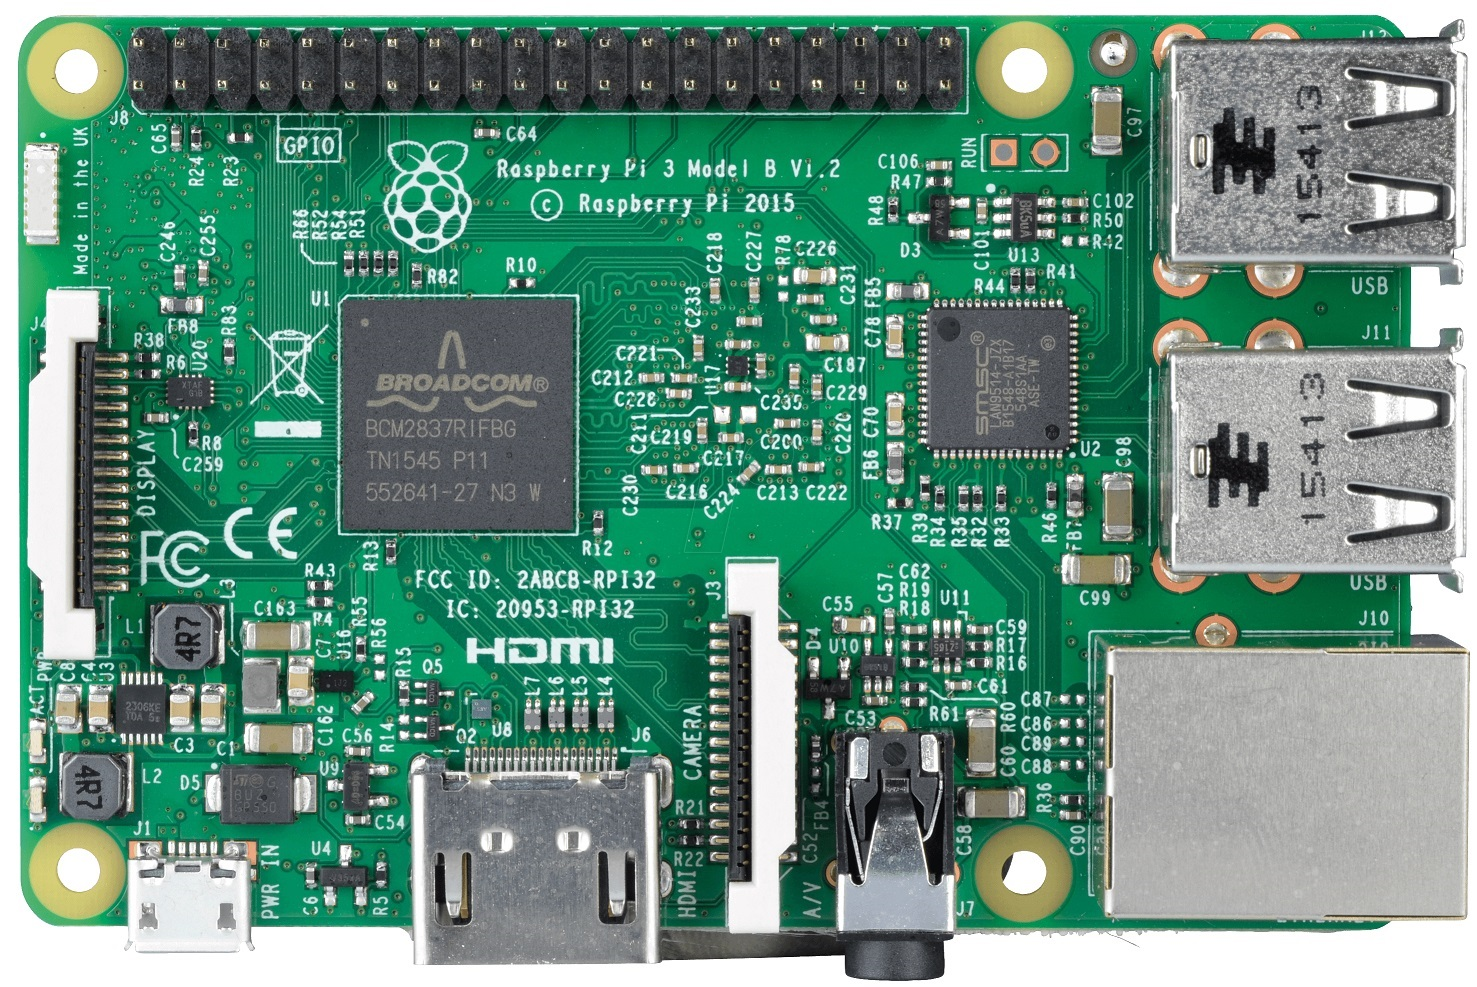
\includegraphics[width=50mm]{pics/rpi3b.jpg}
   	\caption[Raspberry Pi Modelo 3 b]{Raspberry Pi Modelo 3 b}
   \label{figure2.1}
\end{figure}

\subsubsection{}


\subsubsection{Especificaciones}

\begin{itemize}
  \item Chipset Broadcom BCM2387
  \item 1,2 GHz de cuatro núcleos ARM Cortex-A53
  \item 1 GB LPDDR2
  \item Ethernet socket Ethernet 10/100 BaseT
  \item 802.11 LAN inalámbrica
  \item HDMI rev 1.3 y 1.4
  \item USB 4x Conector USB 2.0
  \item Conector GPIO
\end{itemize}

\subsubsection{Límites térmicos}

Uno de los mayores problemas de utilizar Raspberry Pi para el proyecto es que crecen de elementos de disipación de calor propios integrados en la placa, lo que hace que sea especialmente sensible a las altas temperaturas. Bajo una situación de poco estrés mantiene unos rangos de temperatura bastánte estables, sobre los cuarenta grados ºC, pero bajo condiciones de mucha carga de trabajo el aumento de la temperatura es bastánte elevado, llegando a su punto crítico sobre temperaturas cercanas a los ochenta grados ºC, condiciones en las cuales, por seguridad, se produce un apagado súbito del sistema. En la figura \ref{figure2.8} se puede apreciar un procesador con sobre la temperatura crítica de apagado.

\begin{figure}[H]
	\centering
  	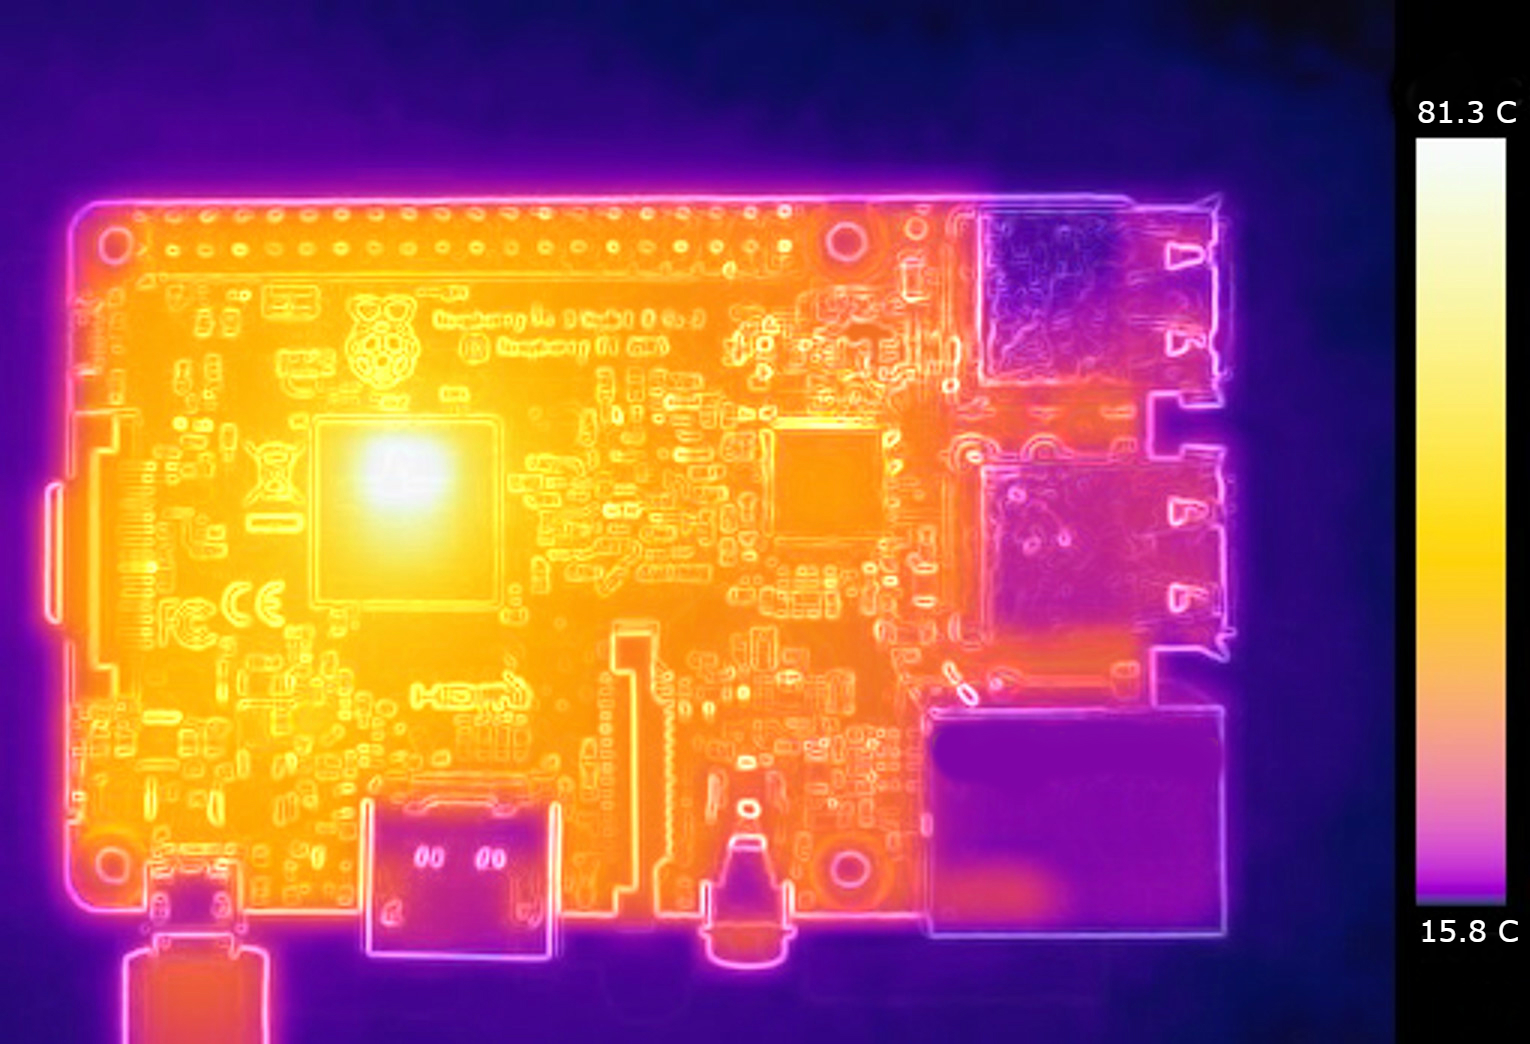
\includegraphics[width=60mm]{pics/pi_3_thermal.jpg}
   	\caption[Captura Térmica]{Límite térmico de la Raspberry}
   \label{figure2.8}
\end{figure}

Esto afecta principalmente a la memoria, controlador de Ethernet y los procesadores.

Debido a la disposición de las tarjetas en forma de columna, existe una gran proximidad entre ellas, lo que hace que aquellas que se encuentren el las partes mas centrales de la estructura estén expuestas a un efecto de tubo de calor proviniente de los nodos que se encuentran próximos a ellas, por esto es necesario disponer de un buen método de disipación de calor, a fin de evitar el sobrecalentamiento del sistema. La disposición y soluciones aportadas a este problema se describen mas ampliamente en el capítulo \ref{ch:capitulo4.tex}.

\subsubsection{Disipadores de calor}

Una de las soluciones aportadas para resolver el problema que se acaba de describir es incluir disipadores de calor sobre el procesador, memoria y controlador Ethernet.

\begin{figure}[H]
	\centering
  	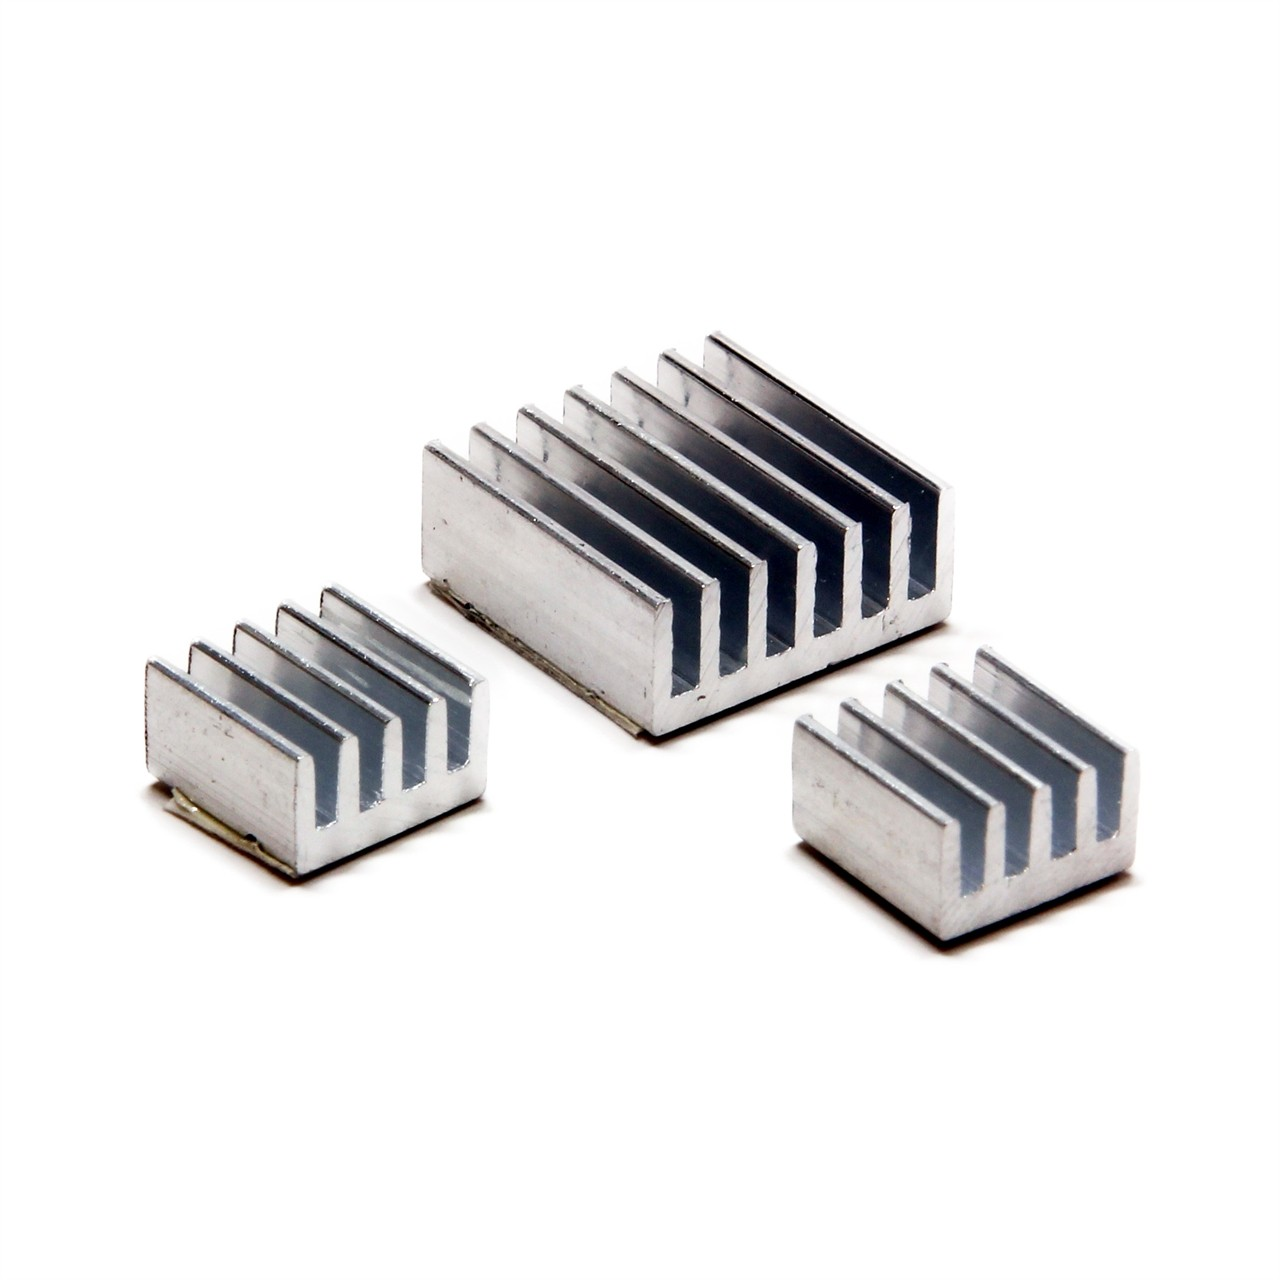
\includegraphics[width=50mm]{pics/disipadores.jpg}
   	\caption[Disipadores ]{Disipadores}
   \label{figure2.8}
\end{figure}

Estos tiene un precio muy reducido y como veremos más adelante, aunque por si solos no suponen una gran mejora, aproximadamente unos dos o tres grados ºC menos que un nodo que no disponga de ellos, con una buena ventilación ofrecen una mejora realmente notoria.

\subsection{Conversor USB 3.0 a Ethernet}

Raspberry 3 modelo B sólo posee un puerto Ethernet, nuestro nodo maestro necesita disponer de un puerto dedicado para cada una de sus conexiones con el front-end y el back-end. Ete dispositivo permite ampliar el número de puertos Ethernet para solucionar dicho problema 

\begin{figure}[H]
	\centering
  	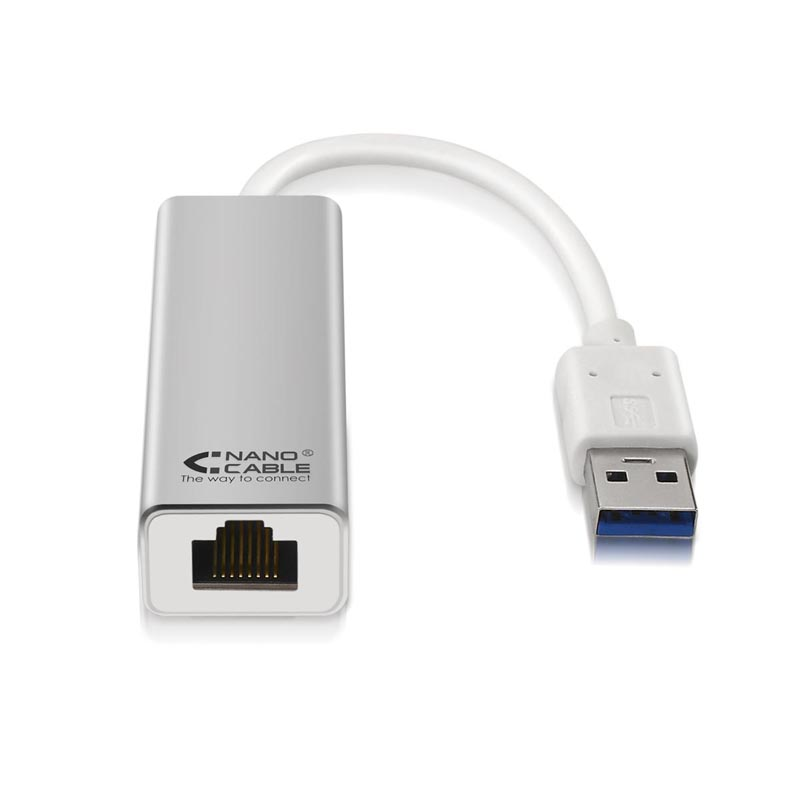
\includegraphics[width=60mm]{pics/ethernetUSB.jpg}
   	\caption[Conversor USB 3.0 a Ethernet]{Conversor USB 3.0 a Ethernet}
   \label{figure2.3}
\end{figure}

\subsubsection{Especificaciones}

\begin{itemize}
  \item Conexión USB 3.0
  \item Compatible con IEEE 802.3, 802.3u y 802.3ab
  \item Chipset RTL8153
  \item Velocidad de transferencia de datos: 10, 100, 1000 Mbps
  \item Detección de crossover y corrección automática
\end{itemize}

Uno de los factores destacables de este componente es que sí puede alcanzar una tasa de transferencia de 1000 Mbps, a diferencia del puerto Ethernet instalado en la Raspberry Pi, esto permite disponer de una mayor velocidad de cara al front-end, permitiendo unas comunicaciones mas fluidas con el exterior del cluster. 

\subsection{Tarjeta microSD SanDisk}

Raspberry Pi no dispone de almacenamiento en disco, en vez de eso dispone de una ranura microSD en la cual viene instalado el sistema operativo. La capacidad de las tarjetas es un factor importante a tener en cuenta ya que la instalación del sistema operativo en tarjetas de un tamaño superior a los 32 Gigabytes requiere de un software específico, haciendo que la instalación sea mas compleja y, como hemos podido comprobar, no es soportada por todas las versiones de Debian Jessie disponibles en el repositorio oficial de raspberypi.org.

\begin{figure}[H]
	\centering
  	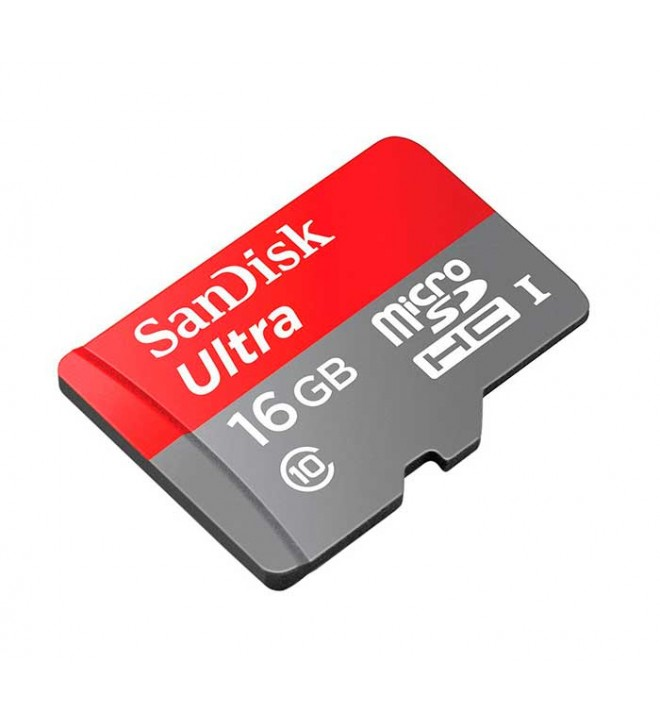
\includegraphics[width=40mm]{pics/sd.jpg}
   	\caption[microSD SanDisk]{microSD SanDisk}
   \label{figure2.2}
\end{figure}

Debido a que el sistema al completo no supera los 11 Gigabytes tanto en los nodos esclavos como en el maestro decidimos usar tarjetas de 16 Gigabytes para todos los nodos de la red, de esta forma reducimos se reduce el gasto y evitamos problemas de compatibilidad entre algunas versiones de Debian Jessie.

\subsection{Switch D-LINK DGS-1008D}

La elección del switch es importante ya que limita el número de nodos que puede haber dentro del cluster, esto, junto con los  cables de alimentación, tiene una influencia directa sobre el tamaño del contenedor, así como la escalabilidad del cluster. Por otro lado, el reducido presupuesto no nos ha permitido disponer de más nodos de cómputo, debido a todos estos parámetros decidimos trabajar con un switch de ocho puertos, lo que permite disponer de hasta siete nodos de cómputo, ya que una de las entradas del mismo sirve como puente entre módulos, permitiendo, en caso de que se requiera, aumentar el número de nodos.

\begin{figure}[H]
	\centering
  	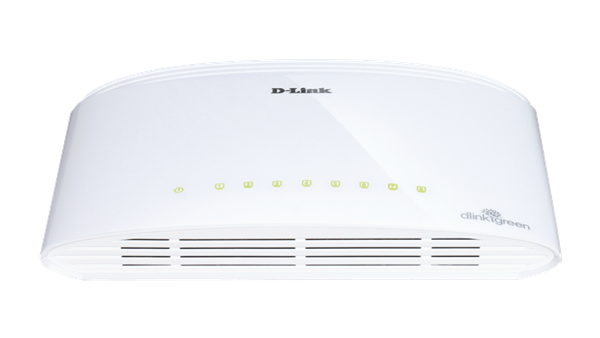
\includegraphics[width=60mm]{pics/DGS_1008DSwitch8.png}
   	\caption[Switch D-LINK DGS-1008D]{Switch D-LINK DGS-1008D}
   \label{figure2.2}
\end{figure}

\subsubsection{Especificaciones}

\begin{itemize}
  \item 8 Puertos Ethernet 1000/100/10 Mbps
  \item Velocidad de transferencia: 2000 Mbps full duplex
\end{itemize}

Como podemos ver en las especificaciones este modelo permite alcanzar una velocidad de hasta 1000 Mbps, sin embargo el modelo de Raspberry Pi utilizado está limitado a 100 Mbps. En la versión mas reciente de Raspberry (Modelo B+), este límite sigue vigente, sin embargo se espera que posteriores modelos alcancen esta velocidad, lo que mejoraría las comunicaciones dentro del equipo. 



\subsection{Ventiladores}
\subsubsection{Especificaciones}

\begin{figure}[H]
	\centering
  	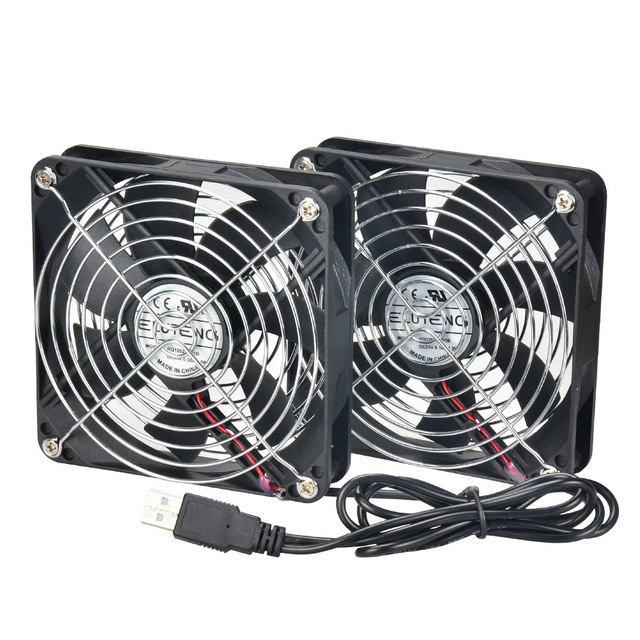
\includegraphics[width=60mm]{pics/fan120.png}
   	\caption[Ventiladores USB]{Ventiladores USB}
   \label{figure2.4}
\end{figure}

\subsection{Cargador USB}

\subsubsection{Especificaciones}
\begin{figure}[H]
	\centering
  	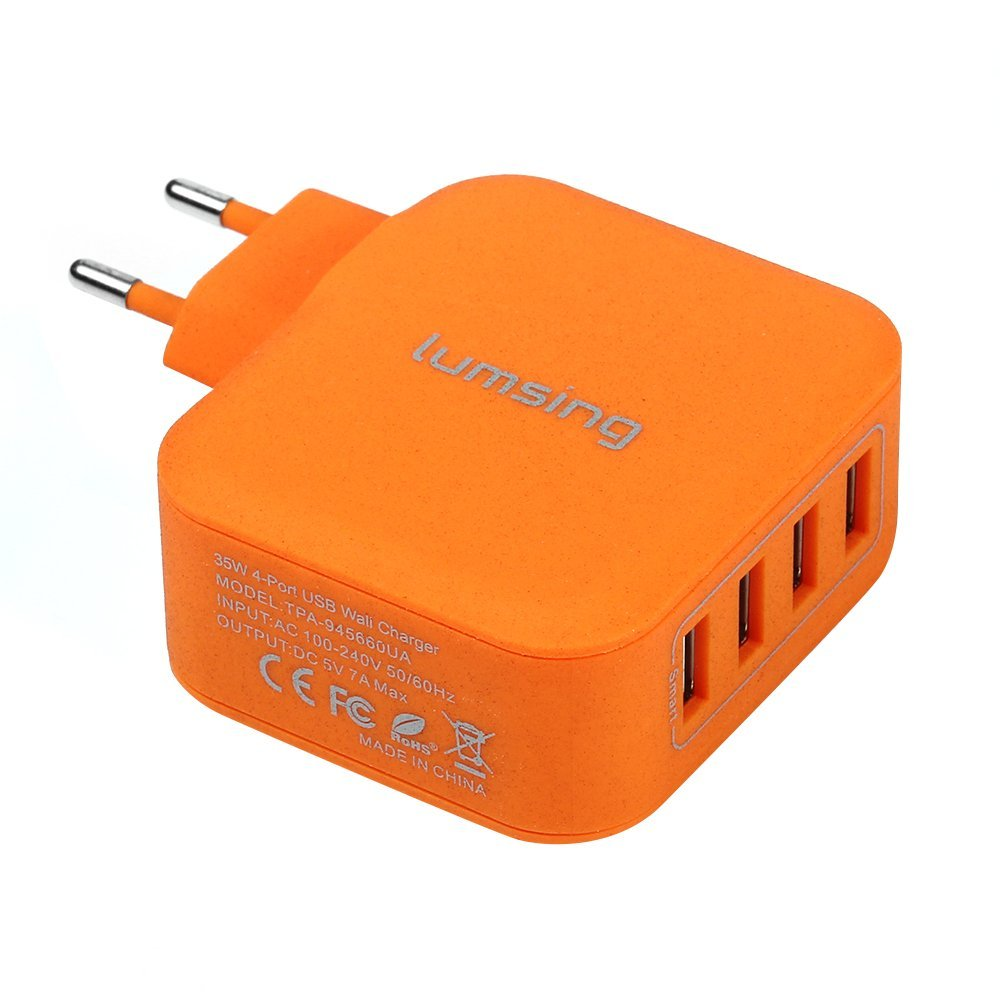
\includegraphics[width=60mm]{pics/cargadorUSB.jpg}
   	\caption[Cargador USB]{Cargador USB}
   \label{figure2.5}
\end{figure}

\subsubsection{Falta de energía}

La raspberry necesita de tres Amperios para poder funcionar, inicialmente el encargado de alimentar al cluster era un Hub de 10 puertos como el de la figura \ref{figure2.7}, tras las primeras pruebas descubrimos que repartía de forma uniforme la energía a todo el sistema y no conseguía llegar a satisfacer(sí, he dicho satisfacer) a ninguna raspberry por separado.//REVISAR


\begin{figure}[H]
	\centering
  	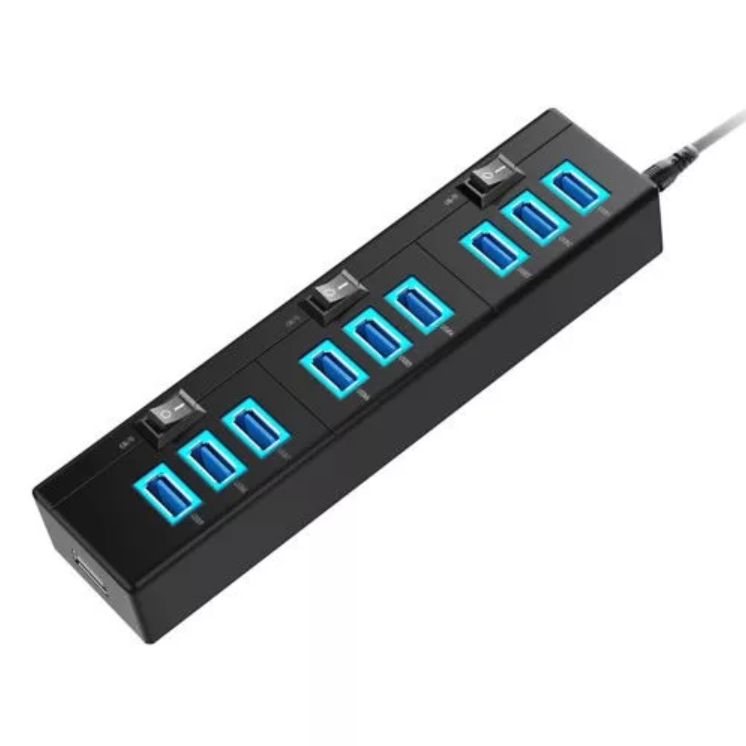
\includegraphics[width=60mm]{pics/Hub.PNG}
   	\caption[Problemas de energía]{Hub Inicial}
   \label{figure2.7}
\end{figure}


La solución a este problema la hallamos en dos cargadores como los de la figura \ref{figure2.5} de cuatro puertos y que reparten de forma eficiente alimentación a tres raspberrys y un ventilador cada uno.
\newpage
\chapter{Configuración del clúster}
\label{ch:capitulo3.tex}

\begin{FraseCelebre}
	\begin{Frase}
		Tenemos que fabricar máquinas que nos permitan seguir fabricando máquinas, porque lo que no va a hacer nunca la máquina es fabricar máquinas
	\end{Frase}
	\begin{Fuente}
	M.Rajoy
	\end{Fuente}
\end{FraseCelebre}

Al lo largo de este capítulo se detallan los pasos necesarios para la correcta configuración del sistema. En cada apartado se especifican los pasos a seguir para la configuración e instalación de los distintos servidores y software necesarios. 

\section{Virtualización del sistema}
\label{makereference3.1}
\paragraph{}

Debido a la gran cantidad de componentes necesarios para el desarrollo del proyecto, la necesidad de realizar el montaje y desmontaje de forma manual de estos y la dificultad en el acceso y configuración de cada uno de los nodos que lo componen decidimos realizar una virtualización del sistema para minimizar los problemas antes descritos. Así, al disponer de un entorno virtual, el cual, replica el clúster real, se minimiza el tiempo necesario para la configuración de los distintos servicios y servidores del sistema operativo y sirve, a su vez, como banco de pruebas para el desarrollo de software.

Para ello, hemos utilizamos \textit{VMware workstation 12} como plataforma de software de virtualización y una \textbf{imagen} de Raspbian basada en \textit{Debian Stretch} , la cual se encuentra disponible en la página oficial de Raspberry Pi\footnote{\url{http://downloads.raspberrypi.org/raspbian/images/}}. Aunque el sistema del clúster parte de una versión diferente de Debian, el sistema de carpetas y, sobre todo, la instalación de \textbf{SIMCAN}, es similar al del entorno real.

En el repositorio en \textit{Github} existe una réplica del sistema de carpetas tanto para el servidor como para los nodos esclavo. Cada una de las carpetas y ficheros modificados en el sistema durante la configuración del sistema quedan reflejados en el repositorio, disponiendo así de un listado en forma de árbol de todas las configuraciones necesarias para el correcto funcionamiento de este.

\begin{figure}[H]
	\centering
  	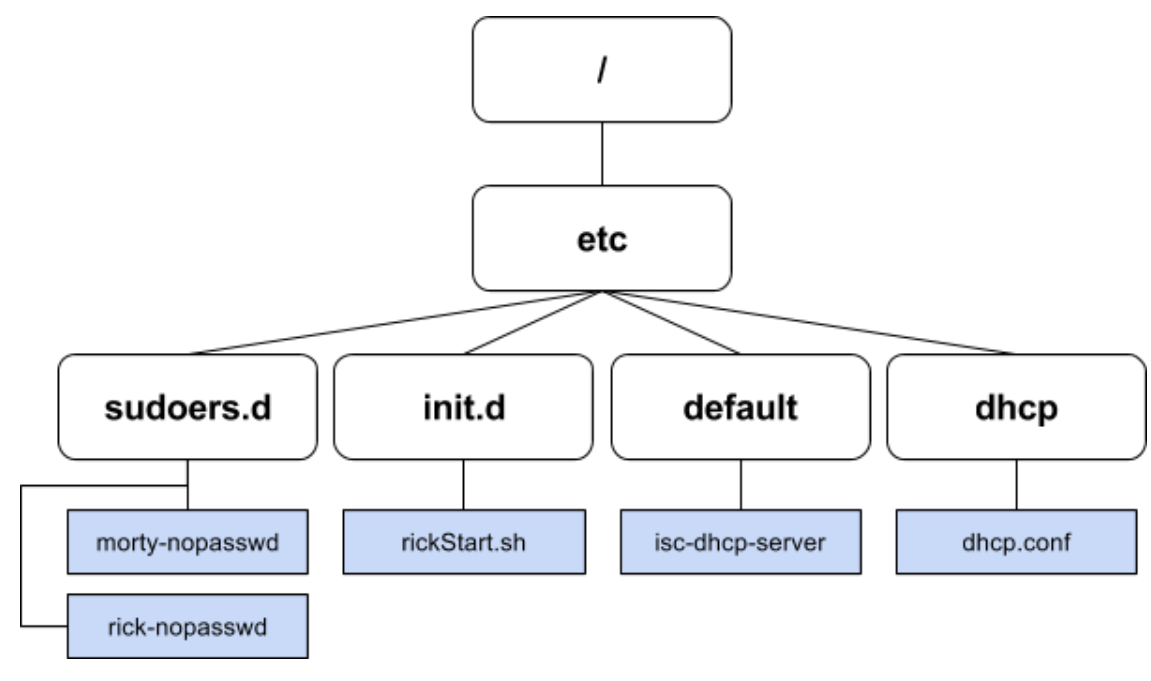
\includegraphics[width=110mm]{pics/sistemadearchivos.PNG}
   	\caption[Sistema de archivos]{Sistema de archivos del repositorio}
   \label{figure3.1}
\end{figure}

\section{Sistema centralizado}
\label{makereference2.6}

Hemos decidido realizar nuestro sistema con una arquitectura de cluster computing centralizado para obtener más rendimiento y paralelizar aplicaciones, de este modo aprovechamos todos los recursos del cluster en su ejecución.

Disponemos de un nodo maestro que contiene el front-end y el back-end y realiza el envío de las peticiones a los esclavos, es escalable pudiendo incorporar nuevos nodos a la red, además ofrece una mayor seguridad sobre los sistemas descentralizados ya que todo el procesamiento es controlado a través de una localización central.

\begin{figure}[H]
	\centering
  	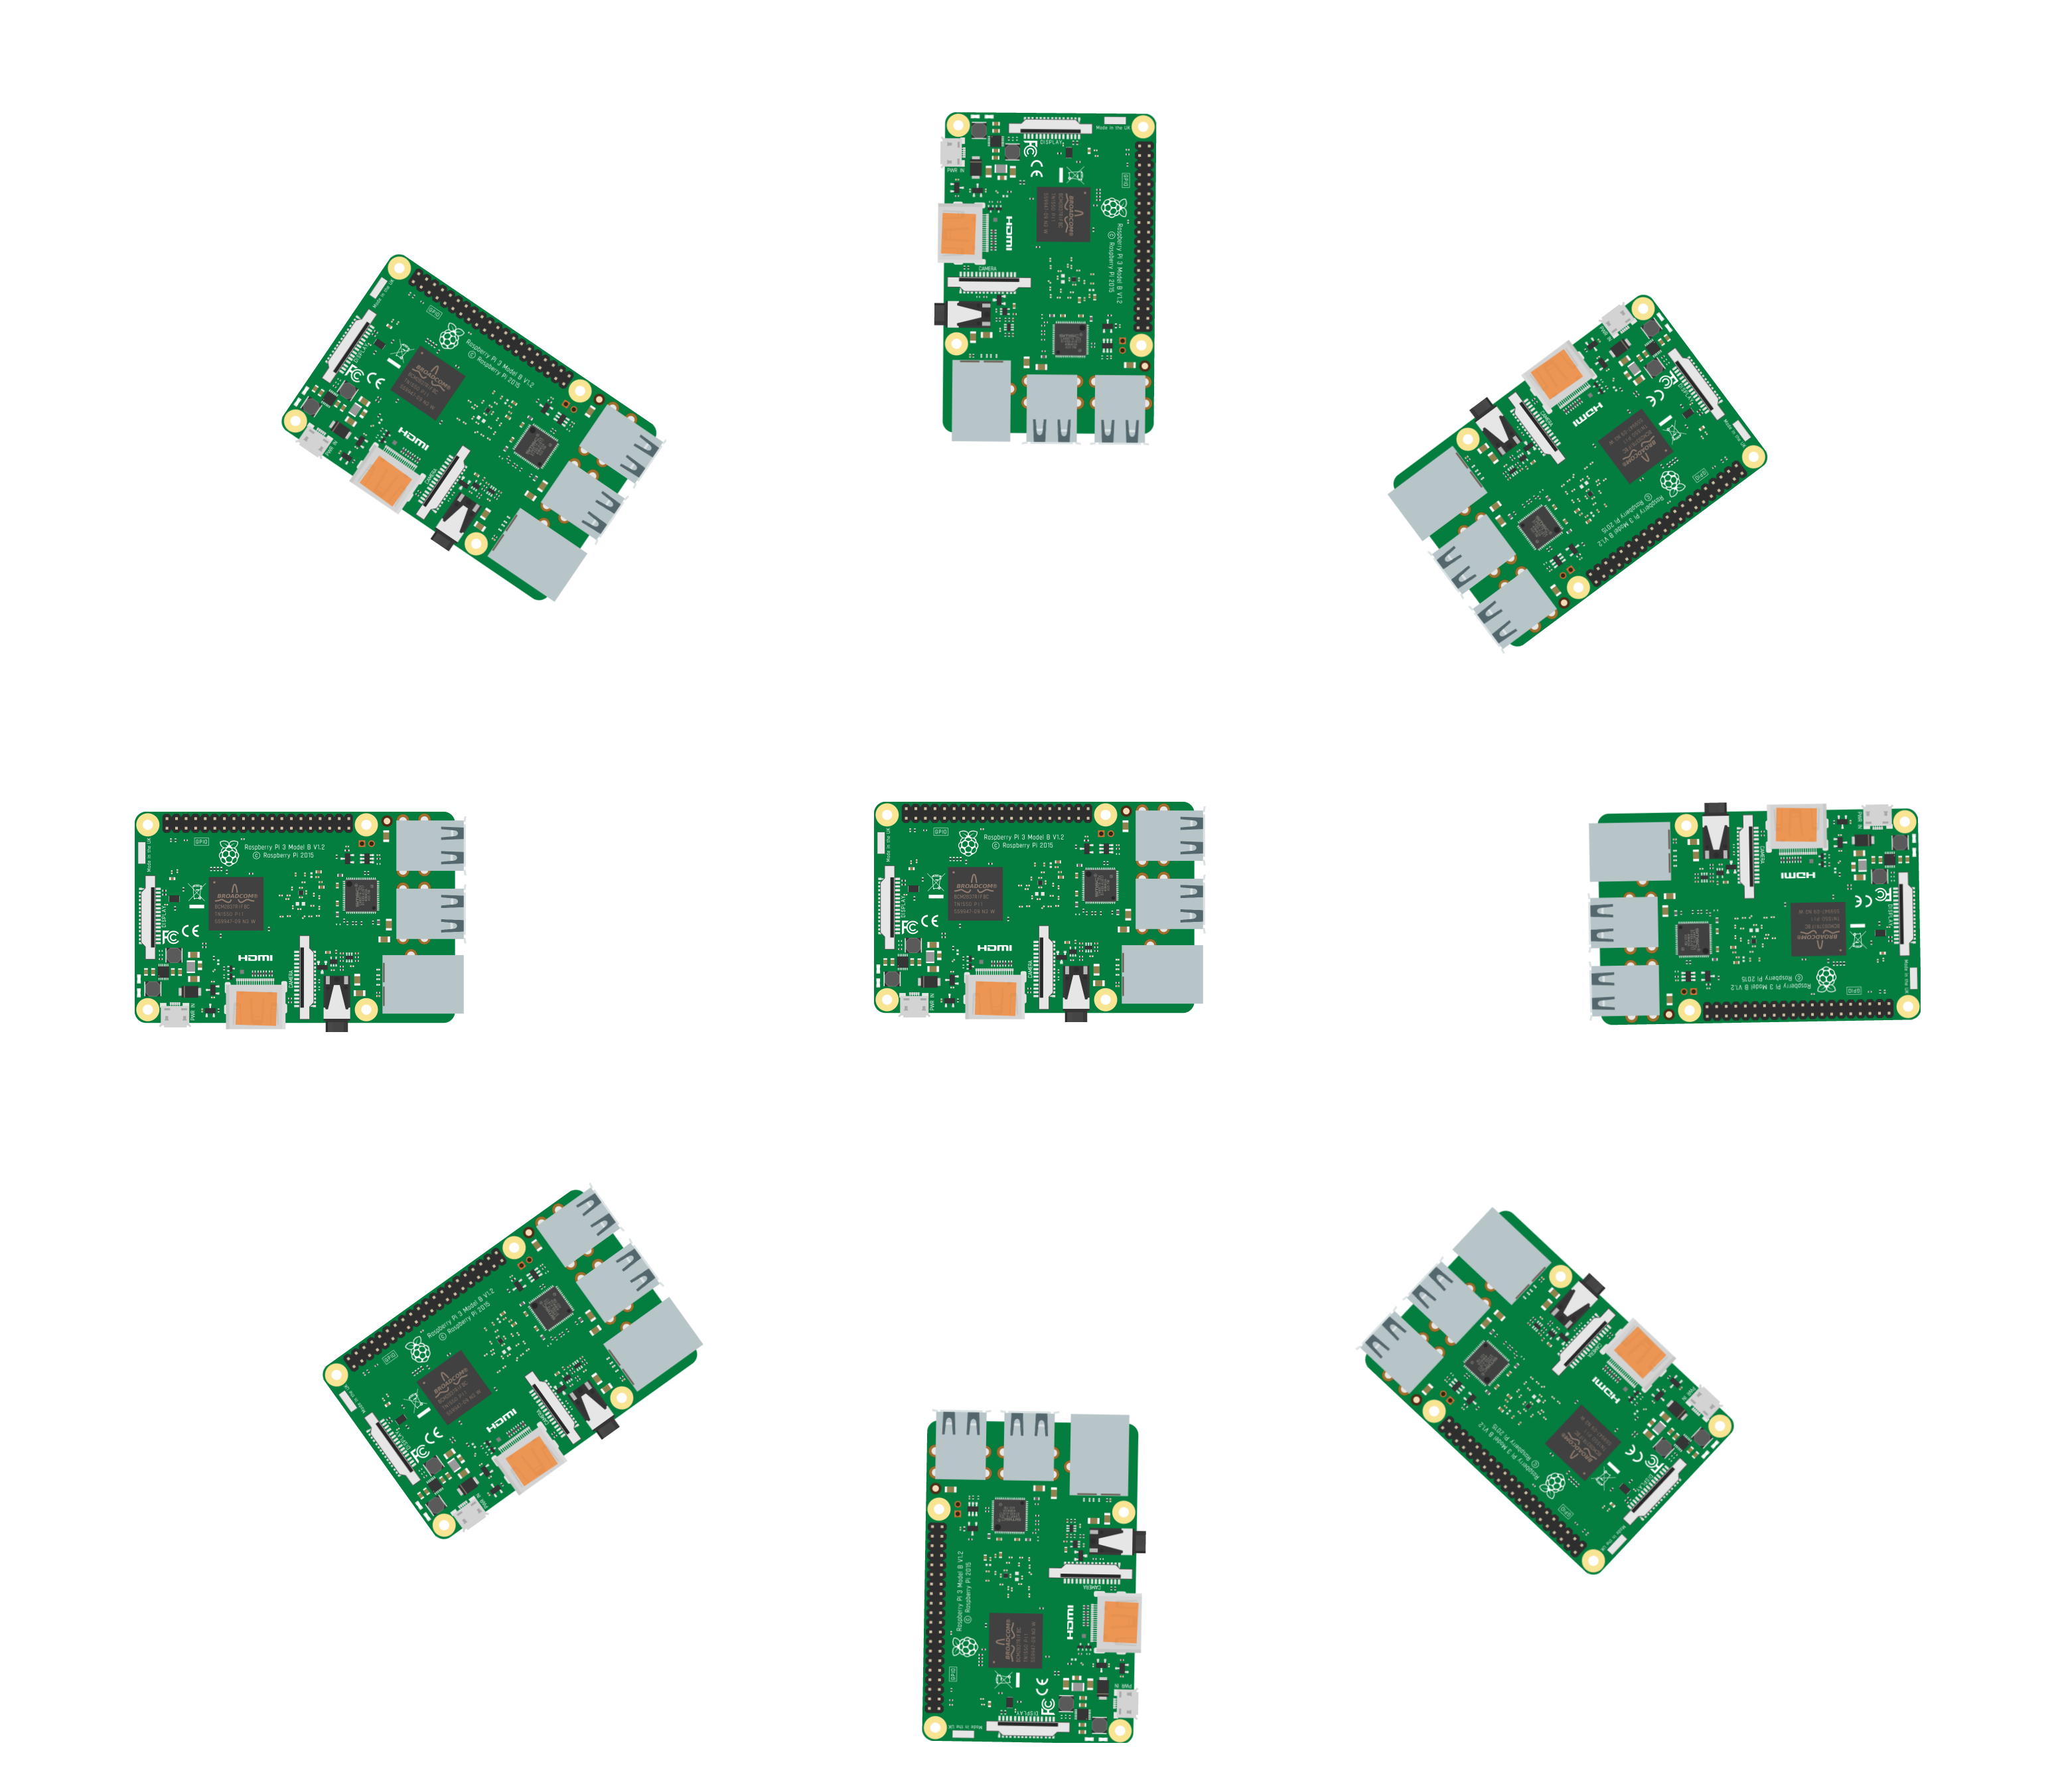
\includegraphics[width=100mm]{pics/centralizado.png}
   	\caption[Sistema centralizado]{Sistema centralizado}
   \label{figure2.6}
\end{figure}

\section{Arquitectura del Clúster}
\label{makereference3.3}
\paragraph{}

El clúster está dividido en dos partes diferenciadas. Por un lado, el \textit{front-end}, servidor, nodo del clúster que tiene instalado el software de \textbf{SIMCAN}, además de ofrecer los servicios de \textbf{NFS}, \textbf{DHCP} y \textbf{SSH} entre otros nodos como muestra la figura \ref{figure3.2}. Además, el punto de comunicación con el exterior, por ello dispone de una tarjeta de red adicional.

\begin{figure}[H]
	\centering
  	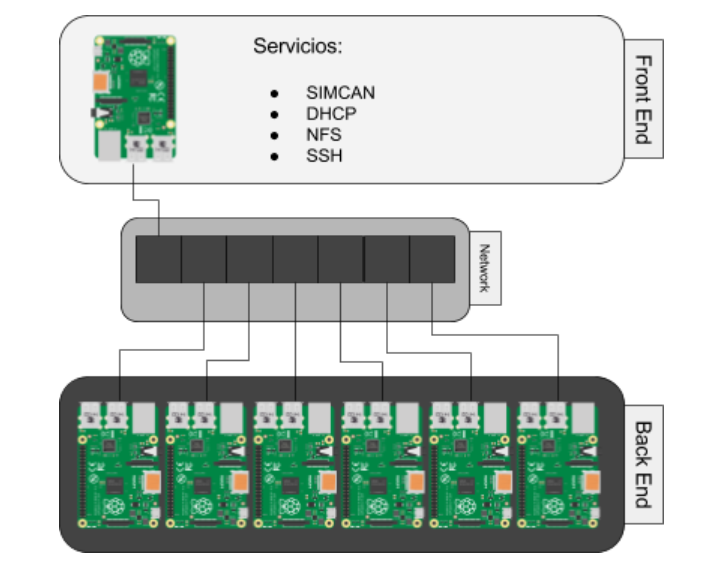
\includegraphics[width=90mm]{pics/servidores.PNG}
   	\caption[Esquema]{Esquema del sistema}
   \label{figure3.2}
\end{figure}

Por otro lado, en el \textit{back-end}, disponemos de varios nodos esclavo que disponen únicamente del sistema Debian Jessie, así como de bibliotecas necesarias para realizar las operaciones de cómputo.

\section{Configuración de la red}
\label{makereference3.4}
\paragraph{}

La configuración de la red se realiza mendiante DHCP, en este caso utilizaremos......

La red en la que trabajamos es la \textit{172.16.111.0/24}. El front end tiene asignada la dirección \textit{172.16.111.1/24}, y ejerce de servidor sobre el resto de nodos, encargándose del reparto de direcciones, como se muestra en la figura \ref{figure3.3}.

\begin{figure}[H]
	\centering
  	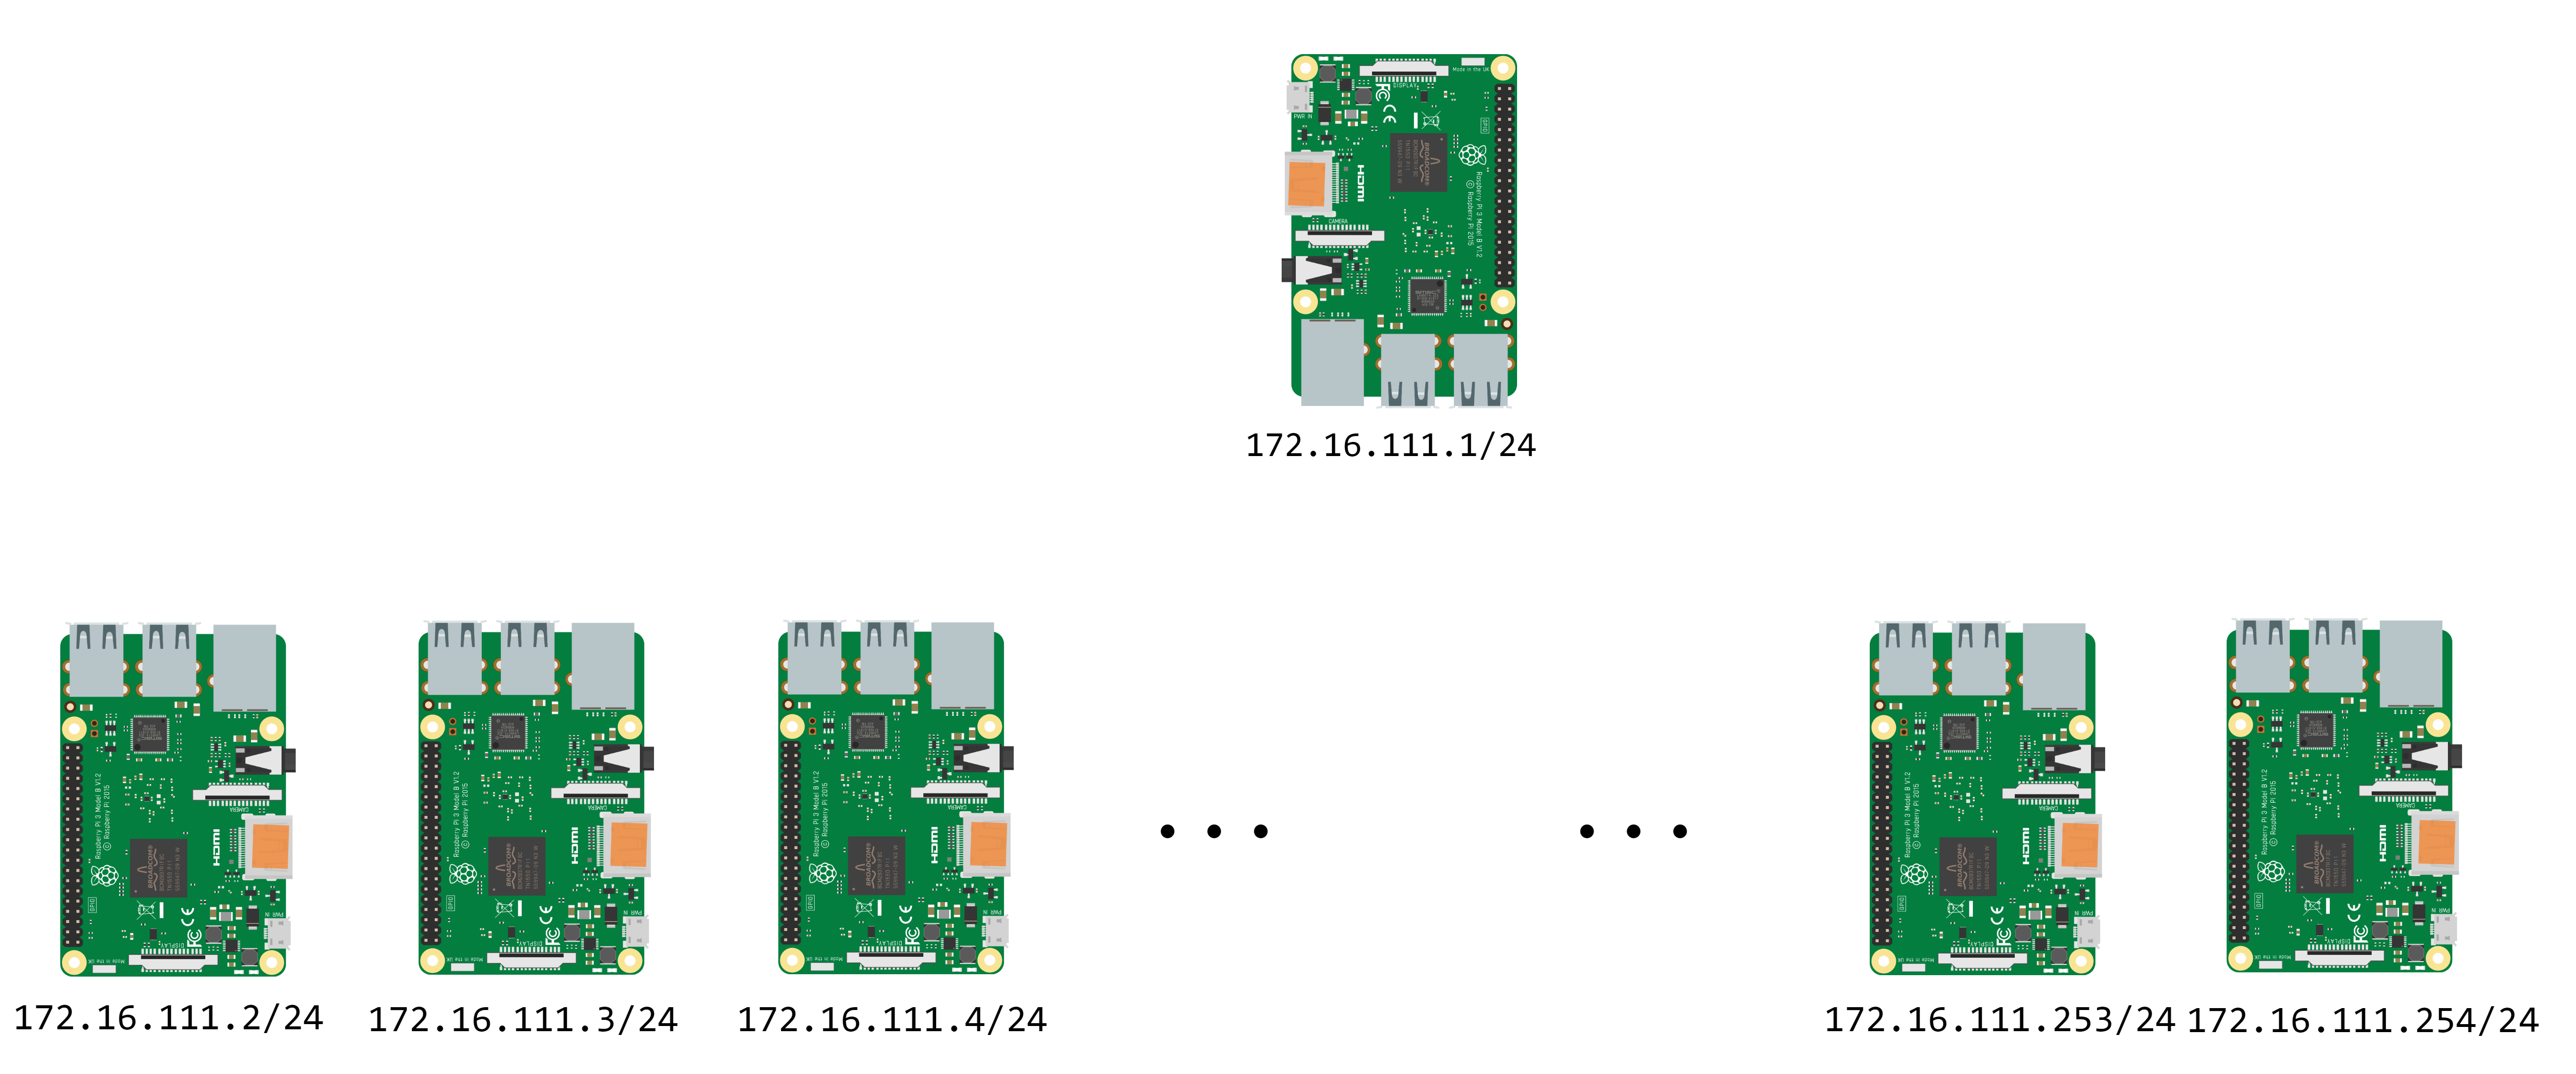
\includegraphics[width=120mm]{pics/dhcpdos.png}
   	\caption[Servidor DHCP]{Servidor DHCP}
   \label{figure3.3}
\end{figure}

Gracias al uso del protocolo \textbf{DHCP} evitamos tener que asignar manualmente direcciones a todos los nodos, sin embargo, es más útil en la práctica que cada uno de los nodos disponga de la misma dirección el máximo tiempo posible.

¿¿Por qué??

Para ello, en el fichero \textbf{/etc/dhcp/dhcpd.conf}, hemos establecido el parámetro \textbf{default-lease-time} que determina el tiempo de concesión de que el servidor asigna a cada nodo en su máximo valor. El tiempo por defecto (7776000 expresado en segundos) será de noventa días.

\begin{lstlisting}[language=c,frame=single,numbers=none]
      ...
      default-lease-time	7776000;
      ...
\end{lstlisting}

Los servicios ofrecidos por el nodo maestro de cara al \textit{front-end} están disponibles a través de su segunda tarjeta de red, configurada para obtener una dirección IP desde un \textbf{ISP}.

\subsection{Configuración de DHCP}
\paragraph{}

Instalación de paquetes en el servidor

\begin{lstlisting}[language=c,frame=single,numbers=none]
  1	sudo apt-get update
  2	sudo apt-get install isc-dhcp-server
\end{lstlisting}

Editar fichero \textbf{/etc/default/isc-dchp-server}

\begin{lstlisting}[language=c,frame=single,numbers=none]
  3	sudo nano /etc/default/isc-dchp-server
  4	INTERFACES = eth0
\end{lstlisting}

Editar fichero \textbf{/etc/network/interfaces}

\begin{lstlisting}[language=c,frame=single,numbers=none]
  5	nano /etc/network/interfaces
  6	source-directory /etc/network/interfaces.d

  auto eth0	
  iface eth0 inet static
  address 172.16.111.106
  netmask 255.255.255.0
  network 192.168.100.0
  gateway 172.16.111.105

  allow-hotplug wlan0
  iface wlan0 inet manual
      wpa-conf /etc/wpa_supplicant/wpa_supplicant.conf

  allow-hotplug wlan1
  iface wlan1 inet manual
      wpa-conf /etc/wpa_supplicant/wpa_supplicant.conf
\end{lstlisting}

Editar fichero de configuración \textbf{/etc/dhcp/dhcpd.conf}

Incluir la siguiente configuración al final del fichero:
\begin{lstlisting}[language=c,frame=single,numbers=none]
  subnet 172.16.111.0 netmask 255.255.255.0{
      range 172.16.111.106	172.16.111.255;
      option domain-name-servers 8.8.8.8, 4.4.4.4;
      option routers		172.16.111.105;
  }
  host Rick{
      hardware ethernet <dir MAC del servidor>
      fixed-address 172.16.111.110;
  }
\end{lstlisting}

Activación de la red eth0 y reinicio

\begin{lstlisting}[language=c,frame=single,numbers=none]
  7	sudo ifconfig eth0 up
  8	sudo reboot now 
\end{lstlisting}

Arranque del servicio DHCP

\begin{lstlisting}[language=c,frame=single,numbers=none]
  9	sudo /usr/sbin/dhcpd
\end{lstlisting}

Comprobación del correcto funcionamiento del sistema

\begin{lstlisting}[language=c,frame=single,numbers=none]
  10	ps -ef | grep dhcpd
\end{lstlisting}

Opcionalmente se pueden mostrar las máquinas conectadas al servicio mediante la orden

\begin{lstlisting}[language=c,frame=single,numbers=none]
  11	cat /var/lib/dhcp/dhcp.leases 
\end{lstlisting}

\subsection{Network File System (NFS)}
\label{makereference3.5}
\paragraph{}

Como se destacaba anteriormente, el front-end es el único que dispone de una versión de \textbf{SIMCAN} instalada, con esto se evitan problemas de versiones y es mas sencillo realizar actualizaciones, esta configuración ofrece la posibilidad de que la labor del los nodos esclavo sea únicamente la de realizar el procesamiento de datos. Mediante \textbf{NFS}, el nodo servidor comparte su carpeta /home/ durante el arranque del sistema. De esta forma, el resto de nodos esclavo realizan el montaje de este directorio compartido en red en su propio directorio /home/, creando así un único punto de acceso compartido en red del que se pueden extraer los ejecutables sin la necesidad de disponer de \textbf{SIMCAN} instalado. El front-end se encarga de realizar la compilación los ficheros \textit{.ned} y pone a disposición del resto de nodos los ejecutables.

Es necesario que todos los nodos de la red tengan un mismo usuario común para conseguir una correcta sincronización, de igual manera hay que mantener un estricto control de los permisos de cada uno de los nodos esclavo tanto a nivel interno como de cara al servidor.

\subsection{Instalación de NFS}
\paragraph{}

PARRAFO DE INTRODUCCION.....

Instalar paquetes en el servidor

\begin{lstlisting}[language=c,frame=single,numbers=none]
  1	sudo apt-get update
  2	sudo apt-get install nfs-kernel-server
\end{lstlisting}

Editar fichero de configuración \textbf{/etc/exports} en servidor
\begin{lstlisting}[language=c,frame=single,numbers=none]
	Incluir al final del fichero el directorio a compartir:
	Ruta de carpeta
	Dirección IP de máquina destino / permisos

	Ejemplo: /home/morty 172.16.111.0/24(rw,no_subtree_check)
\end{lstlisting}

Instalación de paquetes en el cliente
\begin{lstlisting}[language=c,frame=single,numbers=none]
  Instalados por defecto en raspBian
  3	sudo apt-get update
  4	sudo apt-get install build-essential gcc g++ bison flex perl  tcl-dev tk-dev libxml2-dev zlib1g-dev default-jre doxygen graphviz libwebkitgtk-1.0-0 openmpi-bin libopenmpi-dev libpcap-dev
\end{lstlisting}

Ejecutar cambios realizados en el servidor

\begin{lstlisting}[language=c,frame=single,numbers=none]
  5	sudo exportfs -a
  6	sudo mount 172.16.111.x:/home/morty /home/morty
      172.16.111.x es la dirección ip de servidor
\end{lstlisting}

Reiniciar servicios 
\begin{lstlisting}[language=c,frame=single,numbers=none]
  7	sudo /etc/init.d/rpcbind restart
  8	sudo /etc/init.d/nfs-kernel-server restart
\end{lstlisting}

Es necesaria una configuración extra para el funcionamiento de NFS, pare ello modificamos permisos de la maquina cliente:
\begin{enumerate}

\item El usuario de la máquina ha de ser sudoer. La carpeta compartida debe tener permisos de lectura, escritura y ejecución \textbf{(LWX)}:

\begin{lstlisting}[language=c,frame=single,numbers=none]
    chmod -R 0777 scenario
\end{lstlisting}

\end{enumerate}
\subsection{Creación y ejecución del servidor NFS como un  \textit{daemon} del sistema}
\paragraph{}

Para evitar tener que realizar el arranque del servidor de forma manual es recomendable crear un \textit{daemon} e incluirlo en el directorio \textbf{/etc/init.d} para que se ejecute con el arranque del sistema de forma automática.

Contenido del script:

\begin{lstlisting}[language=c,frame=single,numbers=none]
	#!/bin/bash
	### BEGIN INIT INFO
	# Provides:		M.Romero && D.Quinones
	# Required-start:	$syslog
	# Required-stop:	$syslog
	# Default-Start:	2 3 4 5
	# Default-Stop:		0 1 6
	# Short-Description:	Inicialización de servicios nfs
	# Description:	
	### END INIT INFO

	sudo exportfs -a
	sudo /etc/init.d/rpcbind restart
	sudo /etc/init.d/nfs-kernel-server restart

  # El orden de estos últimos comandos es esencial
\end{lstlisting}

El siguiente cuadro muestra los pasos a seguir para lanzar el script como un \textit{daemon} del sistema:

\begin{lstlisting}[language=c,frame=single,numbers=none]
  10	chmod +x nombre_del_script.sh
  11	cp nombre_del_script.sh /etc/init.d/
  12	cd /etc/init.d
  13	update-rc.d nombre_del_script.sh defaults
\end{lstlisting}

\section{Instalación de Omnet, Inet y SIMCAN}
\label{makereference3.6}
\paragraph{}
Antes de poder instalar el software \textbf{SIMCAN} es necesario realizar la instalación previa framework \textbf{Omnet++} en su versión 4.6. Además de la suite \textbf{Inet}, que implementa modelos de código abierto \textbf{Omnet++} para redes cableadas, inalámbricas y móviles.

Debido a la baja potencia de la Raspberry, ésta no es capaz de lanzar la aplicación de forma gráfica. Esto supone un problema a la hora de realizar la instalación del software. Es por esto que todas las instalaciones han de realizarse a través del terminal. Esto afecta principalmente a la instalación de \textbf{Inet}, ya que las principales guías de instalación disponibles en las webs oficiales parten siempre del entorno gráfico de \textbf{Omnet++}.

Durante el desarrollo del proyecto se han desarrollado una serie de guías para la instalación y configuración que se desglosarán el el siguiente apartado.

\subsection{Instalación de Omnet}
\paragraph{}

Descargar los \textit{tar.gz}  de Omnet 4.6, Inet, simcan.tar.
Esta última (simcan) incluye las bibliotecas que se necesitan para la compilación.
Copiar los archivos \textit{.tar} de Omnet e Inet en \textbf{/pi} y descomprimir. Desde el directorio \textbf{/pi} ejecuta los siguientes comandos:

\begin{lstlisting}[language=c,frame=single,numbers=none]
  1	sudo apt-get update
  2	sudo apt-get install build-essential gcc g++ bison flex perl  tcl-dev tk-dev libxml2-dev zlib1g-dev default-jre doxygen graphviz libwebkitgtk-1.0-0 openmpi-bin libopenmpi-dev libpcap-dev
  3	sudo apt-get install gnome-color-chooser
  4	cd omnetpp-4.6
  5	. setenv
  6	./configure
  7	make
  * Opcionalmente podemos utilizar el comando make -j 'numero de cores'
  para paralelizar el compilado del proyecto
\end{lstlisting}

\subsection{Instalación de Inet}
\paragraph{}

INCLUIR FRASE DE INTRODUCCIÓN

Crear un directorio nuevo en \textbf{/omnet-4.6} llamado \textit{proyect}, copiar en el directorio \textbf{Inet} descomprimido y ejecutar:

\begin{lstlisting}[language=c,frame=single,numbers=none]
  8	sudo apt-get install libavcodec-dev libavformat-dev
  9	make makefiles
  10	make
  * Opcionalmente podemos utilizar el comando make -j 'numero de cores'
  para paralelizar el compilado del proyecto
\end{lstlisting}

\subsection{Instalación de SIMCAN}
\paragraph{}

Copia el directorio de \textbf{simcan} a \textbf{/projects} y ejecuta los siguientes comandos:

\begin{lstlisting}[language=c,frame=single,numbers=none]
  11	export omnetpp_root=$HOME/morty/omnnetpp-4.6
  12	export INET_HOME=$omnetpp_root/projects/inet
  13	export SIMCAN_HOME=$omnetpp_root/projects/simcan
  14	export LD_LIBRARY_PATH=$omnetpp_root/lib:$LD_LIBRARY_PATH 
  15	export PATH=omnetpp_root/bin:$PATH
  16	make makefiles
  17	make
  * Opcionalmente podemos utilizar el comando make -j 'numero de cores'
  para paralelizar el compilado del proyecto
  Enjoy!
\end{lstlisting}

\subsection{Problemas}
\paragraph{}

\begin{enumerate}

\item No se encuentra el fichero \textbf{TCPCommand\_m.h}
\begin{lstlisting}[language=c,frame=single,numbers=none]
	cp /home/pi/omnetpp-4.6/proyects/inet/src/transport/contract/TCPCommand_m.h /home/pi/omnetpp-4.6/proyects/simcan/src/Messages/TCPCommand_m.h
\end{lstlisting}

\item Error al ejecutar \textbf{run\_simcan}

\begin{lstlisting}[language=c,frame=single,numbers=none]
	chmod +x /simcan/src/run_sincam
\end{lstlisting}

\end{enumerate}


\section{Configuraciones derivadas de la arquitectura}
\label{makereference3.7}
\paragraph{}

Como se ha explicado anteriormente, la arquitectura elegida distribuye la potencia a todos los nodos del clúster desde una misma fuente de alimentación. Debido a la menor cantidad de recursos y servicios que han de ofrecer los nodos esclavo, éstos tienen una carga del sistema ligeramente más rápida que la del nodo maestro. Por ello, se pueden producir problemas de sincronización de servicios, más concretamente, en el montaje de sistemas de ficheros compartidos en red por \textbf{NFS}, el cual es crítico para el funcionamiento general del sistema. Para solucionar este problema se han realizado modificaciones a fin de conseguir acelerar la carga del nodo maestro y ralentizar la del resto.

\subsection{Modificación del GRUB}
\paragraph{}

Una de las soluciones más sencillas para resolver el problema de sincronización consiste en aumentar el tiempo por defecto del \textit{grub} de los nodos esclavo ya que la carga del sistema se produce cuando éste termina. Para ello únicamente hay que modificar la opción \textbf{GRUBTIMEOUT} en el fichero \textbf{/etc/default/grub}. 
En las pruebas realizadas durante la virtualización del sistema se comprobó que estableciendo un retardo de veinticinco segundos era suficiente para que el nodo maestro realizase la carga completa del sistema. Sin embargo, queda por comprobar que en el entorno real esto se sigue produciendo.

Contenido del fichero \textbf{/etc/default/grub} de un nodo esclavo:

\begin{lstlisting}[language=c,frame=single,numbers=none]
  GRUB_DEFAULT=0
  GRUB_TIMEOUT=25
  GRUB_DISTRIBUTOR=`lsb_release -i -s 2> /dev/null || echo Debian`
  GRUB_CMDLINE_LINUX_DEFAULT="quiet splash plymouth.ignore-serial-consoles"
  GRUB_CMDLINE_LINUX=""
\end{lstlisting}

\subsection{Habilitar arranque automático de un usuario}
\paragraph{}

Para modificar el usuario de arranque por defecto es necesario realizar los siguientes cambios en el fichero \textbf{/etc/lightdm/lightdm.conf}
\begin{lstlisting}[language=c,frame=single,numbers=none]
  autologin-user = nombre_de_usuario
\end{lstlisting}

\subsection{Forzar el arranque sin HDMI}
\paragraph{}

En ocasiones \textit{Raspbian Jessie} no realiza la carga del sistema operativo si el conector \textbf{HDMI} no está acoplado en la Raspberry, para forzar el arranque del sistema es necesario modificar el archivo \textbf{/boot/config.txt}

\begin{lstlisting}[language=c,frame=single,numbers=none]
	#Arranque sin HDMI
    hdi_force_hotplug = 1
\end{lstlisting}

\section{Seguridad}
\label{makereference3.8}
\paragraph{}
Por defecto, en las distribuciones de \textit{Debian Jessie} existentes en los repositorios oficiales de raspberry.org existe...
Vienen configurados usuarios por defecto
Root no tiene contraseña
Hay que eliminar a pi como superuser
Sólo dejar morty como superuser en maestro pero no en esclavos

\section{Eliminar usuarios y permisos}
\label{makereference3.9}
\paragraph{}
UID, todos han de tener el mismo, permisos en maestro, esclavo
Inicialización del sistema mediante scripts



\newpage
\chapter{Diseño de Prototipos}
\label{ch:capitulo4.tex}

\begin{FraseCelebre}

\begin{Frase}
		La cosa está muy mal... estoy friendo los huevos con saliva
	\end{Frase}
    
	\begin{Fuente}
	Gregorio Esteban Sánchez
	\end{Fuente}

\end{FraseCelebre}


En este capítulo se muestra el diseño de los distintos modelos que se han generado para el proyecto. Se dispone, para cada uno, una vista en 3D, creada con \textit{OpenScad}, que representa la disposición de los distintos componentes y la dirección de las corrientes de aire generadas por los ventiladores, finalmente, se incluyen capturas del resultado de cada uno de ellos.

\section{Características del modelado}
\label{makereference4.2}
\paragraph{}

Los componentes representados en el modelo en 3D son: el switch de ocho puertos (\textcolor[rgb]{0.16,0.3,0.67}{Azul}), un clúster de Raspberrys formado por siete nodos (\textcolor[rgb]{0.1,0.57,0.2}{Verde}), la base de enchufes (\textcolor[rgb]{0.71,0.28,0.25}{Rojo}) y los ventiladores (\textcolor[rgb]{0.58,0.58,0.58}{Gris}), no se incluyen los cables y conectores conectados a la base y a cada Raspberry.

En cuanto a la disposición de los ventiladores, para cada uno de los modelos, se han realizado diferentes configuraciones, todas ellas destinadas a obtener la corriente de aire más eficiente y la mejor tasa de temperatura cuando los nodos están trabajando a máximo rendimiento. 

Los resultados de estas se muestran en el capítulo \ref{ch:capitulo5.tex}, en donde se verá el comportamiento de cada una con una serie de pruebas destinadas a medir la temperatura ante distintos escenarios.

\section{Modelo 1} 
\label{makereference4.3}
\paragraph{}

En este modelo la distribución de aire se hace con los ventiladores opuestos entre sí, creando una corriente de aire alrededor del rack de Raspberrys que se encuentra frente a ellos. 
 
\begin{figure}[H]
	\centering
  	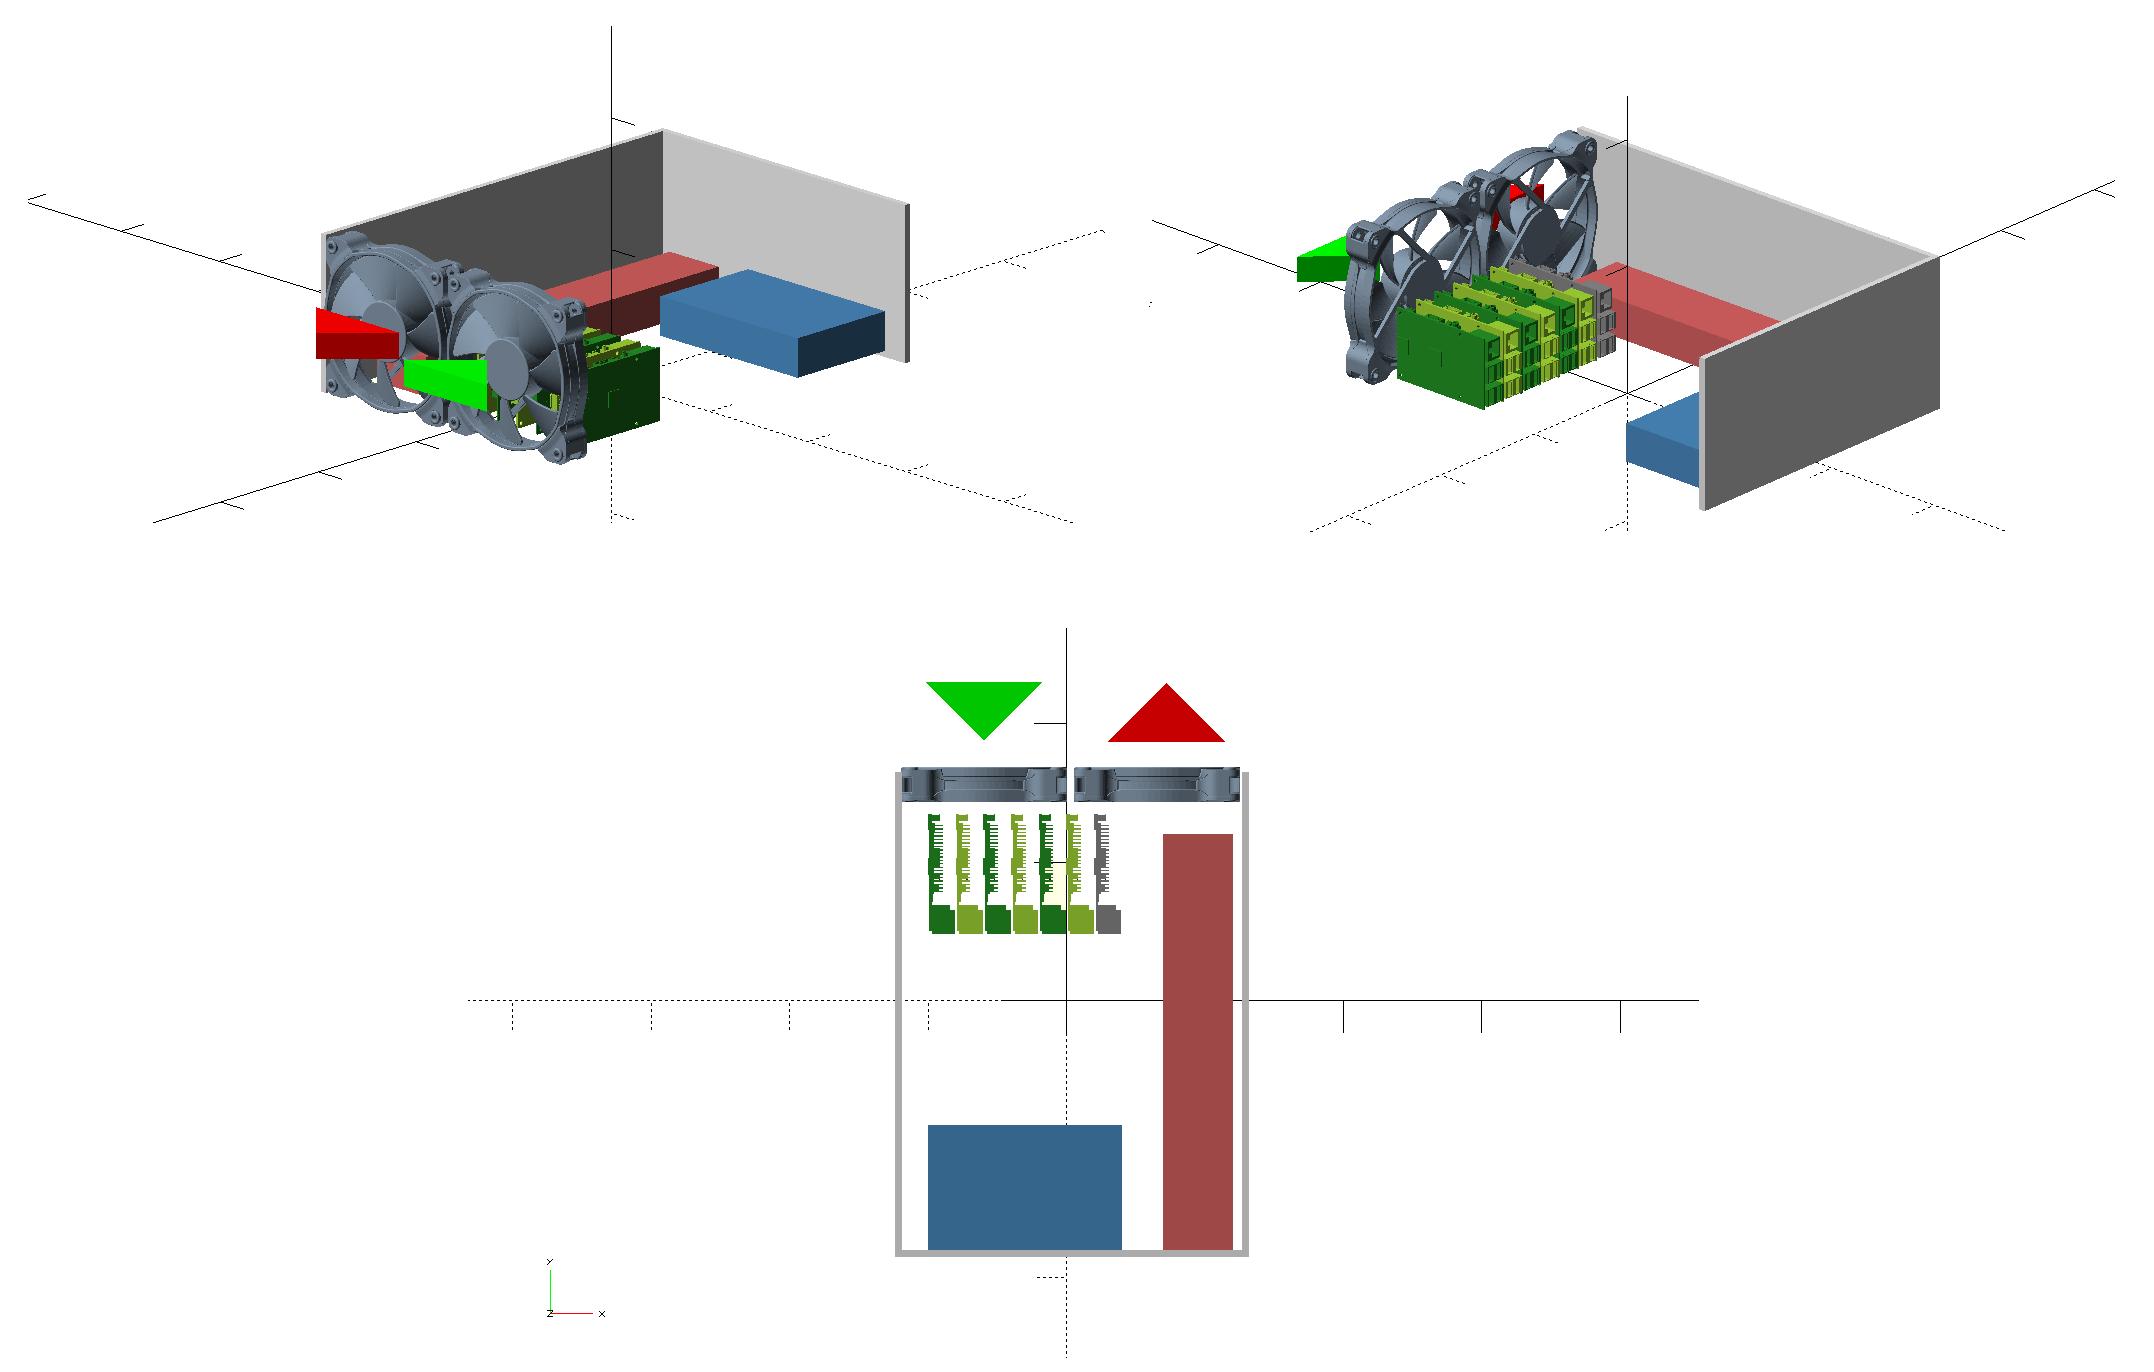
\includegraphics[width=120mm]{Modelos/M1X.png}
   	\caption[Modelo 1 3D]{Modelo 1 3D}
   \label{figure4.1}
\end{figure}

La figura \ref{figure4.1} muestra la vista trasera, delantera y alzada del modelo. La prioridad es obtener una buena distribución de aire, no se ha tenido en cuenta la facilidad para acceder a los componentes.
Para poder acceder a las tarjetas \textbf{SD} de cada Raspberry es necesario mover todo el rack, lo que hace que sea complicado, una solución alternativa sería ofrecer la opción de desacoplar uno de los ventiladores para facilitar el acceso.

\subsection{Resultado}
\paragraph{}

Este modelo tiene un tamaño de 122x123x35 cm y en la captura no se han incluído los cables rj45 que conectan el rack de Raspberrys con el switch.
Podemos observar que los componentes disponen de un espacio muy limitado y que la poca flexibilidad de los cables dificulta el cierre del contenedor.

\begin{figure}[H]
	\centering
  	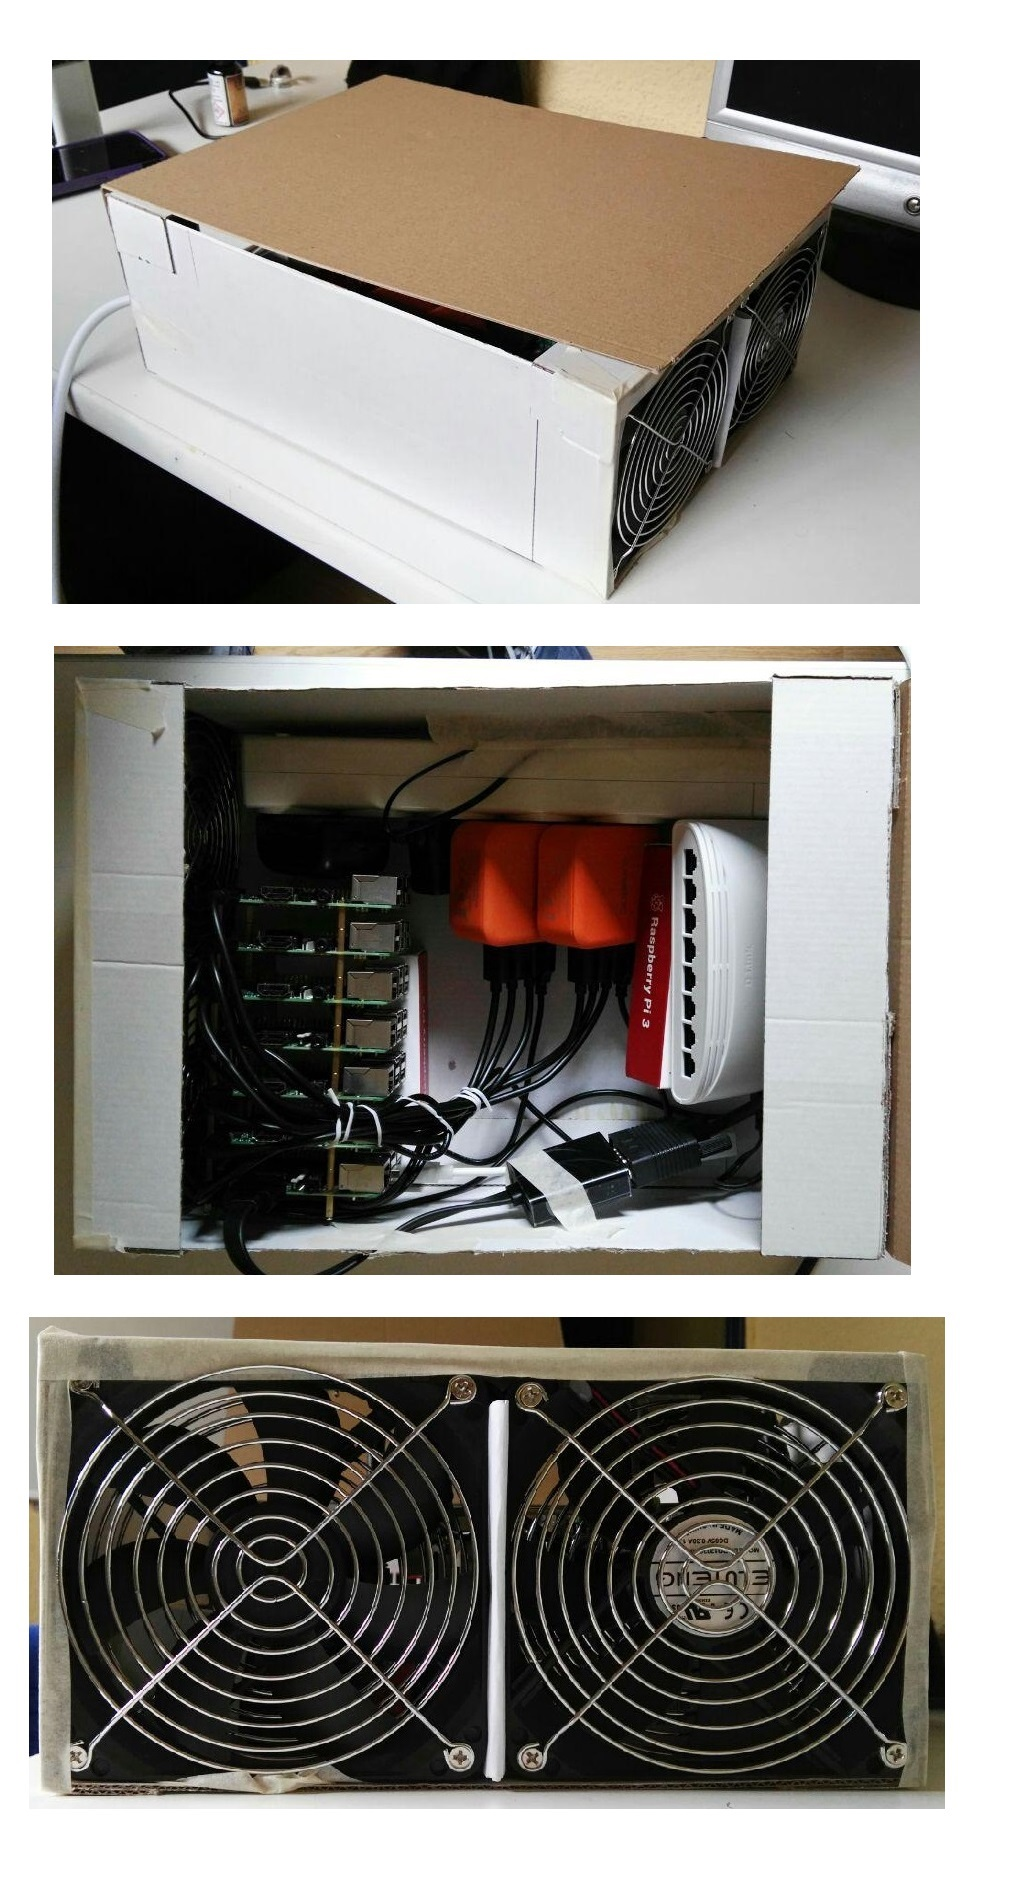
\includegraphics[width=60mm]{Modelos/M1Res.jpg}
   	\caption[Resultado Modelo 1]{Resultado Modelo 1}
   \label{figure4.2}
\end{figure}

Las figura \ref{figure4.2} muestra el resultado del diseño descrito en el apartado anterior, se puede observar la distribución de los componentes dentro del contenedor y el cierre del que dispone.

\section{Modelo 2}
\label{makereference4.4}
\paragraph{}

Para resolver los problemas de accesibilidad al rack este modelo dispone de una apertura lateral que expone las tarjetas \textbf{SD} de cada Raspberry, con lo que no es necesario abrir el contenedor para extraer cada tarjeta.
Además el contenedor está dividido en dos piezas, una que se acopla sobre la otra para formar un cubo, esto facilita la apertura y acceso al mismo.

\begin{figure}[H]
	\centering
  	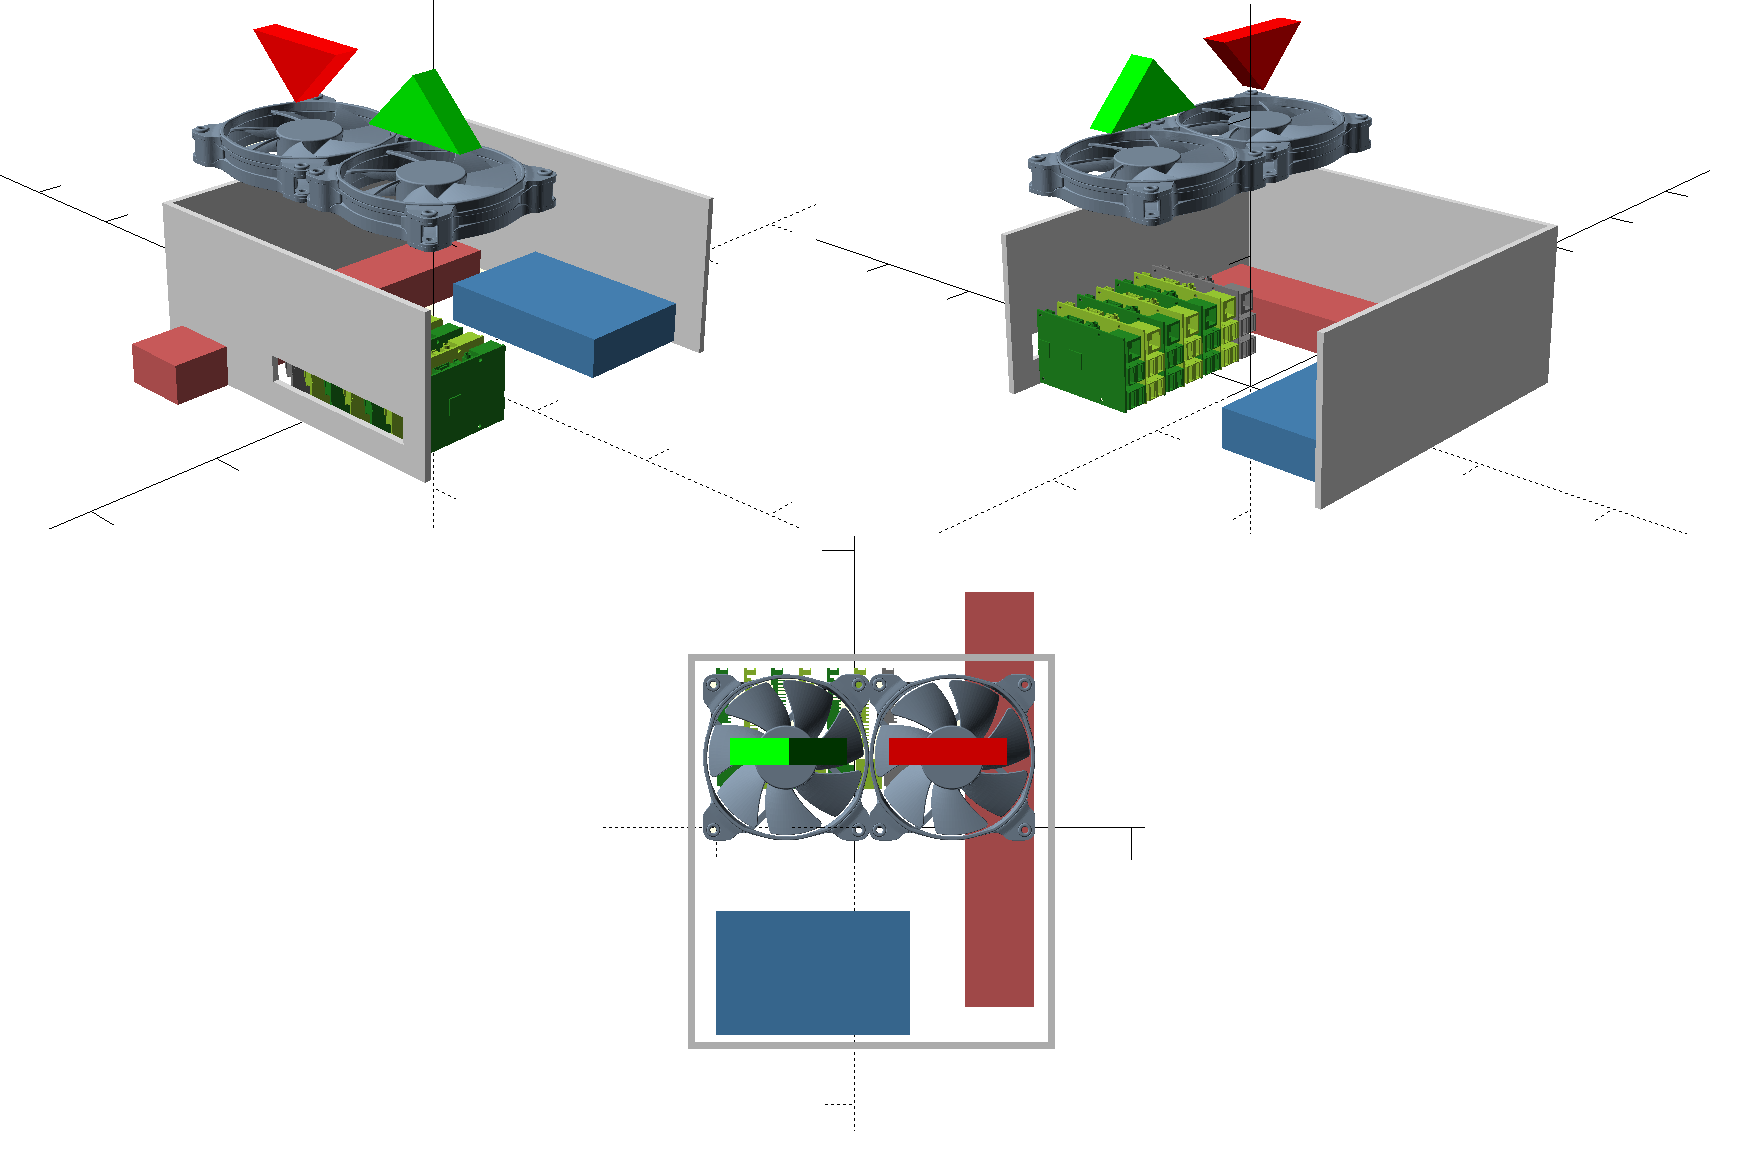
\includegraphics[width=120mm]{Modelos/M2X.png}
   	\caption[Modelo 2 3D]{Modelo 2 3D}
   \label{figure4.3}
\end{figure}

Como se muestra en la figura \ref{figure4.3} la ventilación se realiza desde la parte superior, creando, como en el caso anterior, una corriente de aire debida al emplazamiento de cada ventilador. Se puede observar, en la vista frontal, la apertura centrada sobre el rack de Raspberrys.
Este modelo es más compacto que el anterior, parte de la base de enchufes queda en el exterior. Sin embargo, existe un mayor espacio entre los ventiladores y el rack.
La disposición de los cables de alimentación del rack es mejor que la del modelo 1, junto con el acceso lateral, prácticamente no es necesario manipular ninguno de los componentes.

\subsection{Resultado}
\paragraph{}

Este modelo tiene un tamaño de 122x123x35 cm, en la figura \ref{figure4.4} se puede observar el sistema de acople en dos piezas que abren el contenedor. Como se ha comentado anteriormente, parte de la base de enchufes queda en el exterior, esto supone una mejora ya que permite el encendido y apagado del clúster sin que sea necesario abrir todo el contenedor para ello. 

\begin{figure}[H]
	\centering
  	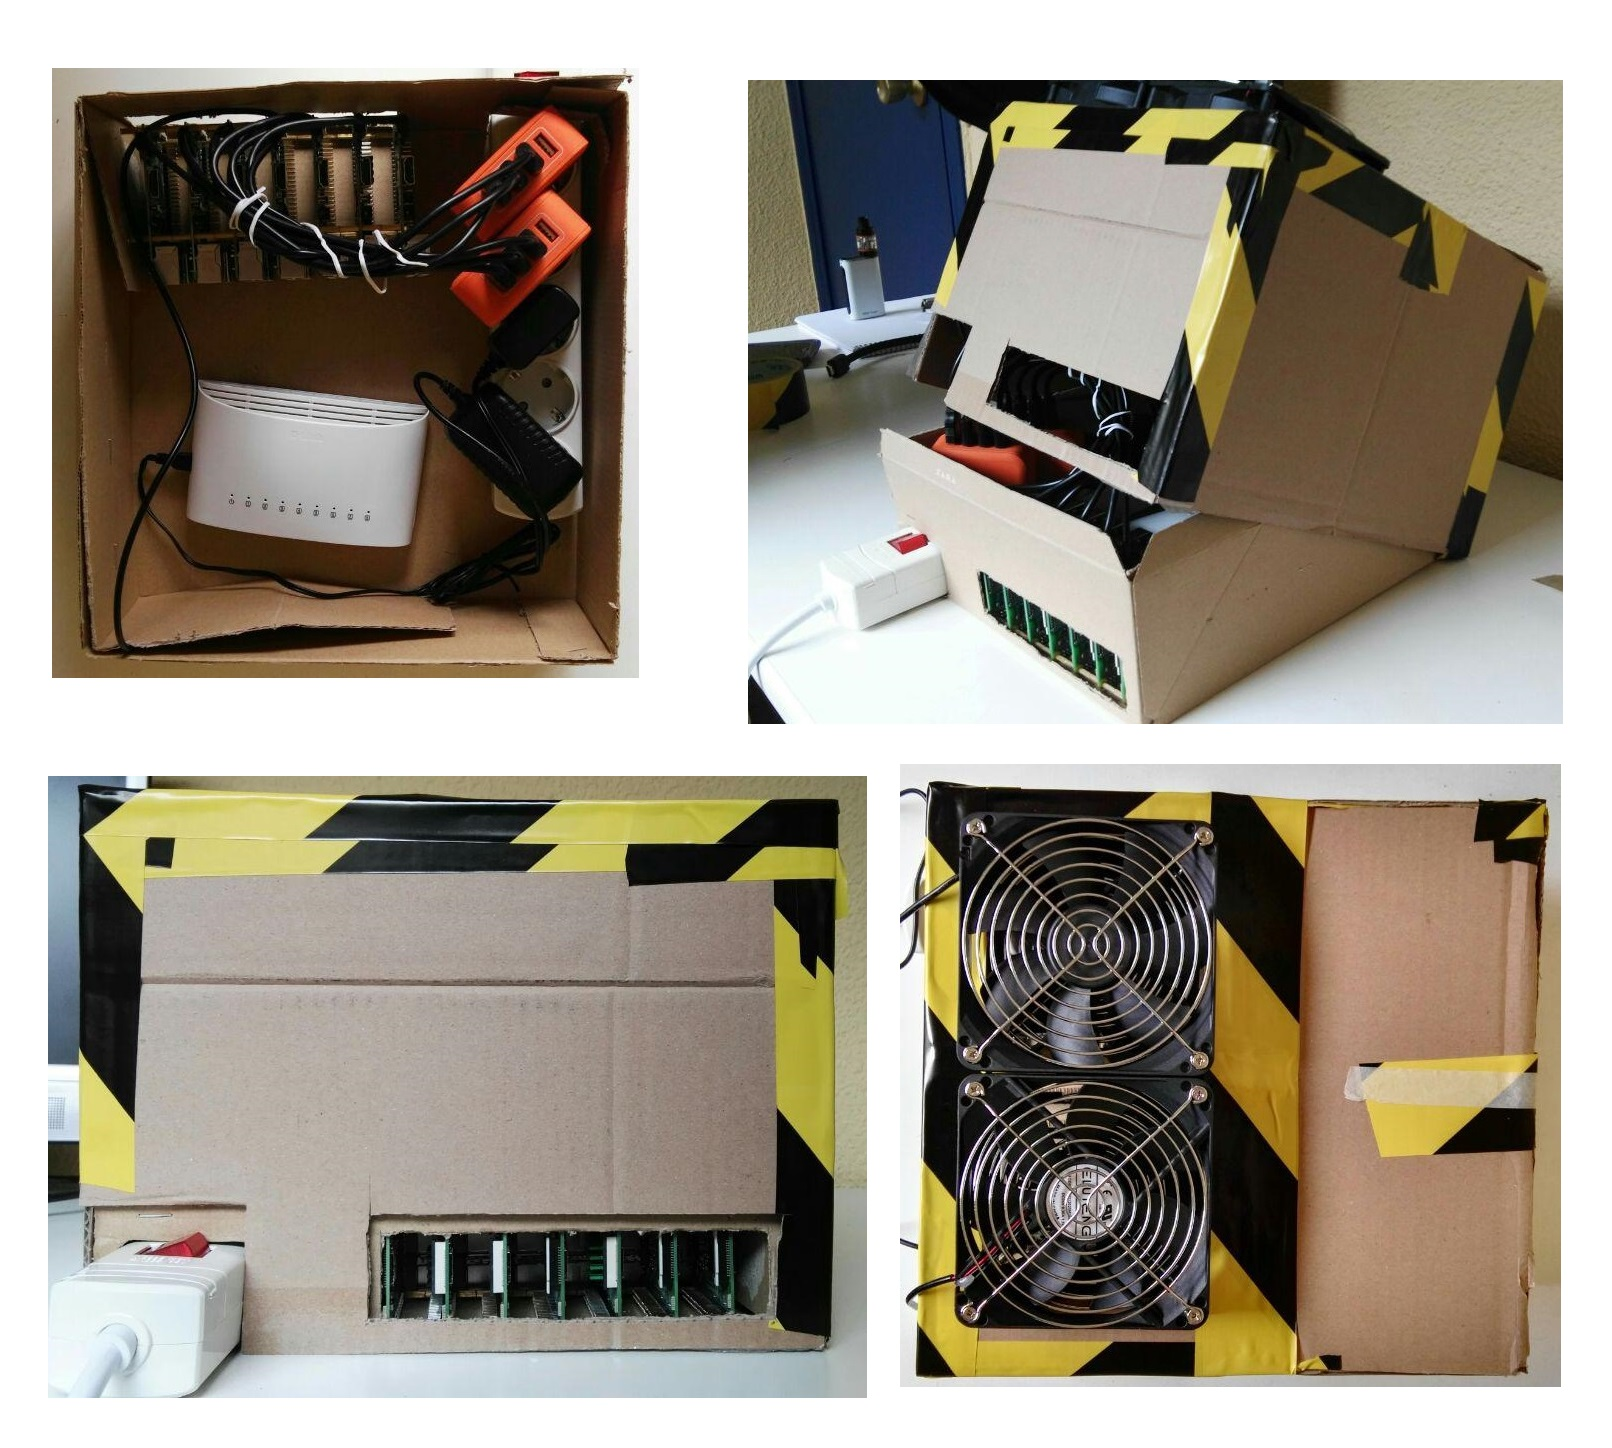
\includegraphics[width=100mm]{Modelos/M2Res.jpg}
   	\caption[Resultado Modelo 2]{Resultado Modelo 2}
   \label{figure4.4}
\end{figure}

Como resultado de todas estas mejoras tenemos un modelo que es mucho mas manejable que el anterior, de tamaño más reducido y con mejoras estructurales que facilitan la manipulación.

\section{Modelo 2b}
\label{makereference4.5}
\paragraph{}

El modelo 2b presenta unas modificaciones estructurales internas, tras hacer un estudio previo sobre corrientes de aire decidimos realizar algunas modificaciones sobre éste para conseguir mejorar la eficiencia del flujo de aire dentro del contenedor.

\begin{figure}[H]
	\centering
  	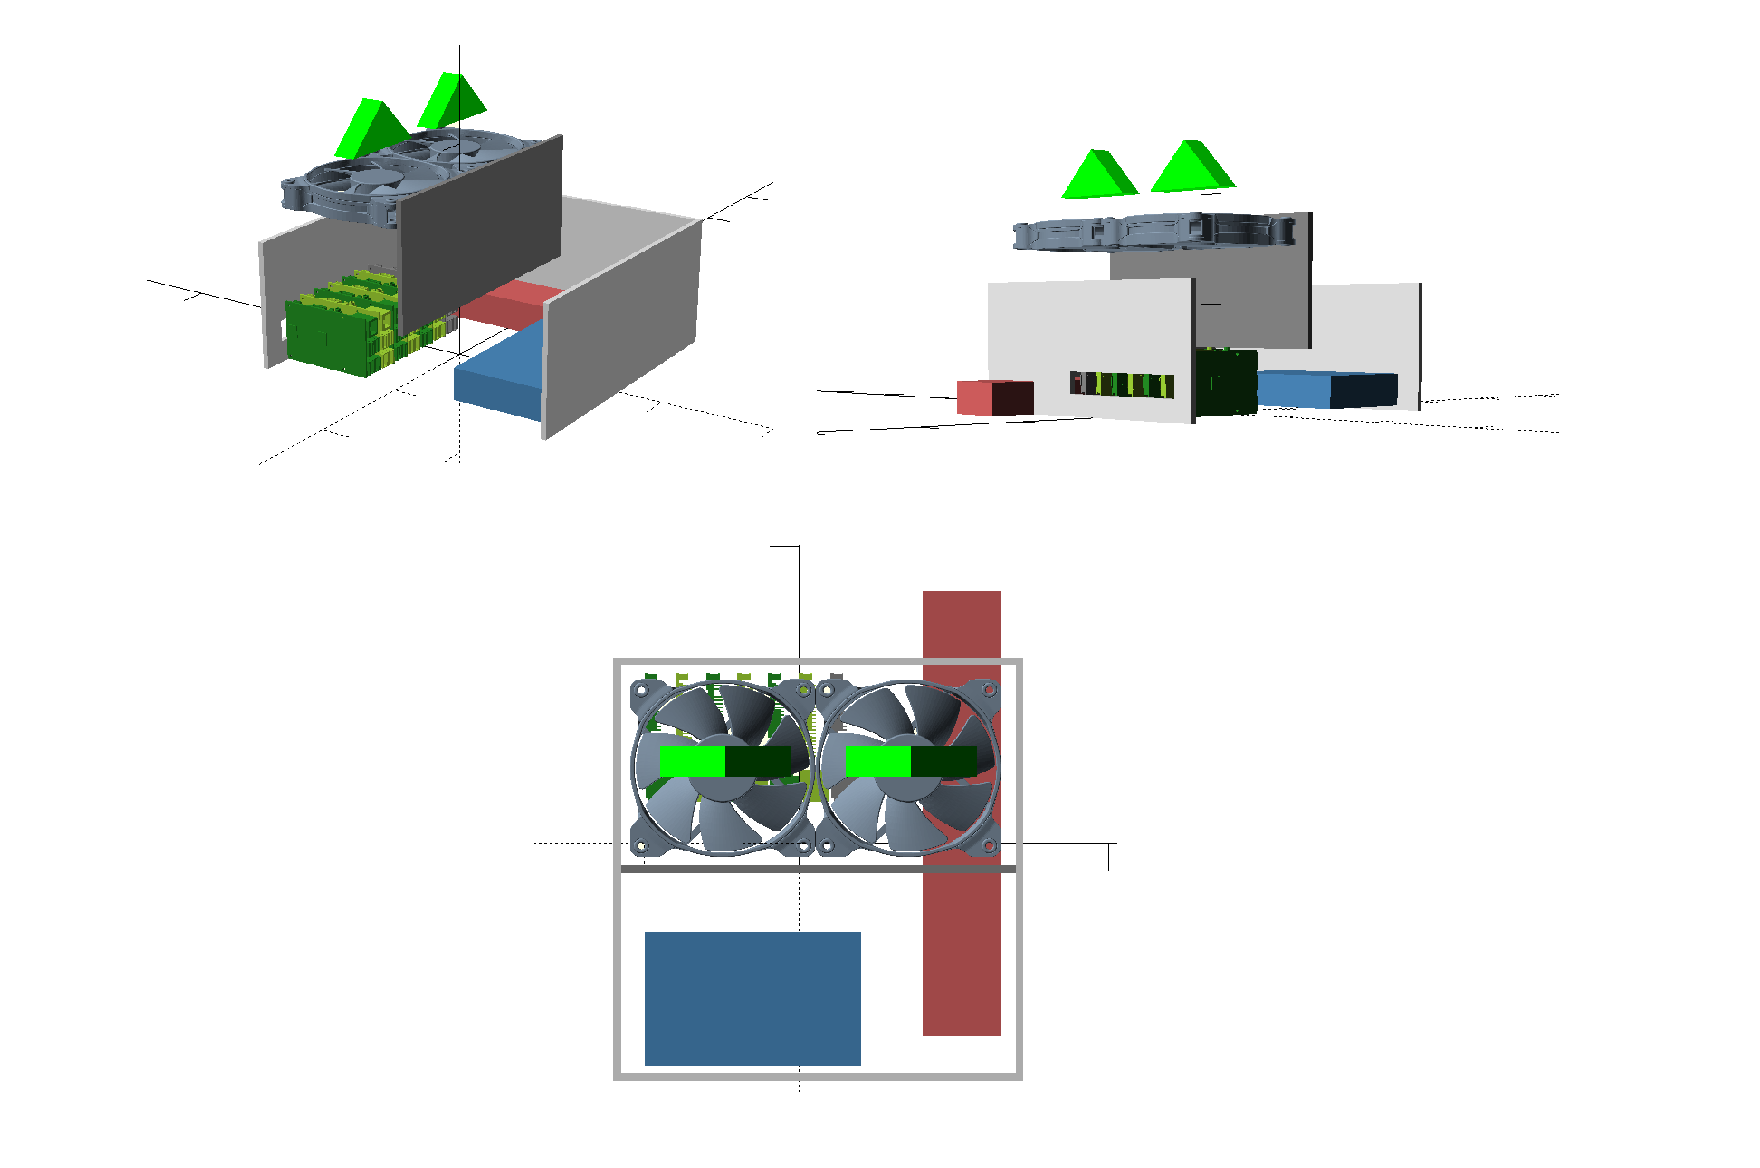
\includegraphics[width=120mm]{Modelos/M2bX.png}
   	\caption[Modelo 2b 3D]{Modelo 2b 3D}
   \label{figure4.5}
\end{figure}

Para esto, se incluye una nueva pared interior, distribuyendo el contenedor en \textit{dos cámaras}, una que contiene el rack de Raspberrys y otra con el switch. La corriente de aire se concentra en la primera cámara, con esto generamos un flujo que entra en el contenedor a través de la entrada lateral, en la que están expuestas las Raspberrys, pasando por cada uno de los procesadores y saliendo por la parte superior en la que ambos ventiladores expulsan el aire.

La figura \ref{figure4.5}, similar a la del modelo 2, muestra la separación en cámaras y distribución de los ventiladores.
Como se puede comprobar en el capítulo \ref{ch:capitulo5.tex} esta modificación ofrece unos resultados completamente distintos en cuanto a las temperaturas del contenedor.


\section{Modelo 3}
\label{makereference4.6}
\paragraph{}

Hemos diseñado el modelo 3 utilizando la arquitectura de \textit{túnel de viento}, éste consiste en suministrar una corriente de aire de entrada sobre las partes que más tienden a calentarse, en este caso, el rack de Raspberrys, aplicando una corriente de succión con un ventilador de salida, creando un flujo de aire horizontal. 
 
\subsection{Modelado 3D}
\paragraph{}

\begin{figure}[H]
	\centering
  	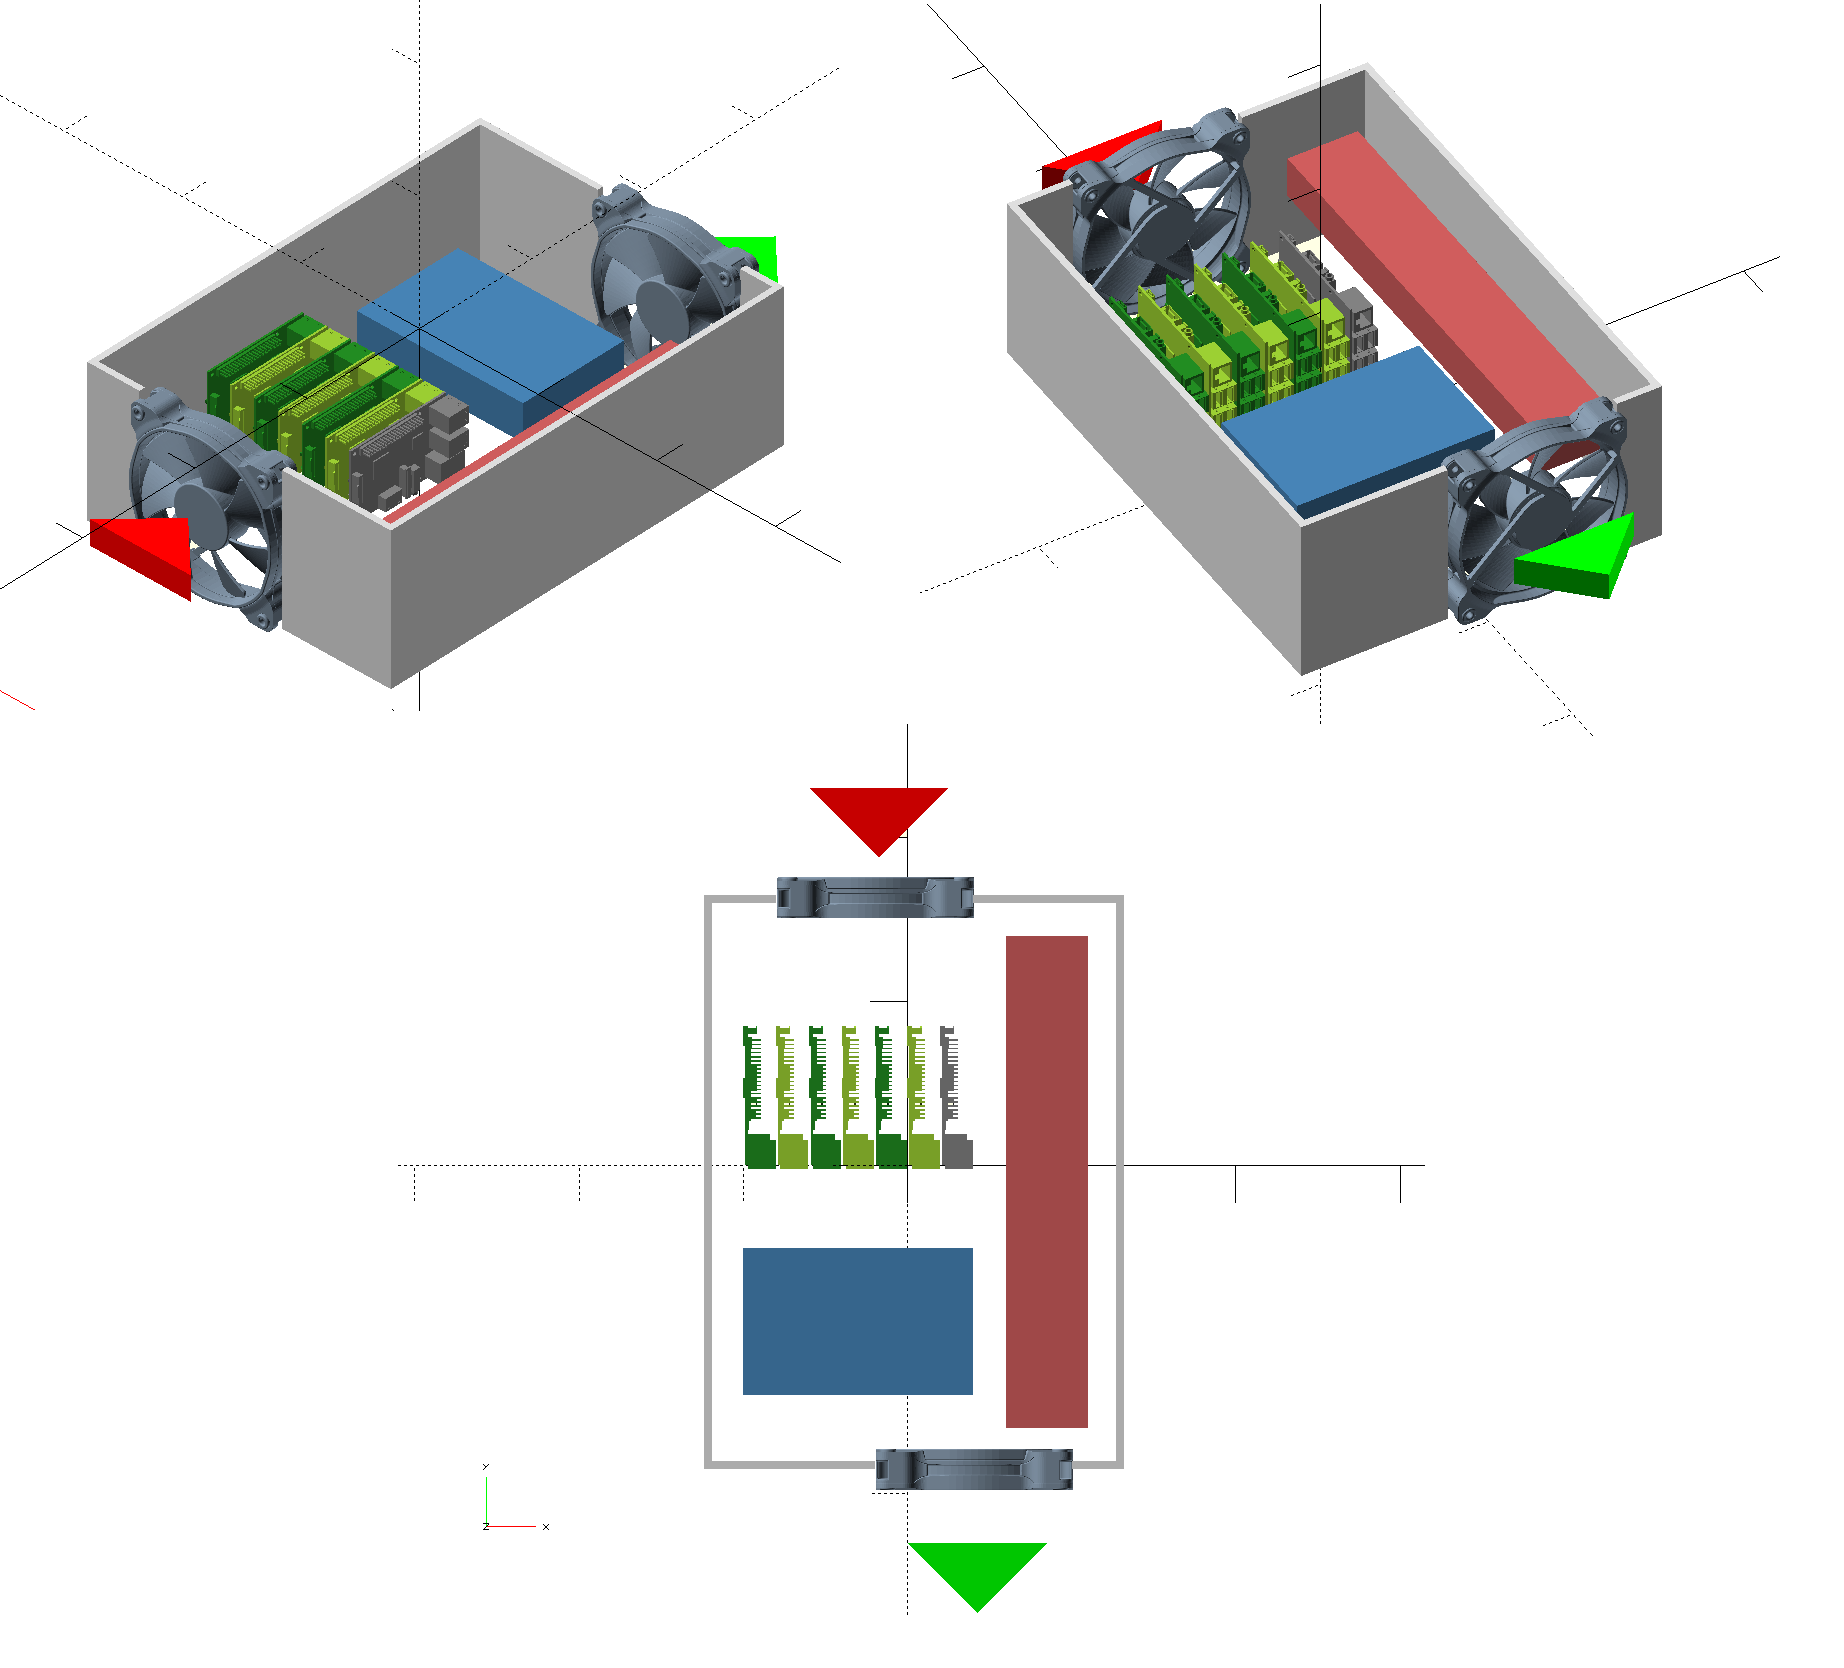
\includegraphics[width=100mm]{Modelos/M3X.png}
   	\caption[Modelo Modelo 3 3D]{Modelo 3 3D}
   \label{figure4.6}
\end{figure}

Debido a las altas temperaturas presentadas por el modelo 1 decidimos aplicar una corriente de aire directa sobre las Raspberrys y sacarla del sistema para evitar bucles de aire calientes a través del segundo ventilador que está situado al lado del switch como se muestra en la figura \ref{figure4.6} 

Tras una serie de pruebas y mediciones de temperatura con la disposición de los ventiladores, entrada-salida, entrada-entrada y salida-salida, llegamos a la conclusión que la más eficiente era la primera de ellas.

\subsection{Resultado}
\paragraph{}

Tras el desarrollo de los modelos anteriores, hemos creado un híbrido entre el modelo 1 y 2B, del primero aprovechamos su base y el ventilador del que ya disponíamos, del segundo, hemos decidido que en vez de aplicar la corriente de succión en la parte de arriba, le otorgaremos un flujo de aire que recorre todo el contenedor a través del túnel de viento ya mencionado. Mientras los anteriores modelos se centraban en las Raspberrys, este proporciona una corriente tanto al Switch como al rack. 

\begin{figure}[H]
	\centering
  	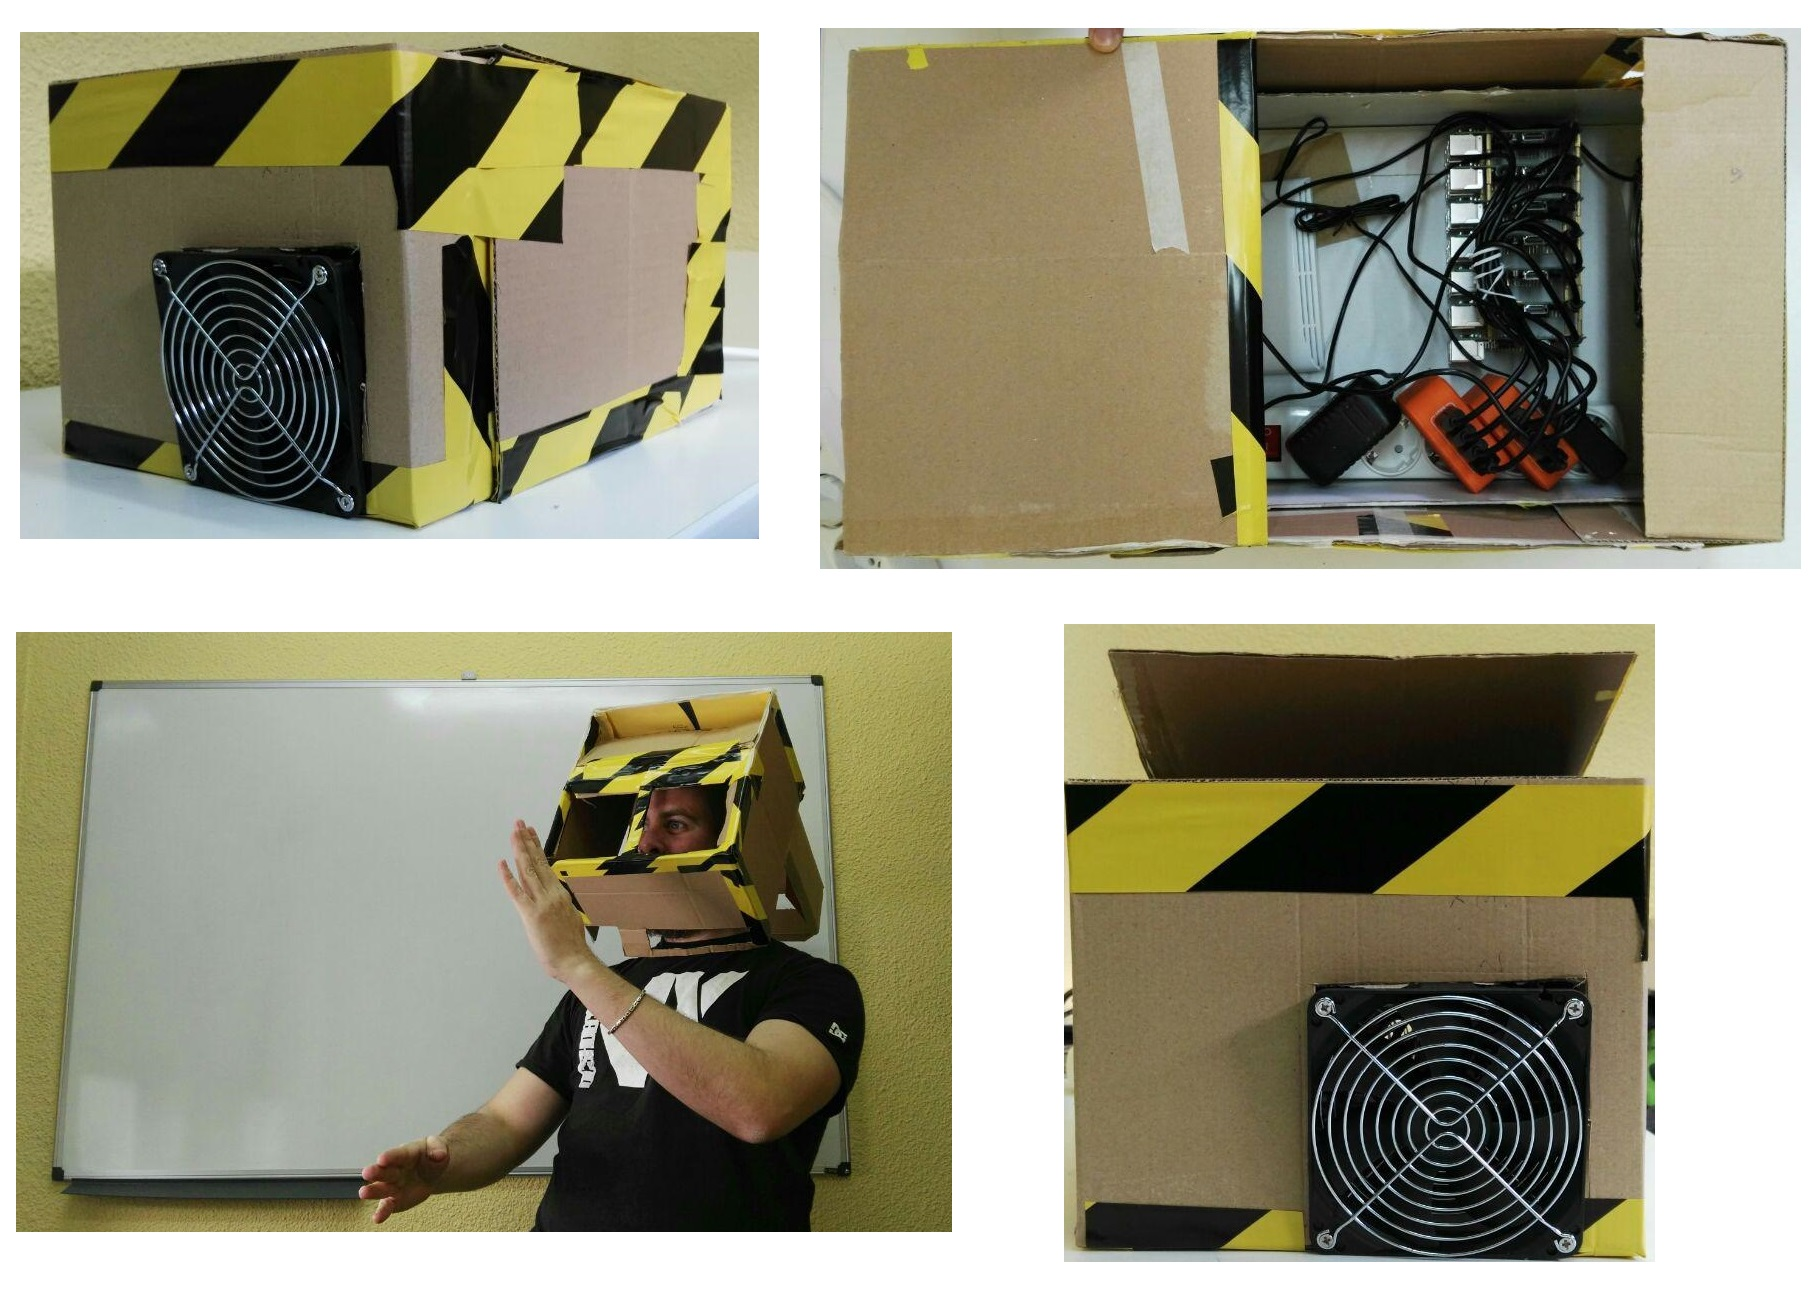
\includegraphics[width=100mm]{Modelos/M3Res.jpg}
   	\caption[Resultado Modelo 3]{Resultado Modelo 3}
   \label{figure4.7}
\end{figure}

El T-800 de la figura \ref{figure4.7} no está incluido en el pack, presentó demasiadas complicaciones a nivel de diseño y entraba continuamente en conflicto debido a las tres leyes de la robótica.

\newpage
\chapter{Tests de Diseño}
\label{ch:capitulo5.tex}

\begin{FraseCelebre}
	\begin{Frase}
		Tendrá todo el dinero del mundo, pero hay algo que nunca podrá comprar… un dinosaurio.
	\end{Frase}
	\begin{Fuente}
	Homer J. Simpson
	\end{Fuente}
\end{FraseCelebre}

El objetivo de este capítulo es el de mostrar el resultado de las pruebas de temperaturas realizadas en los diferentes modelos diseñados en el capítulo \ref{ch:capitulo4.tex}. 

\section{Experimental Settings}
\label{makereference5.2}
\paragraph{}

Se ha sometido a estos a un total de tres pruebas, todas ellas con las mismas características para cada modelo, variando en el número de nodos que hay trabajando de forma simultánea en cada caso. De esta manera, según los resultados obtenidos y las características de diseño generadas en el capítulo \ref{ch:capitulo4.tex} determinamos qué modelo es el más idóneo para la elección final.

Además de las pruebas generales, se han realizado una serie de pruebas específicas para cada modelo, el objetivo de estas, ha sido el de determinar la mejor configuración en cuanto a la disposición de los ventiladores dentro del contenedor. En este capítulo, únicamente se muestran las pruebas realizadas a los modelos finales.

Para el desarrollo de cada prueba se ha generado un script que obtiene información de la temperatura del procesador ofrecida directamente por el sistema operativo. El siguiente cuadro muestra el contenido del script:

\begin{lstlisting}[language=c++,frame=single,numbers=none]
	#!/bin/bash
  while test 0 -eq 0 
  do
    sleep $1
    temp=$(/opt/vc/bin/vcgencmd measure_temp | cut -c 6-9)
    time=$(date +"%x" ) #dd/mm/yyyy
    echo "$temp"  
  done
  exit 0
\end{lstlisting}

\section{Prueba 1}
\label{makereference5.3}

\subsection{Escenario}
\paragraph{}

En esta prueba únicamente hay una Raspberry Pi trabajando con cuatro cores, el tiempo total de cada prueba es de tres horas, el periodo de muestreo es de diez segundos y en las gráficas se muestra el tiempo total expresado en segundos. La temperatura ambiente oscila entre los catorce y dieciocho grados. Ninguna de las raspberrys utilizadas dispone de un disipador instalado sobre el procesador.

\subsection{Resultados}

\begin{figure}[H]
	\centering
  	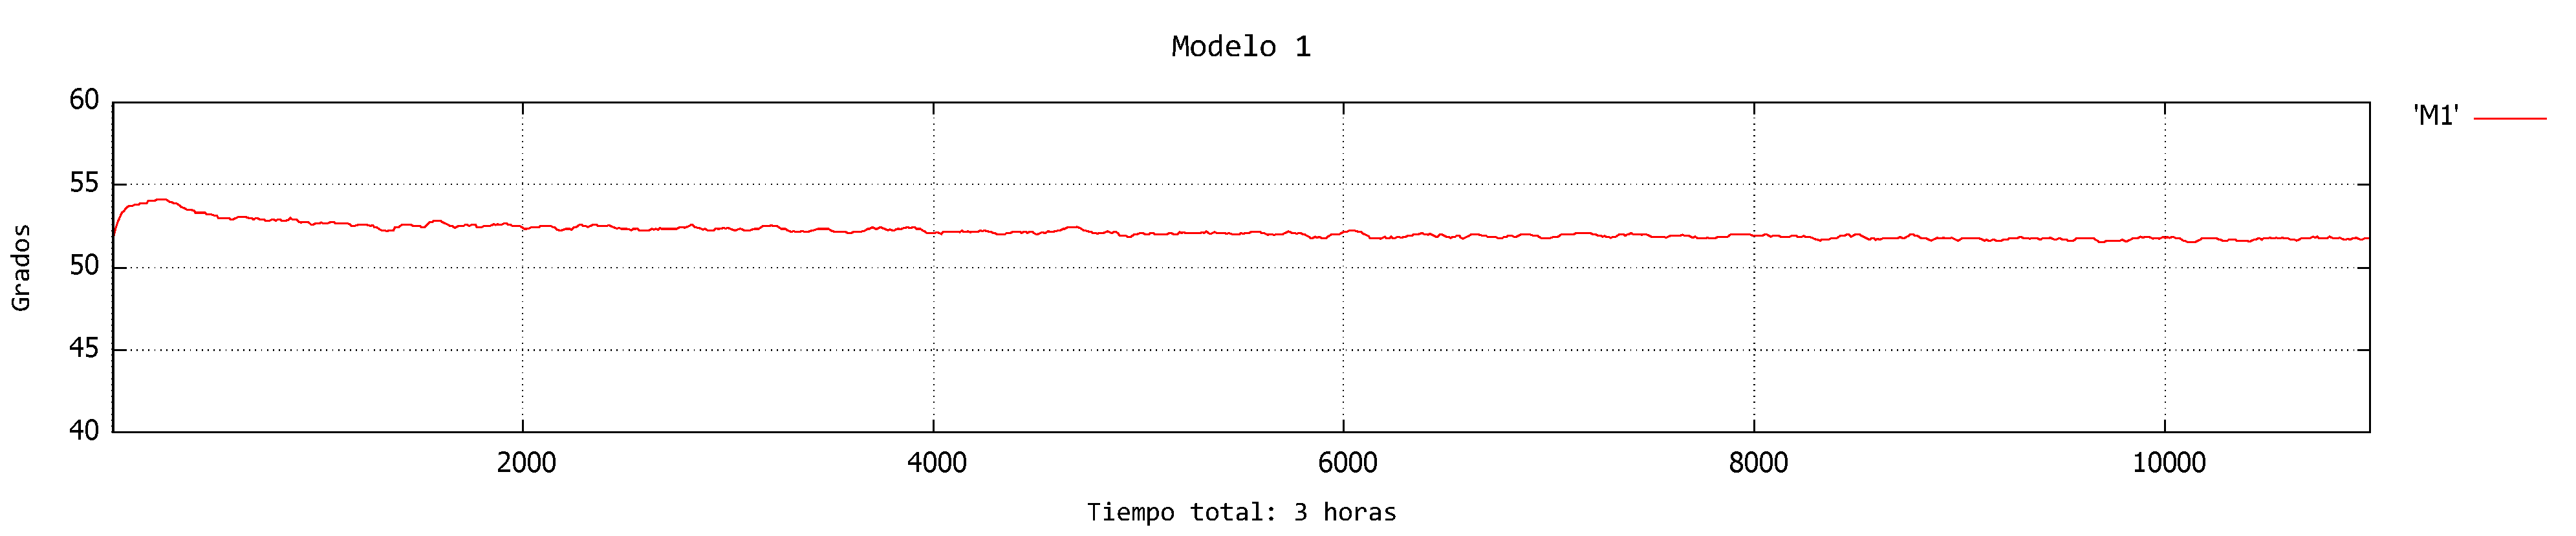
\includegraphics[width=160mm]{Test/Pr1_modelo1.pdf}
   	\caption[Prueba 1, Modelo 1]{Modelo 1}
   \label{figure5.1}
\end{figure}

\begin{figure}[H]
	\centering
  	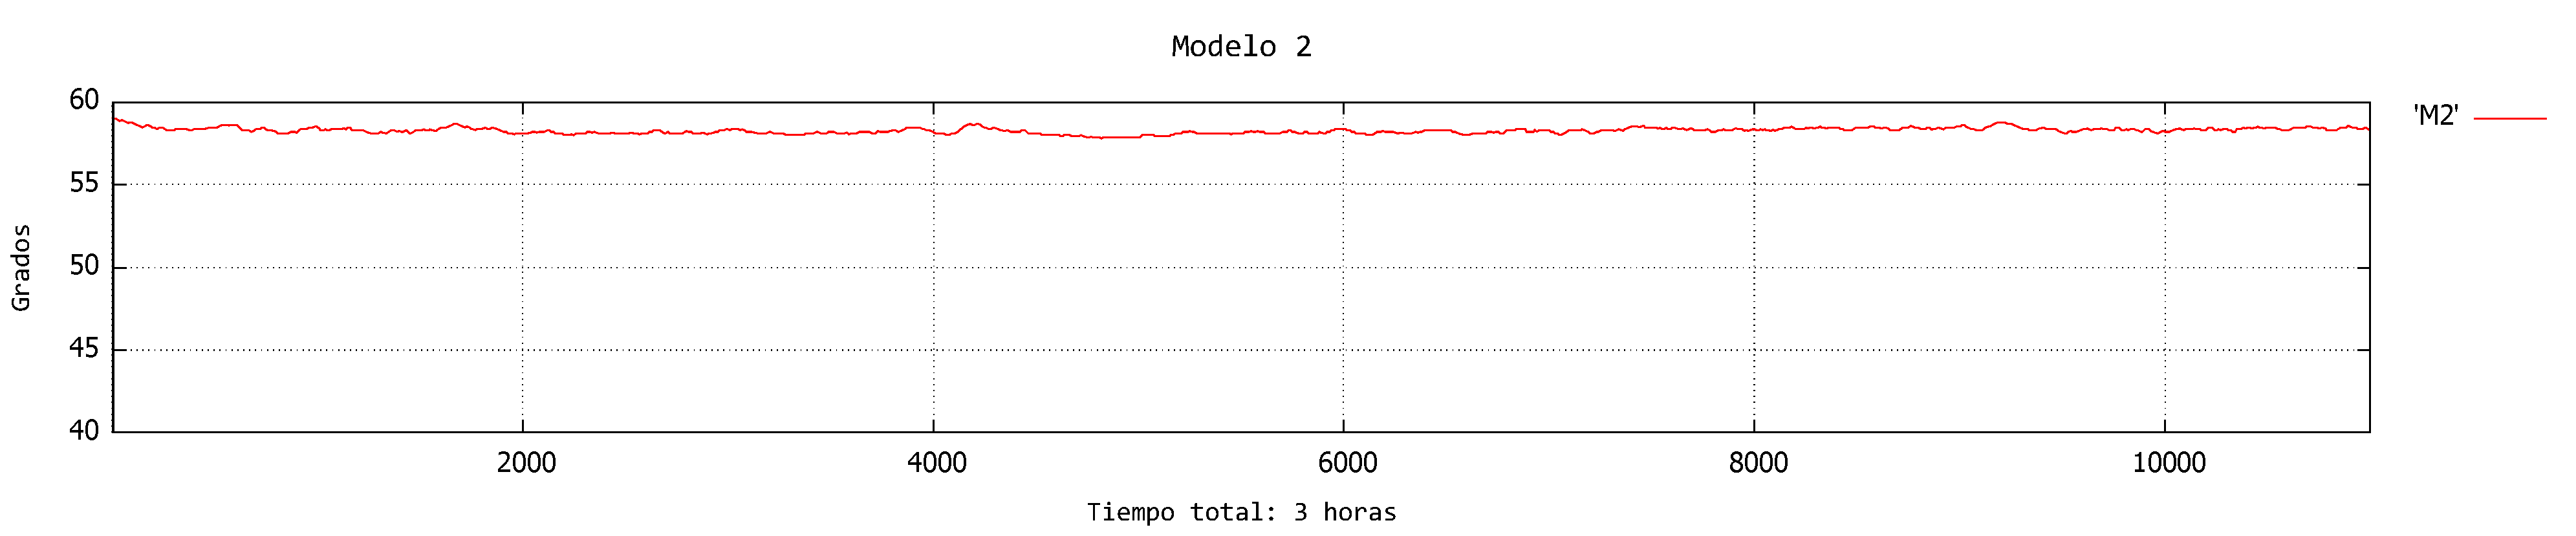
\includegraphics[width=160mm]{Test/Pr1_modelo2.pdf}
   	\caption[Prueba 1, Modelo 2]{Modelo 2}
   \label{figure5.2}
\end{figure}

\begin{figure}[H]
	\centering
  	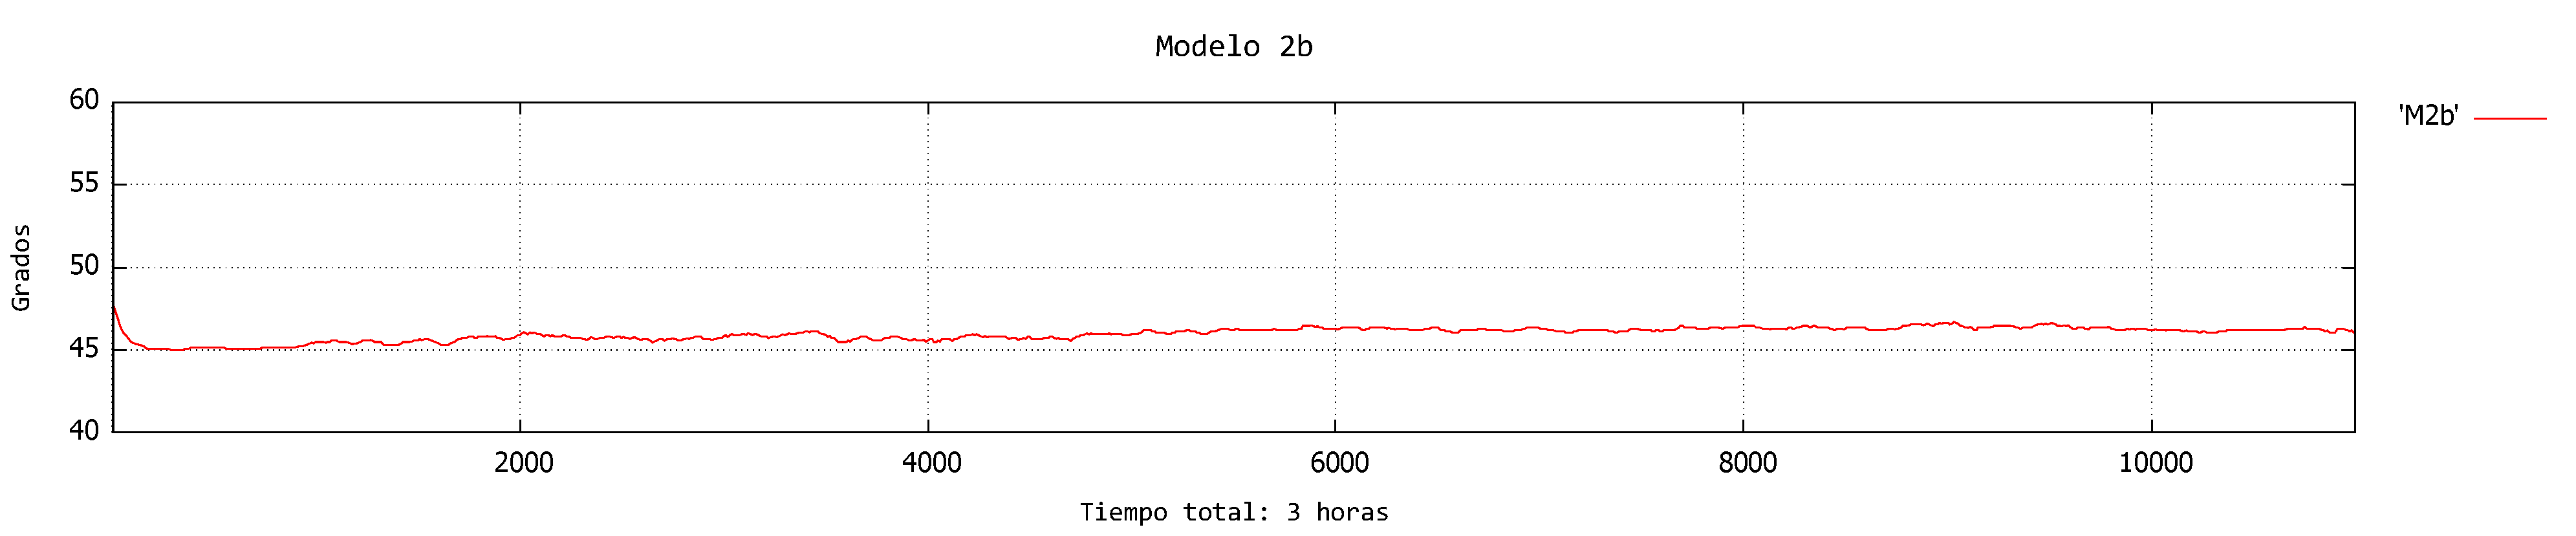
\includegraphics[width=160mm]{Test/Pr1_modelo2b.pdf}
   	\caption[Prueba 1, Modelo 2b]{Modelo 2b}
   \label{figure5.3}
\end{figure}

\begin{figure}[H]
	\centering
  	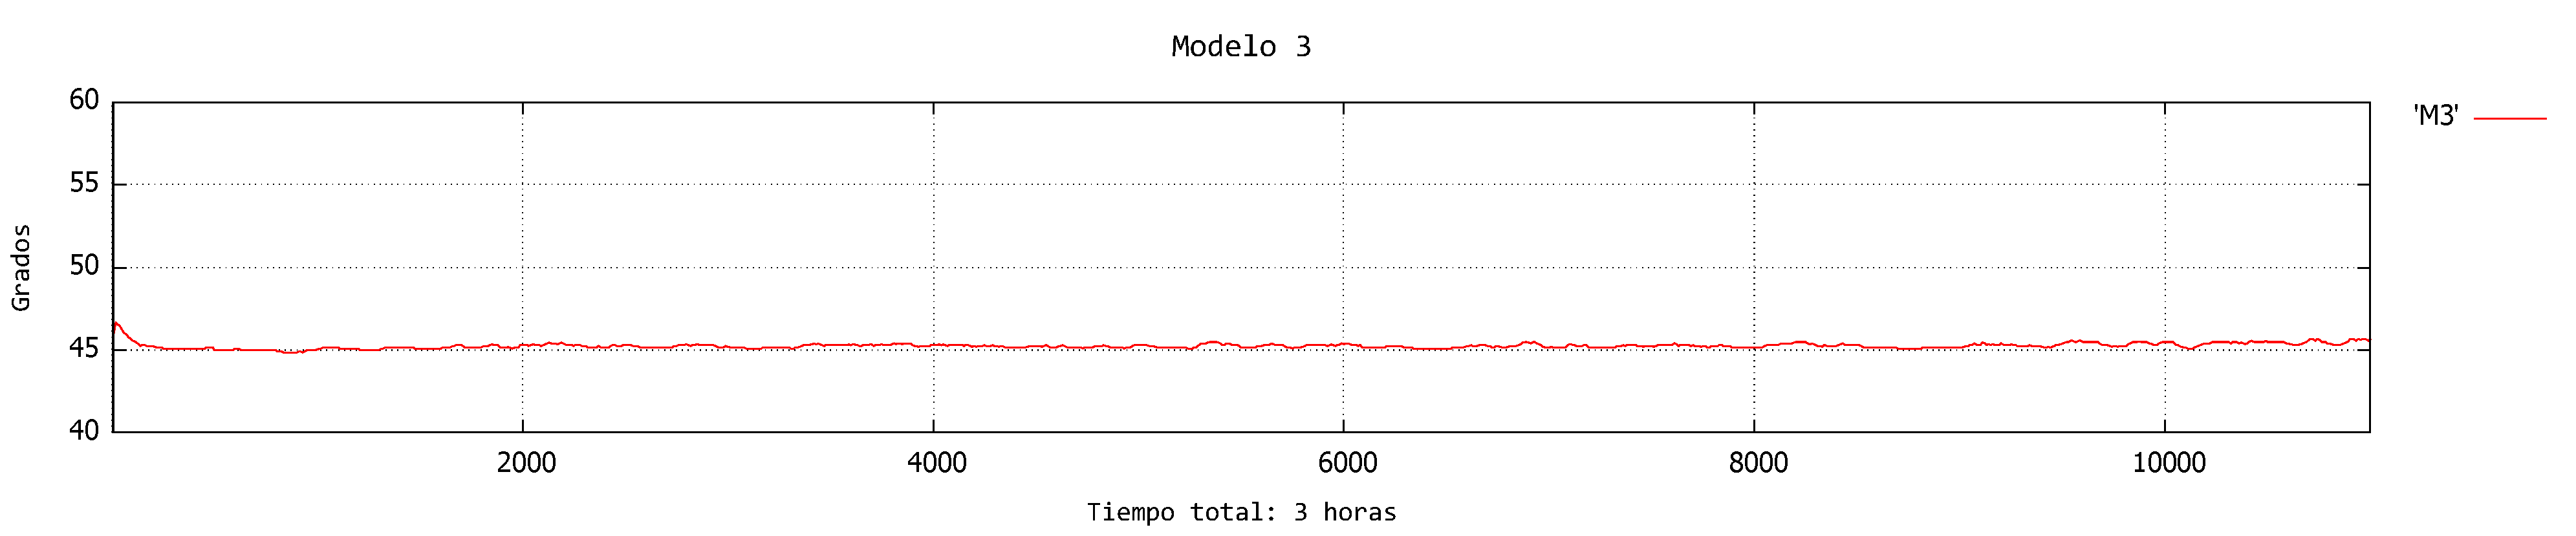
\includegraphics[width=160mm]{Test/Pr1_modelo3.pdf}
   	\caption[Prueba 1, Modelo 3]{Modelo 3}
   \label{figure5.4}
\end{figure}

\subsection{Conclusiones}
\paragraph{}

Se puede comprobar que tanto el modelo 2b como el modelo 3 son los que obtienen unos mejores resultados, en todo caso, en todos ellos, el sistema se mantiene estable durante toda la prueba, con muy poca variación entre sus temperaturas máxima y mínima. El modelo 2 registra unos valores cercanos a los sesenta grados, con lo que es sin duda el peor de los tres.

\section{Prueba 2}
\label{makereference5.4}
\subsection{Escenario}
\paragraph{}

En esta prueba hay tres Raspberrys trabajando de forma simultánea, cada una de ellas mantiene sus cuatro cores trabajando a máximo rendimiento, el tiempo total de las pruebas es nuevamente de tres horas, igual que en la prueba anterior el periodo de muestreo es de diez segundos y en cada gráfica muestra el tiempo total expresado en segundos. La temperatura ambiente, en este caso, oscila entre los quince y dieciocho grados. Una de las Raspberrys dispone de un disipador de calor, en las gráficas, esta se identifica con la letra D al lado de su nombre.

\subsection{Resultados}
\paragraph{}

\begin{figure}[H]
	\centering
  	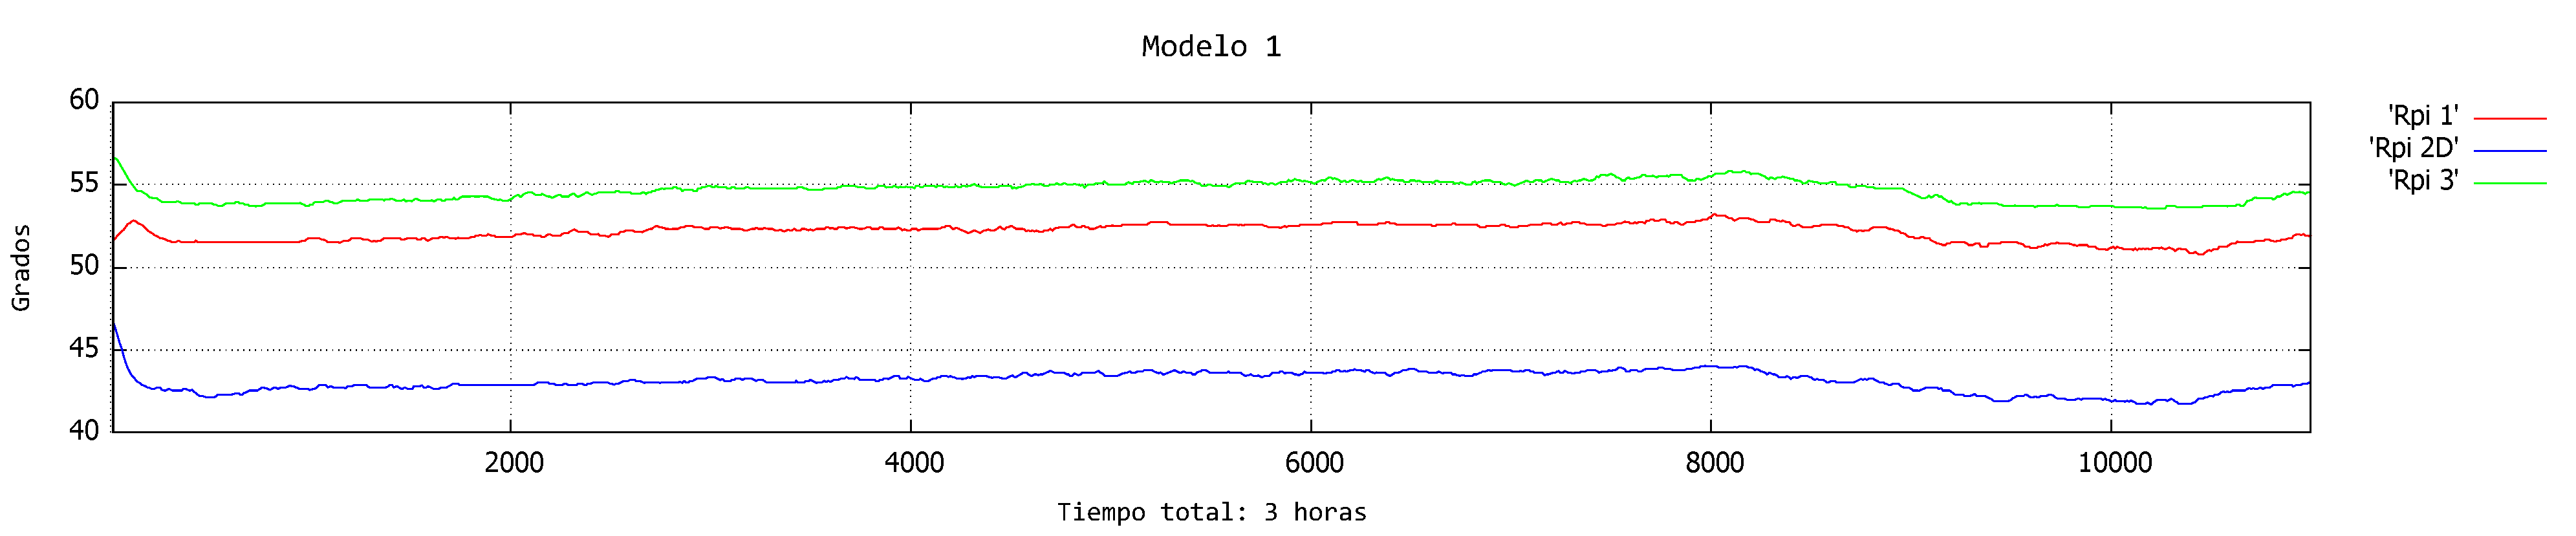
\includegraphics[width=160mm]{Test/pr2_modelo1.pdf}
   	\caption[Prueba 2, Modelo 1]{Modelo 1}
   \label{figure5.5}
\end{figure}

\begin{figure}[H]
	\centering
  	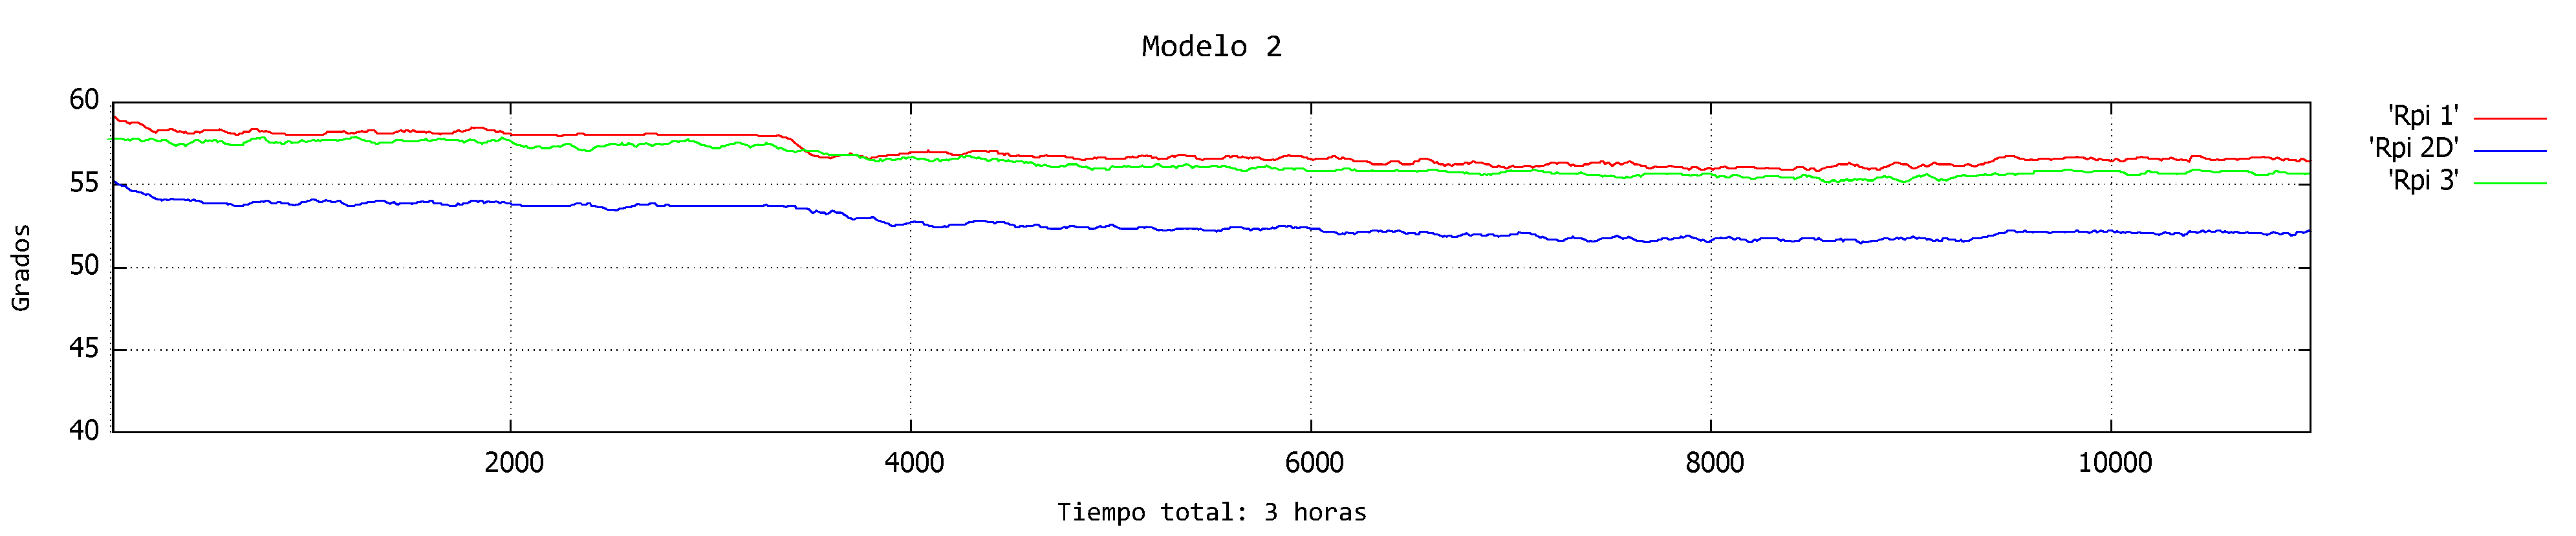
\includegraphics[width=160mm]{Test/pr2_modelo2.pdf}
   	\caption[Prueba 2, Modelo 2]{Modelo 2}
   \label{figure5.6}
\end{figure}

\begin{figure}[H]
	\centering
  	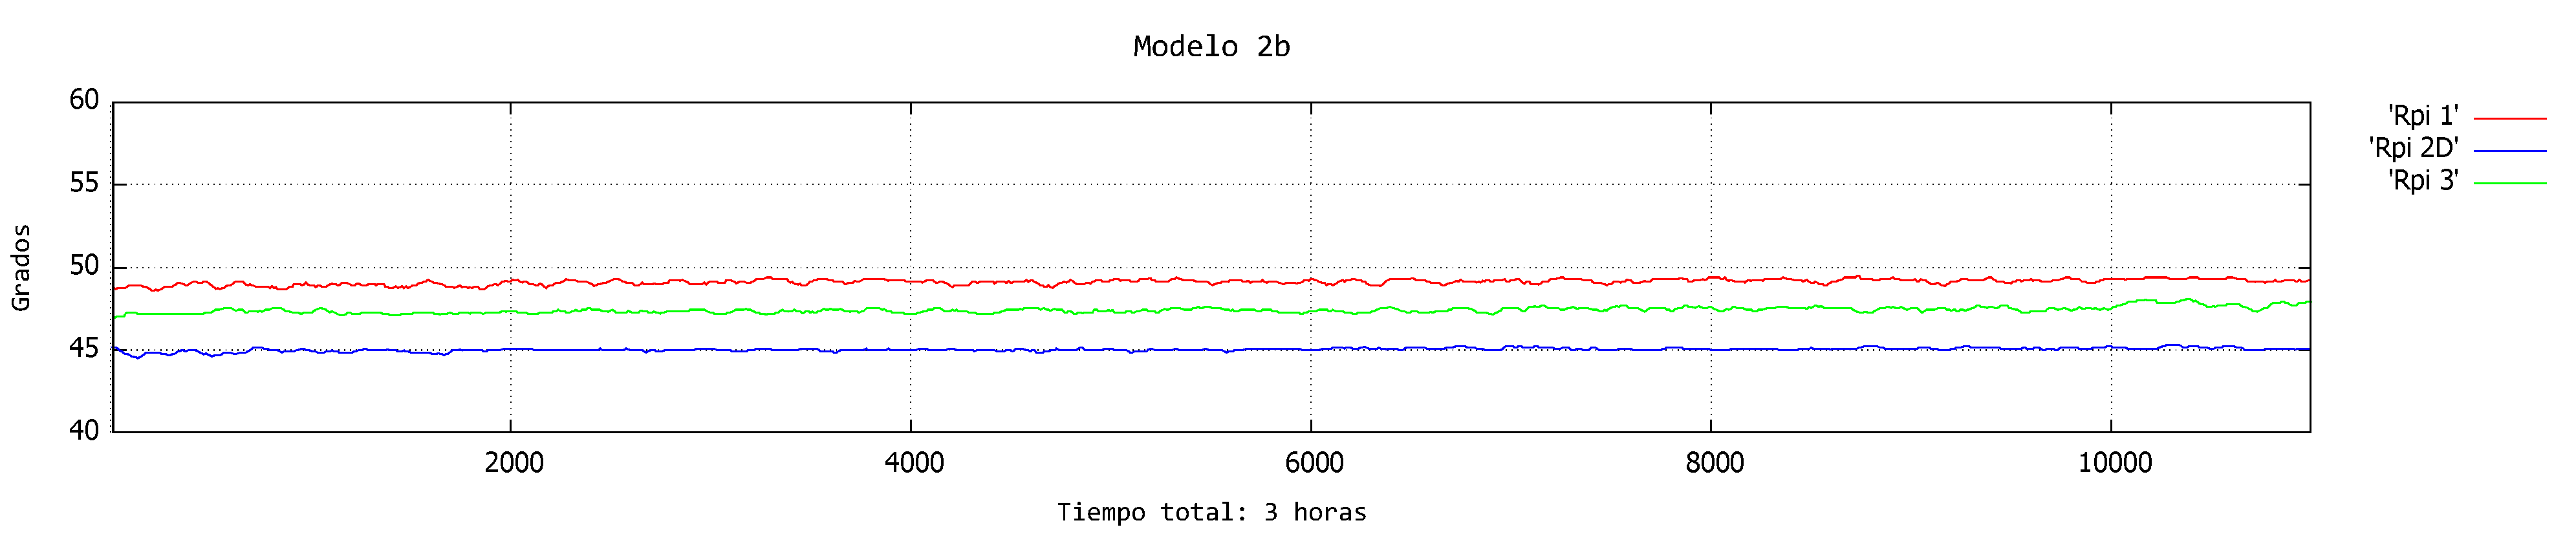
\includegraphics[width=160mm]{Test/pr2_modelo2b.pdf}
   	\caption[Prueba 2, Modelo 2b]{Modelo 2b}
   \label{figure5.7}
\end{figure}

\begin{figure}[H]
	\centering
  	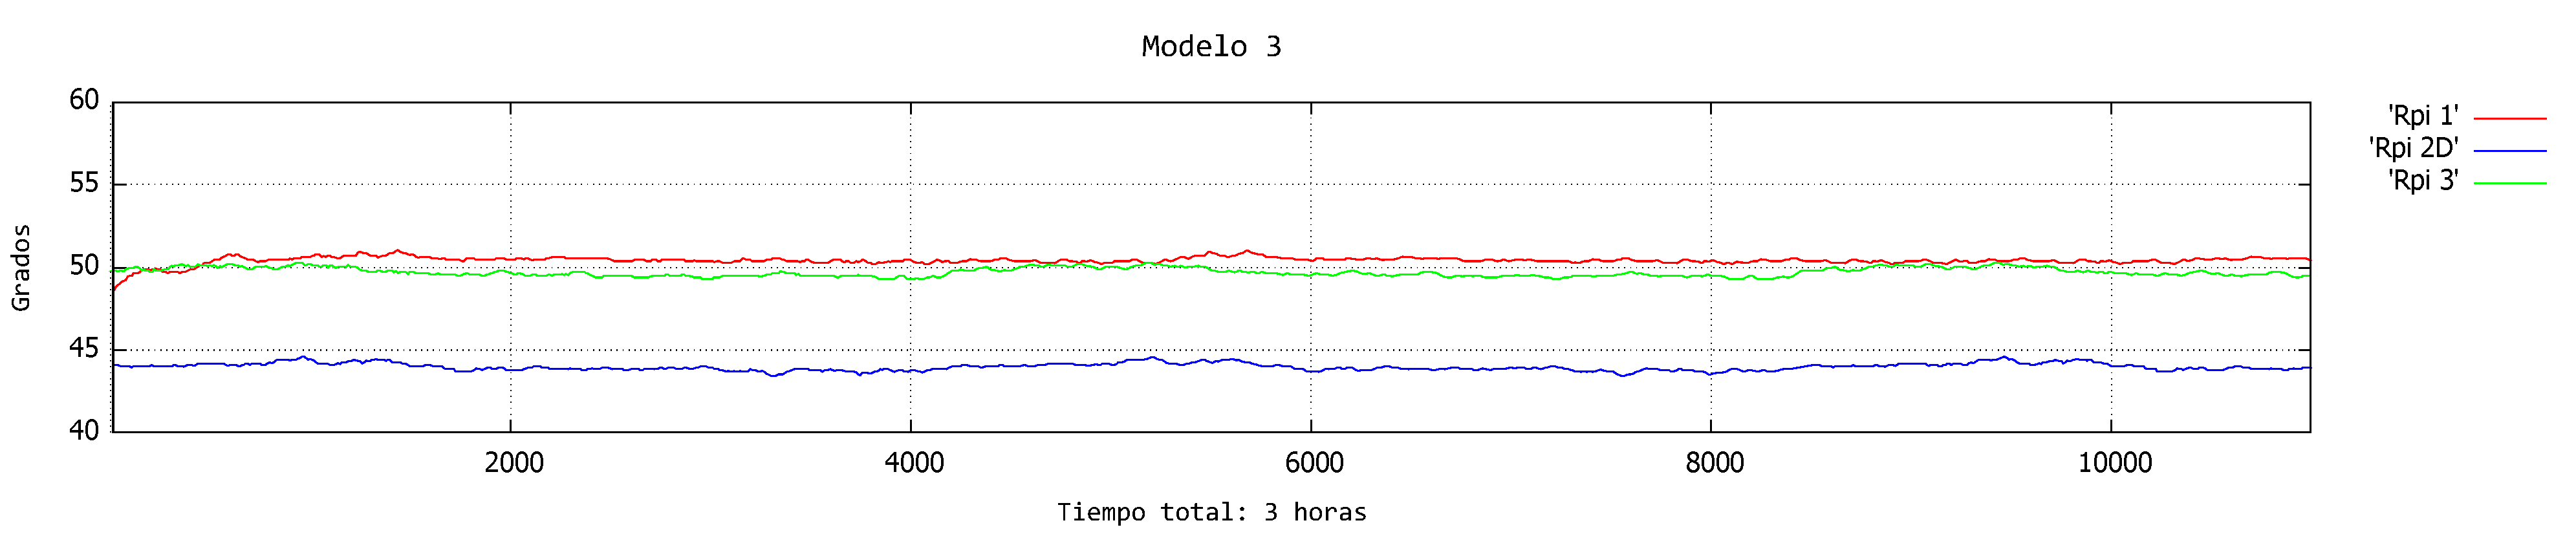
\includegraphics[width=160mm]{Test/pr2_modelo3.pdf}
   	\caption[Prueba 2, Modelo 3]{Modelo 3}
   \label{figure5.8}
\end{figure}

\subsection{Conclusiones}
\paragraph{}

Hemos comprobado que una buena corriente de aire hace que aquellos nodos que disponen de un disipador de calor instalado presenten unas temperaturas notablemente inferiores al resto. Sin embargo, como pasa en el modelo 2, figura \ref{figure5.6}, si la corriente no es eficiente, dicha mejora se ve severamente afectada.

De nuevo, los modelos 2b y 3, ofrecen unos resultados mejores, además se mantienen más estables durante toda la prueba. El modelo 1, figura \ref{figure5.5}, es en el que más variación de temperatura se observa entre Raspberrys con y sin disipadores. Nuevamente el modelo 2 tiene unas temperaturas superiores, cercanas a los sesenta grados.
Vemos además que el hecho de incluir más nodos de cómputo no afecta a las temperaturas medias de cada uno, ofreciendo resultados similares a los de la primera prueba.

\section{Prueba 3}
\label{makereference5.5}

\subsection{Escenario}
\paragraph{}

Finalmente en esta última prueba hay seis Raspberrys trabajando de forma simultánea, como en los casos anteriores, cada una de ellas mantiene sus cuatro cores trabajando en paralelo, el tiempo total de las pruebas es nuevamente de tres horas y el muestreo se realiza cada diez segundos. La temperatura ambiente oscila entre los dieciséis y diecisiete grados. Para esta prueba existen dos Raspberrys que disponen de disipadores de calor, identificadas nuevamente con la letra D en la gráfica.

\subsection{Resultados}
\paragraph{}

\begin{figure}[H]
	\centering
  	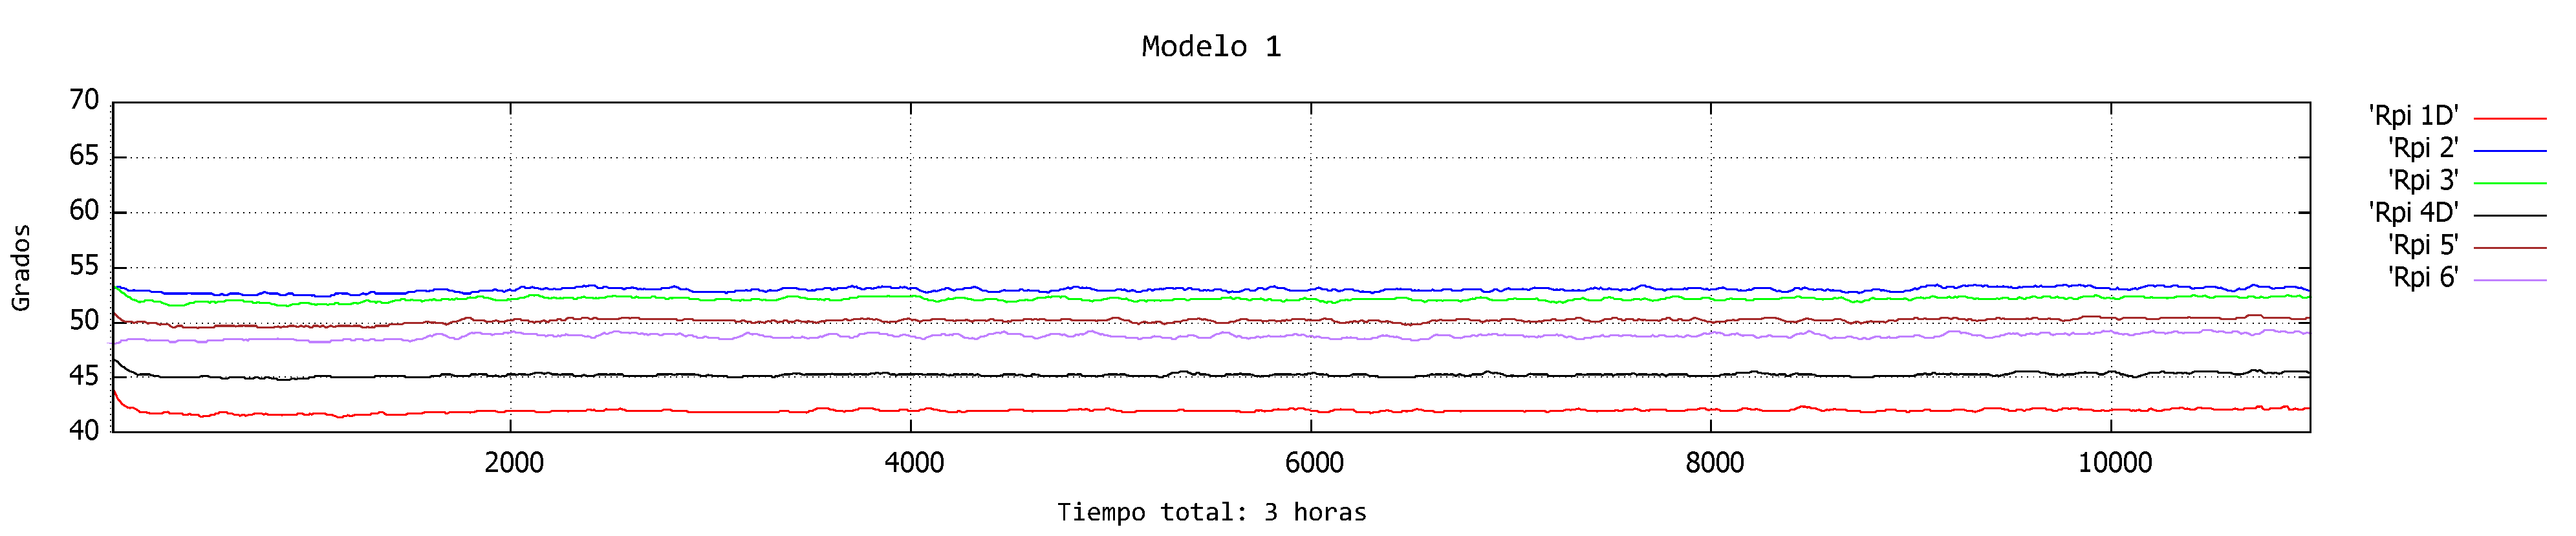
\includegraphics[width=160mm]{Test/pr3_modelo1.pdf}
   	\caption[Prueba 3, Modelo 1]{Modelo 1}
   \label{figure5.9}
\end{figure}


\begin{figure}[H]
	\centering
  	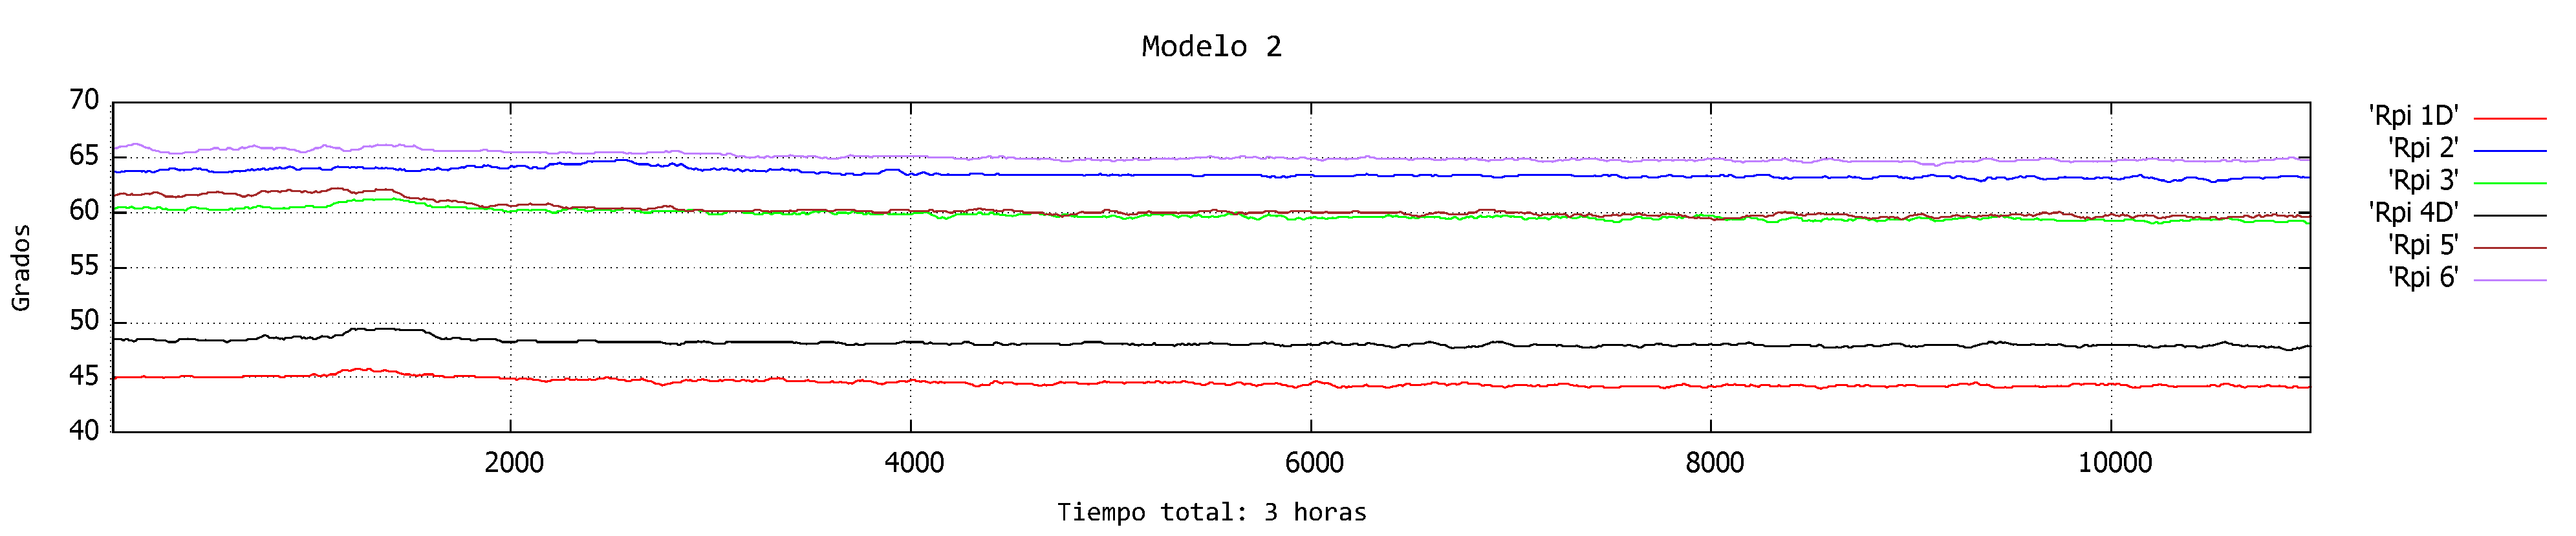
\includegraphics[width=160mm]{Test/pr3_modelo2.pdf}
   	\caption[Prueba 3, Modelo 2]{Modelo 2}
   \label{figure5.10}
\end{figure}

\begin{figure}[H]
	\centering
  	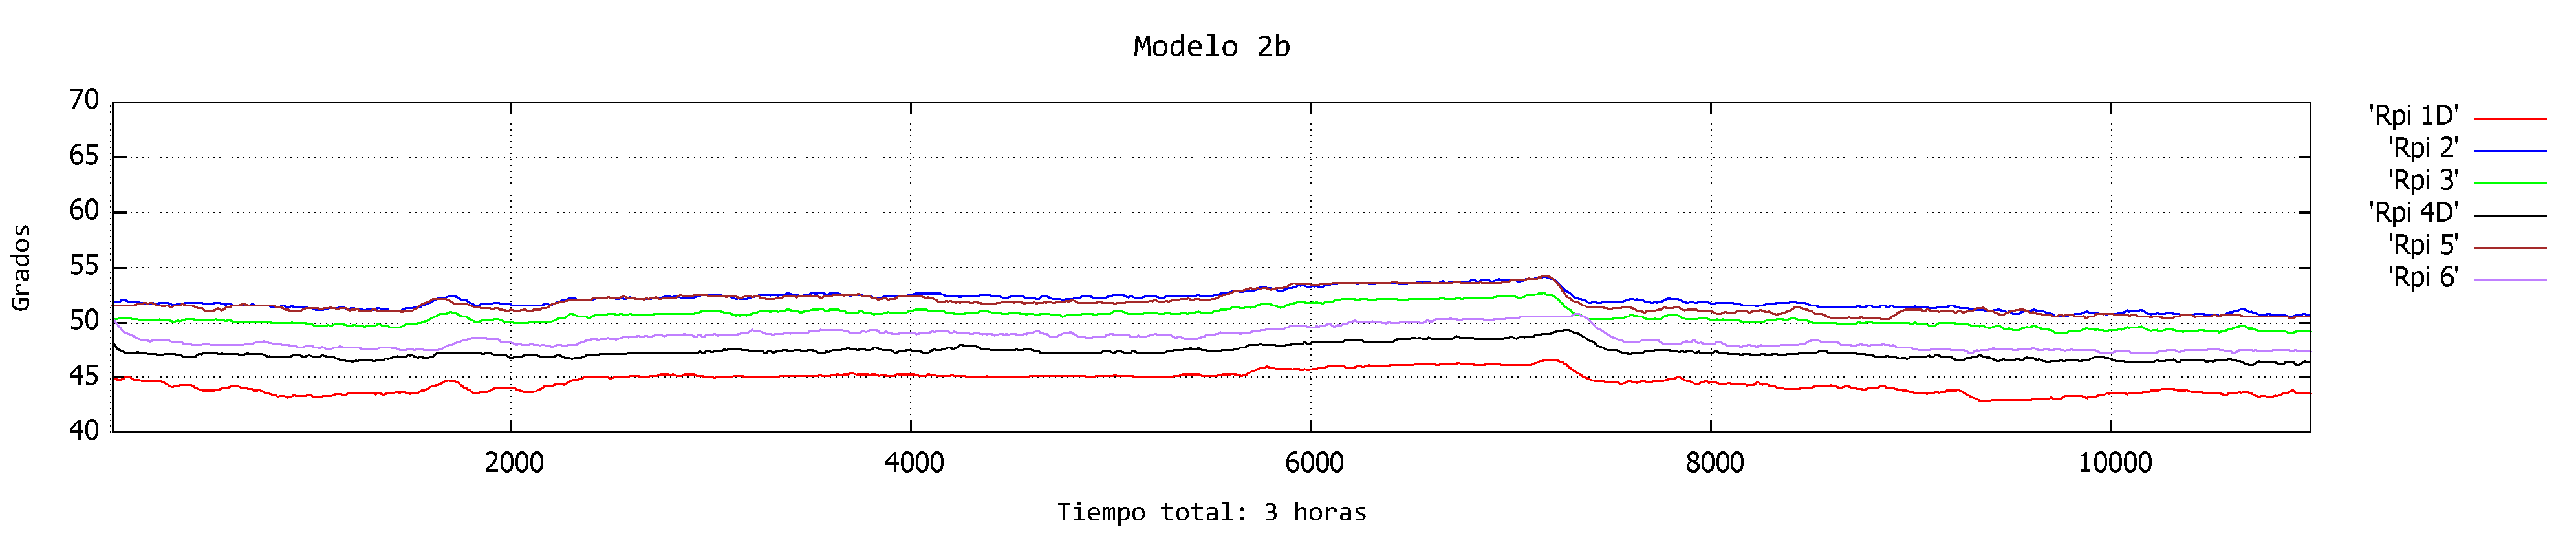
\includegraphics[width=160mm]{Test/pr3_modelo2b.pdf}
   	\caption[Prueba 3, Modelo 2b]{Modelo 2b}
   \label{figure5.11}
\end{figure}

\begin{figure}[H]
	\centering
  	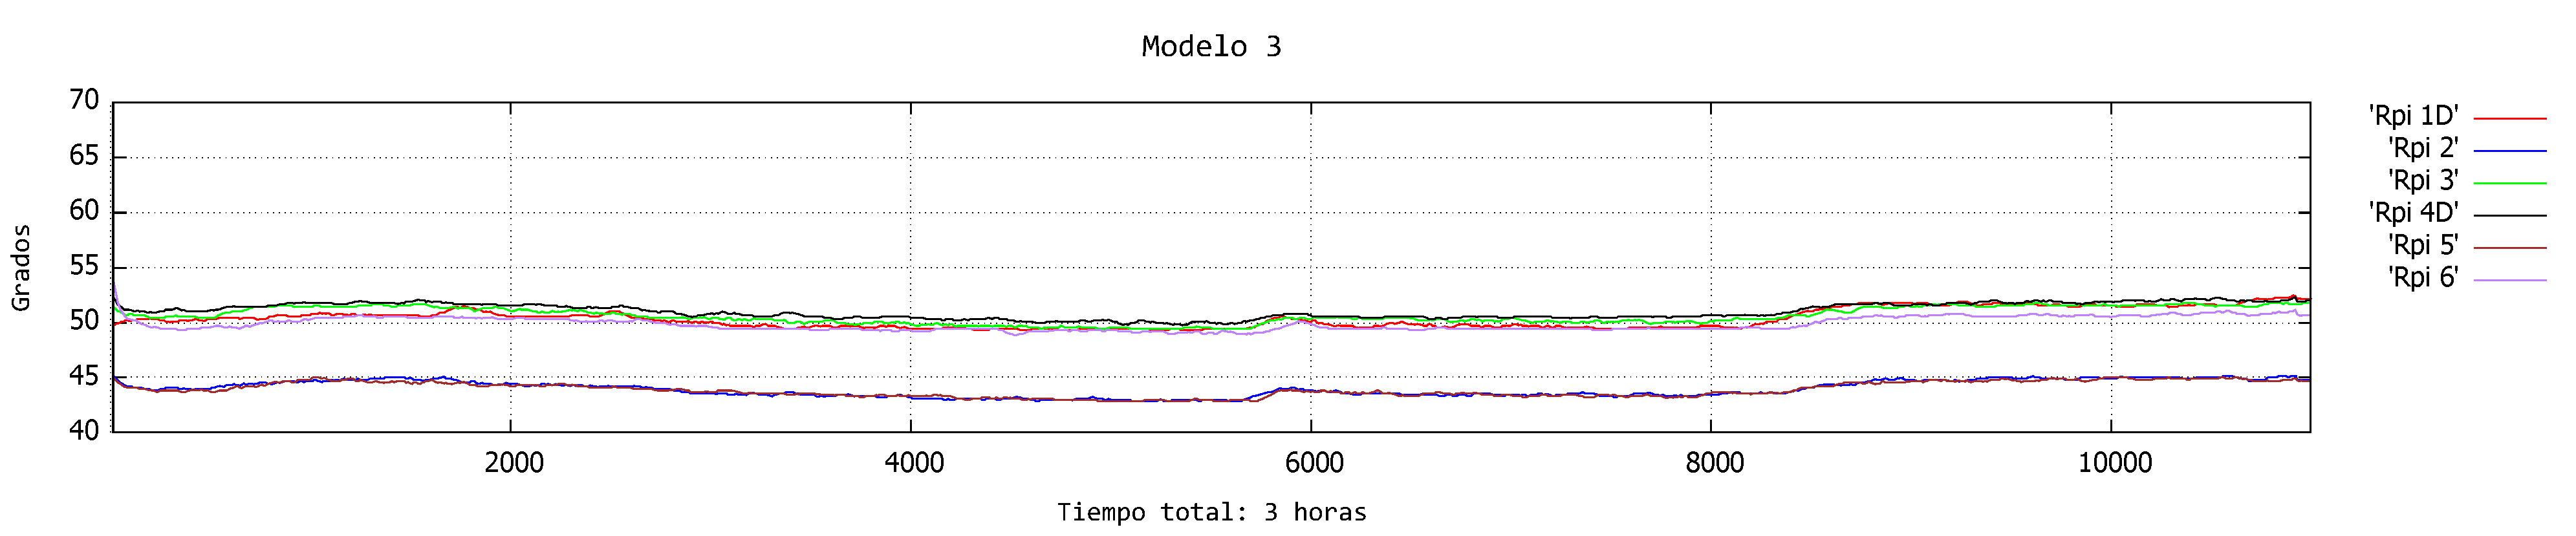
\includegraphics[width=160mm]{Test/pr3_modelo3.pdf}
   	\caption[Prueba 3, Modelo 3]{Modelo 3}
   \label{figure5.12}
\end{figure}

\subsection{Conclusiones}
\paragraph{}
En esta prueba hemos detectado que definitivamente el modelo 2 no cumple con las expectativas necesarias para el correcto funcionamiento del clúster, en él, las diferencias entre nodos con y sin disipador son muy notables y aquellas que no disponen de esta mejora arrojan unas temperaturas muy próximas a los ochenta grados, temperatura crítica de parada, por lo que podemos descartar este modelo para el desarrollo final.

Los otros tres modelos ofrecen unos resultados semejantes a las anteriores pruebas, particularmente el modelo 1 sigue mostrando gran diferencia entre los nodos con disipador. El modelo 2b, aunque ofrece algunas variaciones más notables durante la prueba, sigue manteniendo una relación parecida entre nodos, independientemente de que incluya o no disipadores.

El modelo 3 presenta los mejores resultados, manteniendo temperaturas bajas cercanas a los cincuenta grados y una notable diferencia entrelas Raspberrys que disponen de disipador, las cuales se mantienen en cuarenta y cinco grados. 

\section{Prueba 4}

\label{makereference5.6}
\subsection{Escenario}
\paragraph{}

El objetivo de esta última prueba es comprobar el comportamiento del sistema durante un periodo de tiempo largo. Se realizó sobre el modelo 1 durante venticuatro horas de forma ininterrumpida. El escenario es similar al de la prueba 3, con seis Raspberrys trabajando en paraleleo,  sin embargo, este muestreo se realiza cada sesenta segundos. No podemos certificar la temperatura ambiente para toda la prueba, pero calculamos que osciló entre los quince y dieciocho grados.

\subsection{Resultados}

\begin{figure}[H]
	\centering
  	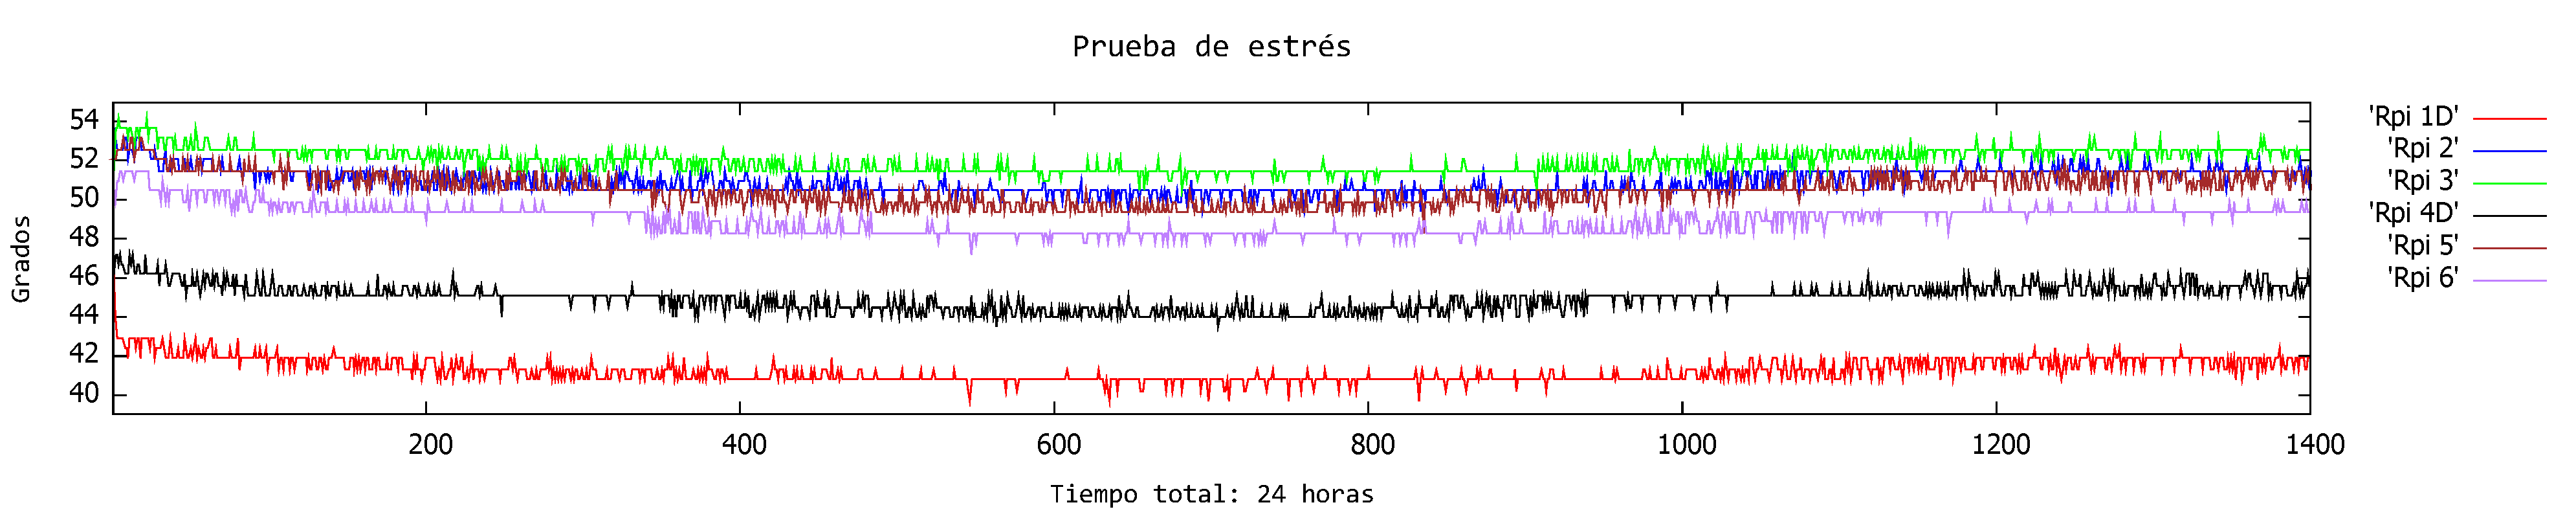
\includegraphics[width=175mm]{Test/pr4_estres.pdf}
   	\caption[Prueba 4, Prueba de estrés]{Resultados}
   \label{figure5.13}
\end{figure}

\subsection{Conclusiones}

Prueba de estrés

\section{Conclusiones generales}
\label{makereference5.7}
\paragraph{}

Durante el desarrollo de los test hemos podido apreciar algunos de los diferentes factores más influyentes sobre el sistema, a continuación, destacamos los que han sido más notorios:

\begin{enumerate}

\item Las \textit{corrientes de aire} tienen una gran afección, merece la pena dedicar parte del trabajo a buscar una eficiencia en la conducción de flujos de aire dentro del contenedor, una buena distribución de la entrada y salida de aire nos permite reducir el número de ventiladores y establecer un punto de partida para la disposición del resto de elementos.

\item Al contar con un gran número de cables, también es necesario combinar el punto anterior con la \textit{accesibilidad general a los dispositivos}, de esta manera, exponiendo las tarjetas SD conseguimos que no sea necesario abrir el contenedor para acceder a cada uno de los nodos.

\item La \textit{temperatura ambiente} es otro de los factores influyentes en el comportamiento general, aunque menos notorio, se pueden apreciar alteraciones en todos los dispositivos sujetos a este efecto. Sería preciso que ésta se mantuviera lo más estable posible.

\item En cuanto a la \textit{robustez}, los resultados ofrecidos por la prueba de estrés, figura \ref{figure5.13}, muestran que el comportamiento ha sido similar al del resto de pruebas, independientemente del número de horas, por lo que podemos concluir que el sistema es fiable y poco propenso a las caídas repentinas por periodos largos de trabajo.

\item En las diferentes pruebas realizadas hemos observado que \textit{no existe una correlación entre tasa de trabajo completado y temperatura}. Aún así, con el fin de prolongar la vida útil de cada nodo, siempre es mejor mantener un rango de temperaturas bajo.

\item El uso de \textit{disipadores} es muy conveniente, son elementos de precio reducido, y con una distribución de aire adecuada aumentan tanto la vida útil del clúster, como el comportamiento de los nodos ante los cambios bruscos de temperatura ambiente. En el peor de los casos, todos los nodos que disponían de esta mejora ofrecieron unos resultados inferiores a los del resto.

\end{enumerate}

\newpage

\thispagestyle{empty}
\mbox{}

\chapter{Cliente Servidor en JAVA}

\label{ch:capitulo6.tex}

\begin{FraseCelebre}
	\begin{Frase}
		'long long long' is too long for GCC
	\end{Frase}
	\begin{Fuente}
	Some GCC programer
	\end{Fuente}
\end{FraseCelebre}

La introducción que creamos necesaria para este capítulo

\section{Creación de un .jar}
\label{makereference6.2}
\paragraph{}

Para poder ejecutar los \textit{.jar} correctamente debemos tener nuestra versión de \textit{Java} en la \textbf{versión 1.8}, esto se configura de la siguiente manera:

\begin{lstlisting}[language=c,frame=single,numbers=none]
	1 sudo update-alternatives --config java
	2 Elegiremos la opción /usr/lib/jvm/oracle-java8-jdk-i386/jre/bin/java
	3 En caso de que no se encuentre:
		3.1	sudo apt-get upgrade
		3.2	sudo apt-get update
		3.3	sudo apt-get install default-jre
	Dentro de eclipse:
	4 Seleccionamos: Proyect - export - runnable JAR file
		4.2	launch configuration elegimos la clase que queremos hacer ejecutable (client.java o server.java)
		4.3 opiones seleccionadas: 
        	4.3.1 extract required libraries into generated jar
		4.4 finish
    
\end{lstlisting}


	
	 



\newpage

\thispagestyle{empty}
\mbox{}

\chapter{Presupuesto}

\label{ch:capitulo7.tex}

\begin{FraseCelebre}
	\begin{Frase}
		No te engañes Jimmy. Si una vaca tuviera la oportunidad, te comería a ti, y a los seres que tú mas quieres.
	\end{Frase}
	\begin{Fuente}
	 Troy McClure
	\end{Fuente}
\end{FraseCelebre}


\begin{enumerate}

\item Pruebas de temperatura con el modelo final
\item Pruebas de rendimiento con el modelo final
\item Código en Java


\end{enumerate}


\vspace{5mm} %5mm vertical space
\vfill

\begin{figure}[H]
	\centering
	
\includegraphics[width=150mm]{pics/theend.png}
\end{figure}

\appendix
\input{referencias.tex}

\end{document}
